\documentclass[a4paper,10pt]{article}
\usepackage[T1]{fontenc}
\usepackage[utf8]{inputenc}
\usepackage[nonumberlist,nopostdot]{glossaries-extra}     % provides glossary commands
\usepackage{graphicx}       % provides commands for including figures
\usepackage{amsmath}

% Glossary needs to be before \begin{document}
\newglossaryentry{ID}
{
  name=ID,
  plural=IDs,
  description={
    An ID is a string of digits, english letters (both lower- and uppercase) and slashes '-'.
  }
}
\newglossaryentry{job status}
{
  name=job status,
  plural=job status,
  description={
    The status of a job can be:
    \begin{itemize}
      \item Queued - the job is waiting for a suitable work machine to become available.
      \item Running - the job is running on some work machine.
      \item Paused - the job has been running, but has been paused to allow for execution of other jobs.
      \item Done - the job has finished running.
      \item Killed - the job was forcefully stopped.
      \item Crashed - the work machine the job was running on shut down unexpectedly.
    \end{itemize}
  }
}
\newglossaryentry{job priority}
{
  name=job priority,
  plural=job priorities,
  description={
    The priority of a job can be one of the following (in ascending order):
    \begin{itemize}
      \item Low
      \item Medium
      \item High
      \item Urgent
    \end{itemize}
  }
}
\newglossaryentry{job}
{
  name=job,
  plural=jobs,
  description={
      A job in the context of JobAdder consists of the following:
      \begin{itemize}
        \item A unique job \gls{ID}.
        \item A program to be executed.
        \item A unix user who owns the job.
        \item \Gls{job priority}.
        \item Number of CPU threads needed for the execution of the program, an integer.
        \item Amount of RAM in megabytes needed for the execution of the program, an integer.
        \item Paths in the network storage needed for the application.
        \item One of:
        \begin{itemize}
          \item A Dockerfile providing instructions to build program environment.
          \item The name of predefined container environment, for ex. a base image from Docker Hub.
        \end{itemize}
     \end{itemize}
  }
}
\newglossaryentry{timestamp}
{
  name=timestamp,
  plural=timestamps,
  description={
    A timestamp is a combination of the date and time of a particular point in time.
    It has the following format: "YYYY-DD-MM HH:MM:SS".
  }
}
\newglossaryentry{administrator}
{
  name=administrator,
  plural=administrators,
  description={
    An administrator is a user who can terminate queued and running jobs from all users.
  }
}
\newglossaryentry{UID}
{
  name=UID,
  plural=UIDs,
  description={
    A UID (user identifier) is a number assigned by Linux to each user on the system.
  }
}
\newglossaryentry{GID}
{
  name=GID,
  plural=GIDs,
  description={
    A GID (group identifier) is a number assigned by Linux to each group on the system.
  }
}
\newglossaryentry{Dockerfile}
{
  name=Dockerfile,
  plural=Dockerfiles,
  description={
     A Dockerfile is a text document that contains all the commands a user could call on the
     command line to assemble an image.
  }
}


%opening
\title{JobAdder: Requirements}
\author{}

\begin{document}

% Macro for table of contents from sections instead of chapters
% Taken from https://tex.stackexchange.com/questions/246354/change-toc-to-section-instead-of-chapter
\makeatletter
\renewcommand\tableofcontents{%
    \if@twocolumn
      \@restonecoltrue\onecolumn
    \else
      \@restonecolfalse
    \fi
    \section*{\contentsname
        \@mkboth{%
           \MakeUppercase\contentsname}{\MakeUppercase\contentsname}}%
    \@starttoc{toc}%
    \if@restonecol\twocolumn\fi
    }
\makeatother

\maketitle
\tableofcontents
\newpage

\section{Introduction}
The JobAdder project enables users to remotely execute resource-intensive tasks on a dedicated cluster of work machines.
Tasks are being distributed to work machines automatically.\newline
The distribution reduces task execution times and peak system loads by better utilizing the available hardware.
In addition, JobAdder provides tools to inspect the state of the whole system and display statistics about user activity.
\section{Purpose}
  \subsection{Product Goal}
    JobAdder aims to facilitate and accelerate the execution of computationally
    expensive jobs in a cluster of work machines.

    Currently, users need to access every single work machine manually in order to
    distribute their jobs over them. Even more problems arise when a group of users
    is involved. In that case, users have to look for the work machine with the
    least amount of work and add their job to it.
   
    JobAdder addresses and solves these problems. With JobAdder, users are able to
    send their jobs to a central server in order to evenly distribute them over
    suitable work machines without having to look for them manually. So if there is
    enough workload (which is usually the case), no machine remains idle unless it
    is forced to.

    Jobadder also aims to make task scheduling more user-friendly. A user does not
    have to keep checking the state of their job, they will be notified once the job
    is done. Nor does a user have to wait for an idle machine in order to queue a
    job, the central server saves them up and runs them once it is possible. There
    is also more insight into the whole system by providing statistics about user
    activity, currently running jobs, past jobs and queued jobs.
   
    Users can set priorities for their jobs so that jobs with high priority will be
    executed before jobs with low priority. Urgent jobs are immediately executed by
    pausing jobs with the lowest priority, so a user is not required to pause or
    cancel low-priority jobs manually. The scheduling algorithm also guarantees that
    every job is eventually run by automatically increasing it's priority over time.

  \subsection{Target Audience}
    The target audience mostly consists of groups of users with access to several
    work machines. This includes, companies, academic institutions and computing
    centers. These users usually need remote machines to run their jobs due to high
    hardware requirements.
   
    JobAdder helps them use their hardware more efficiently by adding an abstraction
    layer between the user and the work machines that are running the user's jobs.
\newpage
\documentclass[a4paper,10pt]{scrreprt}
\usepackage[T1]{fontenc}
\usepackage[utf8]{inputenc}
\usepackage[nonumberlist,nopostdot]{glossaries-extra}     % provides glossary commands
\usepackage{graphicx}       % provides commands for including figures
\usepackage{amsmath}
\usepackage{float}
\usepackage{hyperref}

% Glossary needs to be before \begin{document}
\newglossaryentry{ID}
{
  name=ID,
  plural=IDs,
  description={
    An ID is a string of digits, english letters (both lower- and uppercase) and slashes '-'.
  }
}
\newglossaryentry{job status}
{
  name=job status,
  plural=job status,
  description={
    The status of a job can be:
    \begin{itemize}
      \item Queued - the job is waiting for a suitable work machine to become available.
      \item Running - the job is running on some work machine.
      \item Paused - the job has been running, but has been paused to allow for execution of other jobs.
      \item Done - the job has finished running.
      \item Killed - the job was forcefully stopped.
      \item Crashed - the work machine the job was running on shut down unexpectedly.
    \end{itemize}
  }
}
\newglossaryentry{job priority}
{
  name=job priority,
  plural=job priorities,
  description={
    The priority of a job can be one of the following (in ascending order):
    \begin{itemize}
      \item Low
      \item Medium
      \item High
      \item Urgent
    \end{itemize}
  }
}
\newglossaryentry{job}
{
  name=job,
  plural=jobs,
  description={
      A job in the context of JobAdder consists of the following:
      \begin{itemize}
        \item A unique job \gls{ID}.
        \item A program to be executed.
        \item A unix user who owns the job.
        \item \Gls{job priority}.
        \item Number of CPU threads needed for the execution of the program, an integer.
        \item Amount of RAM in megabytes needed for the execution of the program, an integer.
        \item Paths in the network storage needed for the application.
        \item One of:
        \begin{itemize}
          \item A Dockerfile providing instructions to build program environment.
          \item The name of predefined container environment, for ex. a base image from Docker Hub.
        \end{itemize}
     \end{itemize}
  }
}
\newglossaryentry{timestamp}
{
  name=timestamp,
  plural=timestamps,
  description={
    A timestamp is a combination of the date and time of a particular point in time.
    It has the following format: "YYYY-DD-MM HH:MM:SS".
  }
}
\newglossaryentry{administrator}
{
  name=administrator,
  plural=administrators,
  description={
    An administrator is a user who can terminate queued and running jobs from all users.
  }
}
\newglossaryentry{UID}
{
  name=UID,
  plural=UIDs,
  description={
    A UID (user identifier) is a number assigned by Linux to each user on the system.
  }
}
\newglossaryentry{GID}
{
  name=GID,
  plural=GIDs,
  description={
    A GID (group identifier) is a number assigned by Linux to each group on the system.
  }
}
\newglossaryentry{Dockerfile}
{
  name=Dockerfile,
  plural=Dockerfiles,
  description={
     A Dockerfile is a text document that contains all the commands a user could call on the
     command line to assemble an image.
  }
}


%opening
\title{JobAdder: Requirements}
\author{Johannes Gäßler \and  Ilia Bozhinov \and Nikola Tzotchev \and Malik Bouguila \and Jamil Bagga}

\begin{document}

\maketitle
\tableofcontents
\newpage

\section{Introduction}
The JobAdder project enables users to remotely execute resource-intensive tasks on a dedicated cluster of work machines.
Tasks are being distributed to work machines automatically.\newline
The distribution reduces task execution times and peak system loads by better utilizing the available hardware.
In addition, JobAdder provides tools to inspect the state of the whole system and display statistics about user activity.
\section{Purpose}
  \subsection{Product Goal}
    JobAdder aims to facilitate and accelerate the execution of computationally
    expensive jobs in a cluster of work machines.

    Currently, users need to access every single work machine manually in order to
    distribute their jobs over them. Even more problems arise when a group of users
    is involved. In that case, users have to look for the work machine with the
    least amount of work and add their job to it.
   
    JobAdder addresses and solves these problems. With JobAdder, users are able to
    send their jobs to a central server in order to evenly distribute them over
    suitable work machines without having to look for them manually. So if there is
    enough workload (which is usually the case), no machine remains idle unless it
    is forced to.

    Jobadder also aims to make task scheduling more user-friendly. A user does not
    have to keep checking the state of their job, they will be notified once the job
    is done. Nor does a user have to wait for an idle machine in order to queue a
    job, the central server saves them up and runs them once it is possible. There
    is also more insight into the whole system by providing statistics about user
    activity, currently running jobs, past jobs and queued jobs.
   
    Users can set priorities for their jobs so that jobs with high priority will be
    executed before jobs with low priority. Urgent jobs are immediately executed by
    pausing jobs with the lowest priority, so a user is not required to pause or
    cancel low-priority jobs manually. The scheduling algorithm also guarantees that
    every job is eventually run by automatically increasing it's priority over time.

  \subsection{Target Audience}
    The target audience mostly consists of groups of users with access to several
    work machines. This includes, companies, academic institutions and computing
    centers. These users usually need remote machines to run their jobs due to high
    hardware requirements.
   
    JobAdder helps them use their hardware more efficiently by adding an abstraction
    layer between the user and the work machines that are running the user's jobs.
\documentclass[a4paper,10pt]{scrreprt}
\usepackage[T1]{fontenc}
\usepackage[utf8]{inputenc}
\usepackage[nonumberlist,nopostdot]{glossaries-extra}     % provides glossary commands
\usepackage{graphicx}       % provides commands for including figures
\usepackage{amsmath}
\usepackage{float}
\usepackage{hyperref}

% Glossary needs to be before \begin{document}
\newglossaryentry{ID}
{
  name=ID,
  plural=IDs,
  description={
    An ID is a string of digits, english letters (both lower- and uppercase) and slashes '-'.
  }
}
\newglossaryentry{job status}
{
  name=job status,
  plural=job status,
  description={
    The status of a job can be:
    \begin{itemize}
      \item Queued - the job is waiting for a suitable work machine to become available.
      \item Running - the job is running on some work machine.
      \item Paused - the job has been running, but has been paused to allow for execution of other jobs.
      \item Done - the job has finished running.
      \item Killed - the job was forcefully stopped.
      \item Crashed - the work machine the job was running on shut down unexpectedly.
    \end{itemize}
  }
}
\newglossaryentry{job priority}
{
  name=job priority,
  plural=job priorities,
  description={
    The priority of a job can be one of the following (in ascending order):
    \begin{itemize}
      \item Low
      \item Medium
      \item High
      \item Urgent
    \end{itemize}
  }
}
\newglossaryentry{job}
{
  name=job,
  plural=jobs,
  description={
      A job in the context of JobAdder consists of the following:
      \begin{itemize}
        \item A unique job \gls{ID}.
        \item A program to be executed.
        \item A unix user who owns the job.
        \item \Gls{job priority}.
        \item Number of CPU threads needed for the execution of the program, an integer.
        \item Amount of RAM in megabytes needed for the execution of the program, an integer.
        \item Paths in the network storage needed for the application.
        \item One of:
        \begin{itemize}
          \item A Dockerfile providing instructions to build program environment.
          \item The name of predefined container environment, for ex. a base image from Docker Hub.
        \end{itemize}
     \end{itemize}
  }
}
\newglossaryentry{timestamp}
{
  name=timestamp,
  plural=timestamps,
  description={
    A timestamp is a combination of the date and time of a particular point in time.
    It has the following format: "YYYY-DD-MM HH:MM:SS".
  }
}
\newglossaryentry{administrator}
{
  name=administrator,
  plural=administrators,
  description={
    An administrator is a user who can terminate queued and running jobs from all users.
  }
}
\newglossaryentry{UID}
{
  name=UID,
  plural=UIDs,
  description={
    A UID (user identifier) is a number assigned by Linux to each user on the system.
  }
}
\newglossaryentry{GID}
{
  name=GID,
  plural=GIDs,
  description={
    A GID (group identifier) is a number assigned by Linux to each group on the system.
  }
}
\newglossaryentry{Dockerfile}
{
  name=Dockerfile,
  plural=Dockerfiles,
  description={
     A Dockerfile is a text document that contains all the commands a user could call on the
     command line to assemble an image.
  }
}


%opening
\title{JobAdder: Requirements}
\author{Johannes Gäßler \and  Ilia Bozhinov \and Nikola Tzotchev \and Malik Bouguila \and Jamil Bagga}

\begin{document}

\maketitle
\tableofcontents
\newpage

\section{Introduction}
The JobAdder project enables users to remotely execute resource-intensive tasks on a dedicated cluster of work machines.
Tasks are being distributed to work machines automatically.\newline
The distribution reduces task execution times and peak system loads by better utilizing the available hardware.
In addition, JobAdder provides tools to inspect the state of the whole system and display statistics about user activity.
\section{Purpose}
  \subsection{Product Goal}
    JobAdder aims to facilitate and accelerate the execution of computationally
    expensive jobs in a cluster of work machines.

    Currently, users need to access every single work machine manually in order to
    distribute their jobs over them. Even more problems arise when a group of users
    is involved. In that case, users have to look for the work machine with the
    least amount of work and add their job to it.
   
    JobAdder addresses and solves these problems. With JobAdder, users are able to
    send their jobs to a central server in order to evenly distribute them over
    suitable work machines without having to look for them manually. So if there is
    enough workload (which is usually the case), no machine remains idle unless it
    is forced to.

    Jobadder also aims to make task scheduling more user-friendly. A user does not
    have to keep checking the state of their job, they will be notified once the job
    is done. Nor does a user have to wait for an idle machine in order to queue a
    job, the central server saves them up and runs them once it is possible. There
    is also more insight into the whole system by providing statistics about user
    activity, currently running jobs, past jobs and queued jobs.
   
    Users can set priorities for their jobs so that jobs with high priority will be
    executed before jobs with low priority. Urgent jobs are immediately executed by
    pausing jobs with the lowest priority, so a user is not required to pause or
    cancel low-priority jobs manually. The scheduling algorithm also guarantees that
    every job is eventually run by automatically increasing it's priority over time.

  \subsection{Target Audience}
    The target audience mostly consists of groups of users with access to several
    work machines. This includes, companies, academic institutions and computing
    centers. These users usually need remote machines to run their jobs due to high
    hardware requirements.
   
    JobAdder helps them use their hardware more efficiently by adding an abstraction
    layer between the user and the work machines that are running the user's jobs.
\documentclass[a4paper,10pt]{scrreprt}
\usepackage[T1]{fontenc}
\usepackage[utf8]{inputenc}
\usepackage[nonumberlist,nopostdot]{glossaries-extra}     % provides glossary commands
\usepackage{graphicx}       % provides commands for including figures
\usepackage{amsmath}
\usepackage{float}
\usepackage{hyperref}

% Glossary needs to be before \begin{document}
\input{customer/glossary}

%opening
\title{JobAdder: Requirements}
\author{Johannes Gäßler \and  Ilia Bozhinov \and Nikola Tzotchev \and Malik Bouguila \and Jamil Bagga}

\begin{document}

\maketitle
\tableofcontents
\newpage

\input{customer/introduction}
\input{customer/goals}
\input{customer/main}
\input{customer/product-environment}
\input{customer/scheduling-algorithm}
\input{customer/cli}
\input{system/main}

\newpage
\input{system/systemmodel/use-case-diagram}
\input{system/systemmodel/system-model.tex}

\printunsrtglossaries
\end{document}

\chapter{Product Environment}
  \section{User Client}
    \subsection{Hardware Requirements}
      \begin{itemize}
      \item A connection to the central server.
      \item 2 MB of storage space and an additional 100 MB per image.
      \end{itemize}
    \subsection{Software Requirements}
      \begin{itemize}
      \item Python 3.
    \end{itemize}

  \section{Central Server}
    \subsection{Hardware Requirements}
    \begin{itemize}
      \item 500 MB of storage space.
      \item 2 GB of RAM.
      \item One physical CPU core.
    \end{itemize}
    \subsection{Software Requirements}
    \begin{itemize}
      \item Linux Ubuntu 18.04 or newer, or CentOS 7.5 or newer.
      \item MySQL Database Server version 8.0 or newer.
      \item Linux kernel version 3.10 or higher.
      \item CS Docker engine 1.13, EE Deamon 17.03 and higher.
      \item Python 3.
    \end{itemize}

  \section{Working Machine Client}
    \subsection{Hardware Requirements}
      In addition to the hardware required to run a job, our worker client would need the following resources:
    \begin{itemize}
      \item A connection to a LAN.
      \item 4 GB of RAM.
      \item 3 GB of available disk space.
      \item Static IP Address.
    \end{itemize}
    \subsection{Software Requirements}
    \begin{itemize}
      \item Linux kernel version 3.10 or higher.
      \item CS Docker engine 1.13, EE Deamon 17.03 and higher.
      \item Python 3.
    \end{itemize}


\subsection{Scheduling Algorithm}
This section describes how the central server distributes jobs to work machines: the \textit{scheduling algorithm}.
Put briefly, the scheduling algorithm takes a list of jobs and decides which ones to run on the available work machines.
The scheduling algorithm has the following goals:
\begin{itemize}
\item Keep work machines busy: there should be no idle work machines if there are pending jobs.
\item Consider job priorities: jobs with high priorities should be worked on first.
\item Consider time of job submission: jobs that were submitted first should be worked on first (if priorities are equal).
\end{itemize}
The scheduling algorithm operates under the following conditions:
\begin{itemize}
\item Jobs arrive at unforeseen times.
\item Time required to complete jobs is unknown.
\item Jobs cannot be transferred from one work machine to another.
\item Jobs cannot be canceled and restarted.
\item Job preemption is limited: if a job is paused it has to be kept in memory.
Note that memory includes swap files.
\item Some jobs cannot be paused due to software licensing restrictions.
\end{itemize}
The scheduling algorithm takes the following parameters as input:
\begin{itemize}
\item List of pending jobs.
\item List of running/paused jobs per work machine.
\item Amount of work machine specific resources: CPU threads, memory, etc.
These resources can typically be freed by pausing jobs.
\item Amount of work machine unspecific resources: software licenses.
Whether these resources can be freed by pausing jobs depends on the software.
\item Size of work machine swap files.
This resource is used exclusively for holding paused jobs.
It has no influence on running jobs.
\end{itemize}
The scheduling algorithm reevaluates which jobs to run every time a job finishes running or when a new job request arrives.
The scheduling algorithm assigns jobs to work machines as follows:
\begin{enumerate}
\item If there are pending urgent jobs:
Assign oldest urgent jobs to work machines until urgent jobs or resources run out.
Non-urgent running jobs will be paused if possible and necessary to run more urgent jobs.
\item If there are paused high-priority jobs:
Assign oldest paused high-priority jobs to work machines until paused high-priority jobs or resources run out.
Running jobs with equal or lower priority will be paused if possible and necessary to run more old paused high-priority jobs.
\item Repeat 2. for paused medium-priority jobs.
\item Repeat 2. for paused low-priority jobs.
\item If there are pending high-priority jobs:
Assign oldest paused high-priority jobs to work machines until paused high-priority jobs or resources run out.
Running jobs with equal or lower priority will be paused if possible and necessary to run the oldest available high-priority job.
\item Repeat 5. for pending medium-priority jobs.
\item Repeat 5. for pending low-priority jobs.
\end{enumerate}
\newcommand{\jacommand}[3]{
\textsc{\LARGE{\textbf{#1}}}
\begin{itemize}
\item \textbf{Options:} #2
\item \textbf{Effect:} #3
\end{itemize}
}
\newcommand{\jaoptionheader}{\textsc{\textbf{Option descriptions:}}\newline\newline}
\newcommand{\jaoption}[3]{
\textbf{#1}
\begin{itemize}
\item \textbf{Short form:} #2
\item \textbf{Effect:} #3
\end{itemize}
}
\subsection{Command Line Interface}
All components of JobAdder are accessible through a command line interface (CLI).
The command line interface on a machine with JobAdder installed has the following structure:
\begin{equation}
\text{<component name> <command> <options> <targets>},
\end{equation}
where the \textit{component name} can be any one of the following:
\begin{itemize}
\item \textbf{jobadder} to access the \textit{user client}.
\item \textbf{jobcenter} to access the \textit{server}.
\item \textbf{jobworker} to access the \textit{worker client}.
\end{itemize}
Commands, options, and valid targets are and options are specified in the following sections.

Options can be added in the following ways:
\begin{itemize}
\item By supplying their names like "-{}-option\_x -{}-option\_y=2 -{}-option\_z".
\item By supplying their abbreviations like "-x -y 2 -z".
\item By supplying their abbreviations like "-xz -y 2".
\end{itemize}

The available \textit{commands} are generally specific to the used component.
Likewise, the available \textit{options} and \textit{targets} are generally specific to the commands of a used component.
However, some commands and options are shared between components or commands.

The JobAdder CLI only uses lower-case letters.
JobAdder CLI options override the values of configuration files.
If no command is given, the general help text for the given component is printed out.
\subsubsection{Shared Options}
\jaoption{config}{c}{Overrides the global configuration file with the given configuration file.}
\jaoption{detach}{d}{Detaches the execution of the given command from the command line.}
\jaoption{help}{h}{
Prints out a list of the available commands. 
When used in conjunction with a command:
prints out more detailed information on the given command and a list of the available options.}
\jaoption{verbose}{v}{
Determines the amount of information printed out.
If set to 2, detailed information is printed out.
If set to 1, only high-level information is printed out (default).
If set to 0, no information is printed out.}
\subsubsection{User Client}
\jacommand{add}
{gpu, mount, name, priority, server, ram, threads}
{Sends one or more job requests to the server.
If targets are Docker containers the job consists of simply running the container.
If targets are configuration files with a specified terminal command the job consists of running the specified terminal command.
Otherwise targets are interpreted as terminal commands}
\jaoptionheader
\jaoption{gpu}{g}{
If set to true, informs the server that the job requires a gpu.
If set to a string that can be interpreted as VRAM amount, informs the server that a GPU with this amount of VRAM is required for the job.
If set to a specific GPU model, informs the server that the job must be run on a machine with that GPU built in.
}
\jaoption{mount}{m}
{Directories that need to be mounted onto the Docker container that the job is running in.}
\jaoption{name}{n}
{Human-readable name of the job.
Defaults to user's name + job index}
\jaoption{priority}{p}
{Sets the priority of the job: urgent, high, medium, or low.
Defaults to medium.}
\jaoption{server}{s}
{Server to send the job request to.
Defaults to localhost.}
\jaoption{ram}{r}
{If set to a string that can be interpreted as RAM amount, informs the server that this amount of RAM is required for the job.}
\jaoption{threads}{t}
{If set to an integer, informs the server that this number of threads is required for the job.}
\jacommand{query}{user}
{Prints out information on running/queued/past jobs (specified by target).
In addition to the one below, options from add command can be used as constraints.}
\jaoptionheader
\jaoption{after}{a}{Only return jobs added after the given point in time.}
\jaoption{before}{b}{Only return jobs added before the given point in time.}
\jaoption{user}{u}{Filter query by user that added the job.}
\jacommand{stop}{None}{Stops the job with the specified name.}
\subsubsection{Server}
\jacommand{start}{None}{Starts an instance of the JobAdder server.}
\jacommand{stop}{None}{Stops instances of the JobAdder server.}
\subsubsection{Worker Client}
\jacommand{start}{server}{Starts an instance of the JobAdder worker client.}
\jaoptionheader
\jaoption{server}{s}
{Server to receive jobs from.
Defaults to localhost.}
\jacommand{stop}{None}{Stops instances of the JobAdder worker client.}

\documentclass[a4paper,10pt]{scrreprt}
\usepackage[T1]{fontenc}
\usepackage[utf8]{inputenc}
\usepackage[nonumberlist,nopostdot]{glossaries-extra}     % provides glossary commands
\usepackage{graphicx}       % provides commands for including figures
\usepackage{amsmath}
\usepackage{float}
\usepackage{hyperref}

% Glossary needs to be before \begin{document}
\input{customer/glossary}

%opening
\title{JobAdder: Requirements}
\author{Johannes Gäßler \and  Ilia Bozhinov \and Nikola Tzotchev \and Malik Bouguila \and Jamil Bagga}

\begin{document}

\maketitle
\tableofcontents
\newpage

\input{customer/introduction}
\input{customer/goals}
\input{customer/main}
\input{customer/product-environment}
\input{customer/scheduling-algorithm}
\input{customer/cli}
\input{system/main}

\newpage
\input{system/systemmodel/use-case-diagram}
\input{system/systemmodel/system-model.tex}

\printunsrtglossaries
\end{document}


\newpage
\subsection{Use Case Diagram}
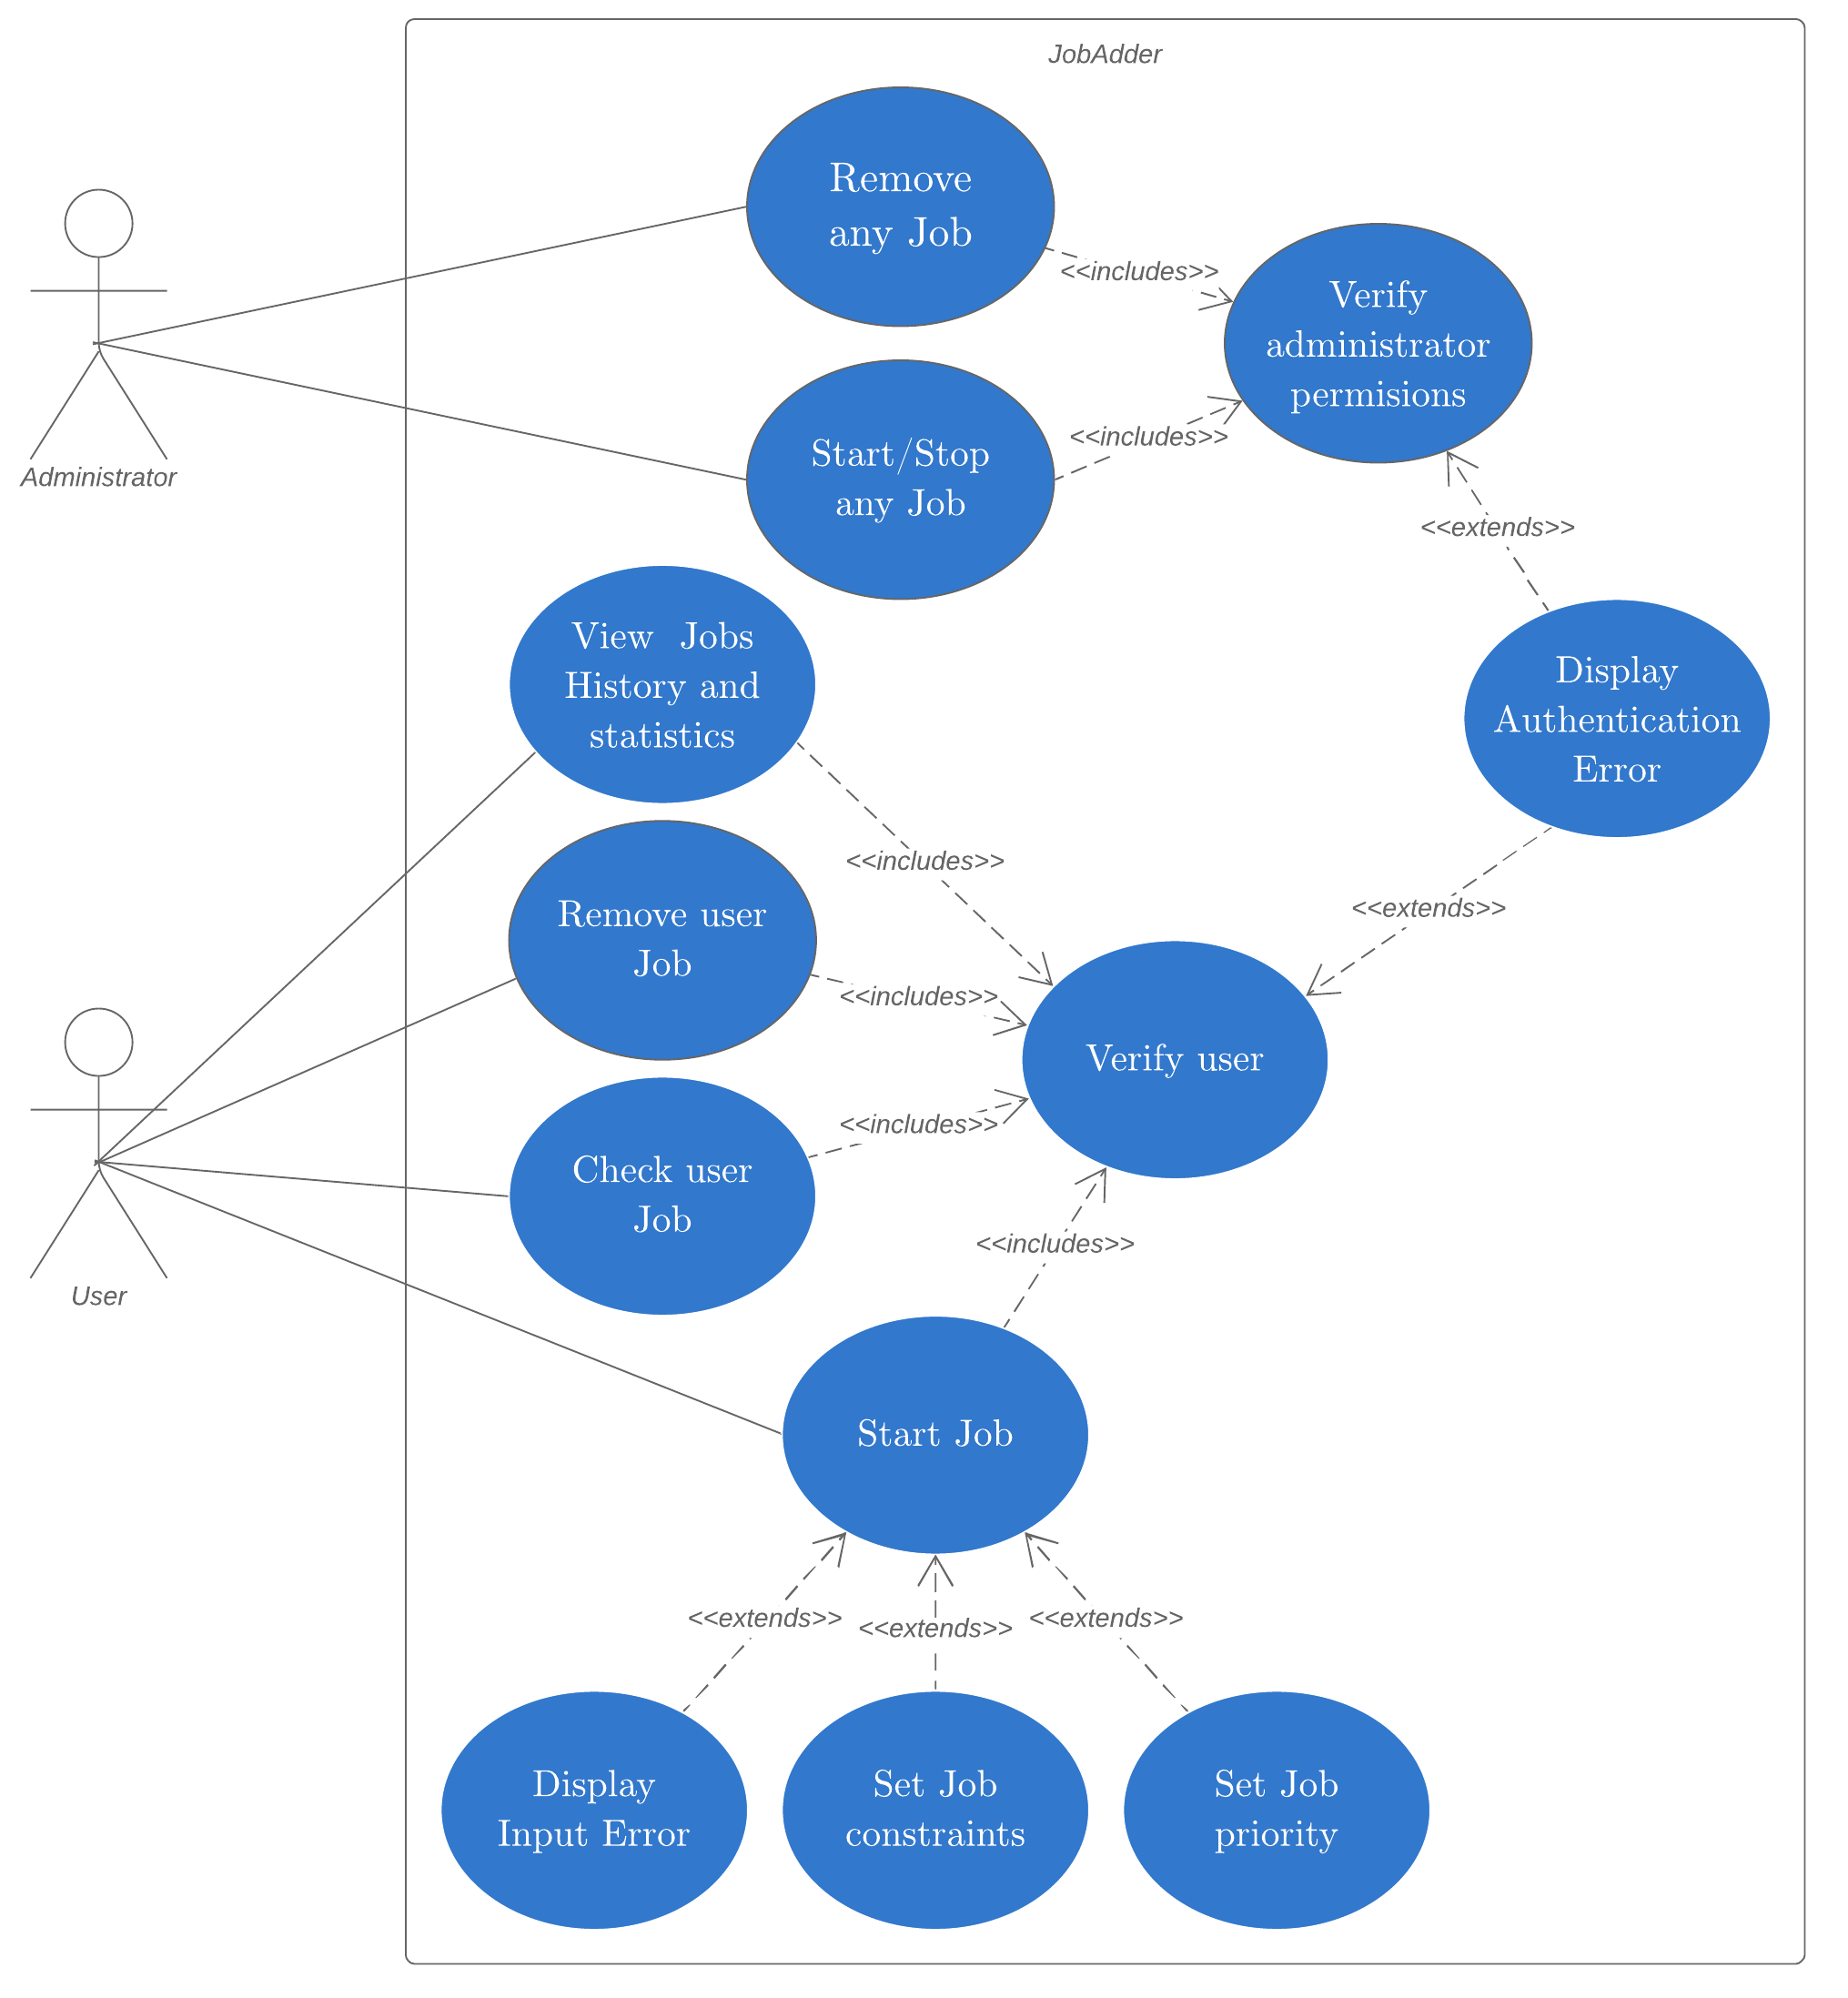
\includegraphics[width=\linewidth]{./system/systemmodel/images/usecasediagram.png}

\subsection{System Model}
\begin{figure}
  \subsubsection{Schedule new Job}
  \centering
  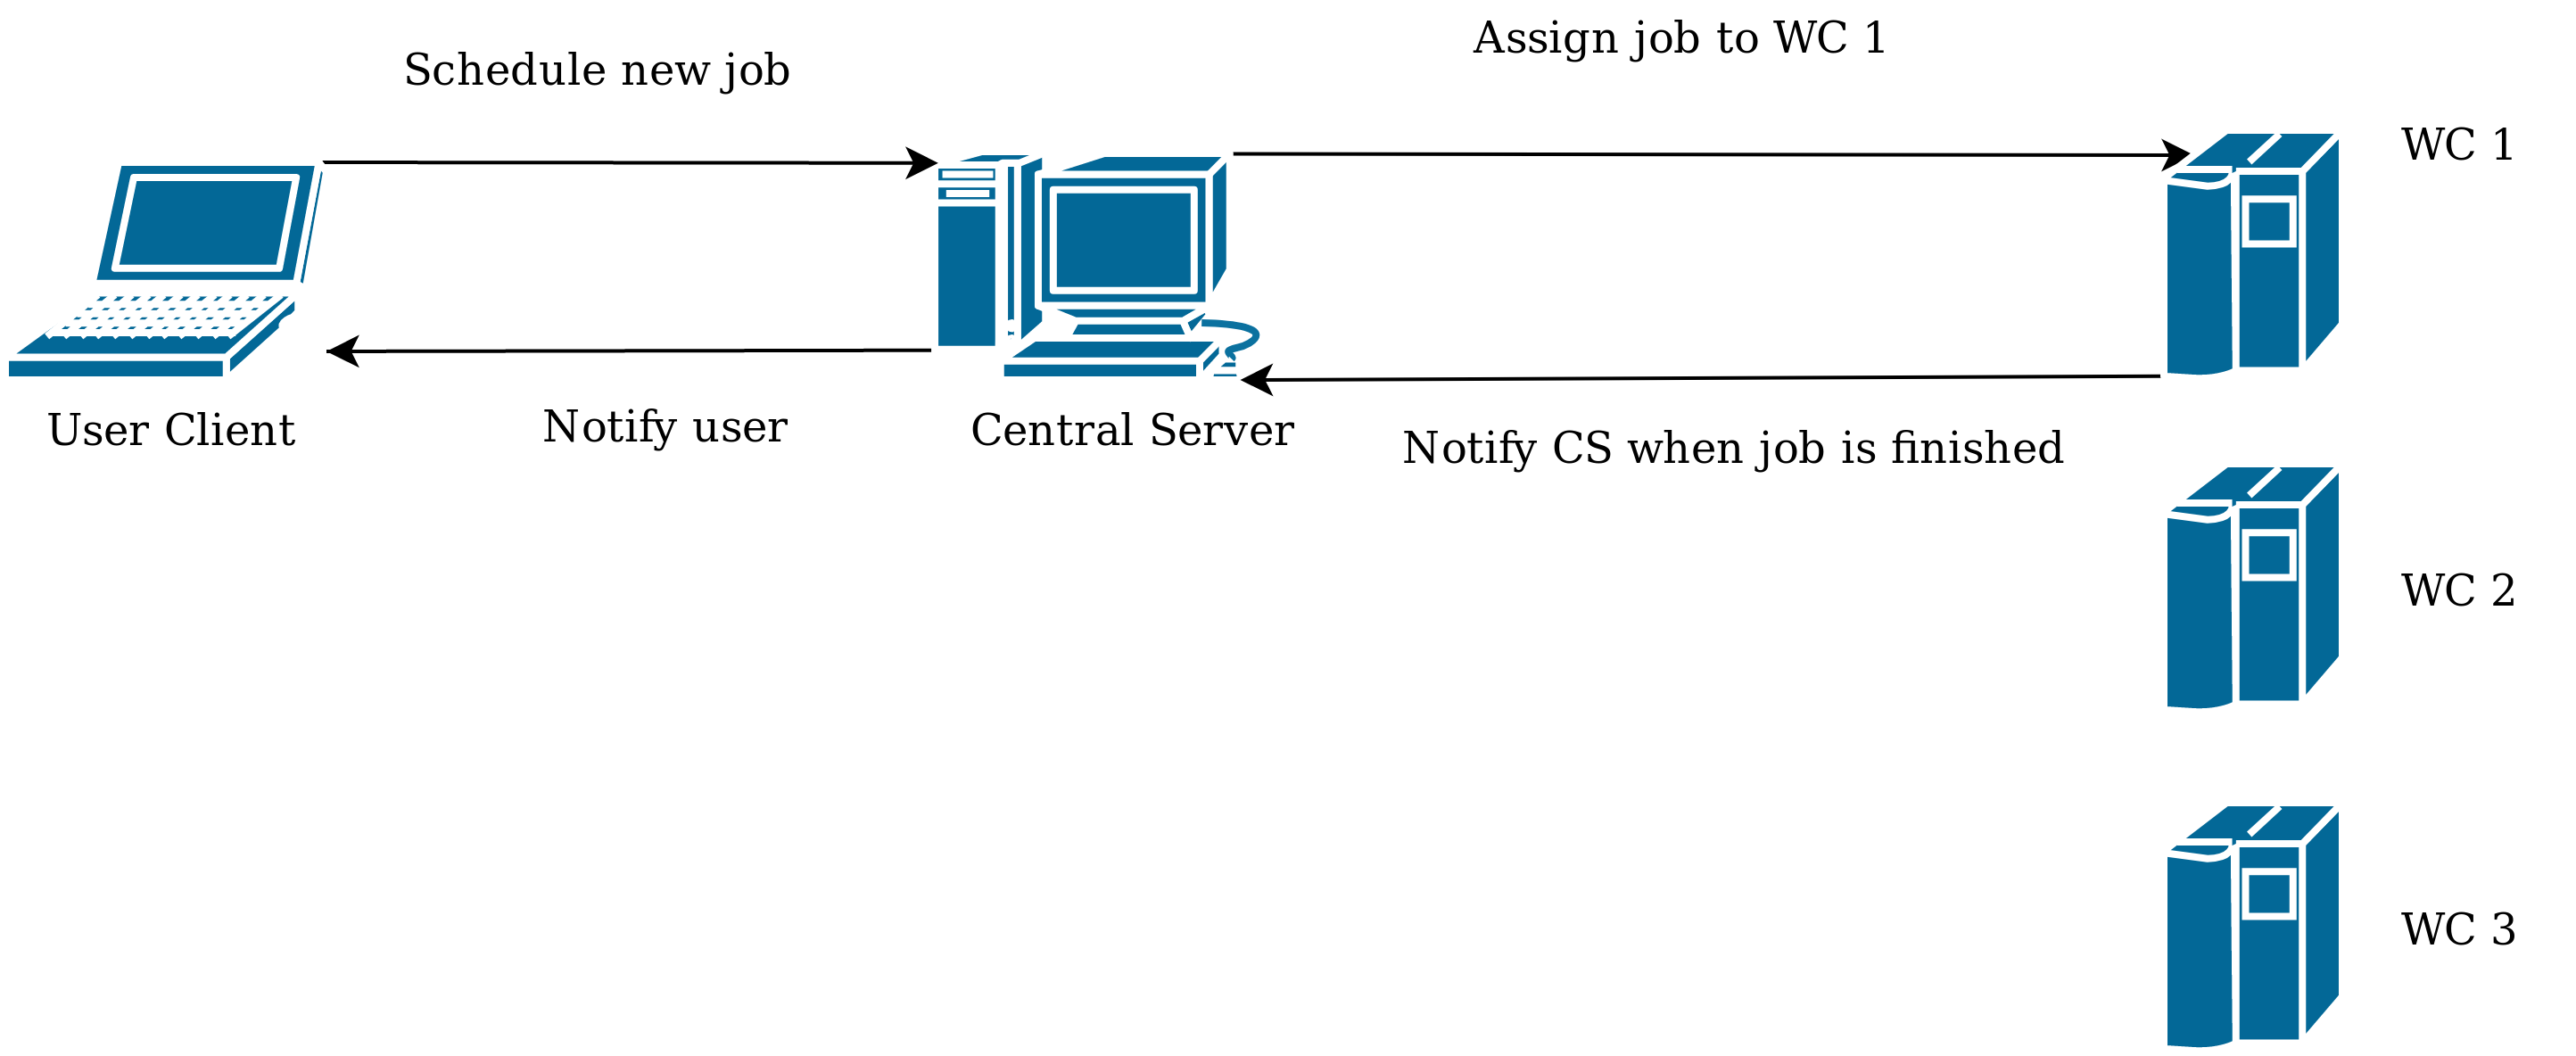
\includegraphics[width=\linewidth]{./system/systemmodel/images/schedulejob.png}
  \label{new-job}
  \caption{This diagram depicts how a user schedules a job, which the CS distributes to WC 1.
  In that case CS knows that there are enough resurces on WC 1 to execute users job.
  At the end the CS notifies the user that the job has finished.}
\end{figure}

\begin{figure}
  \subsubsection{Access a job}
  \centering
  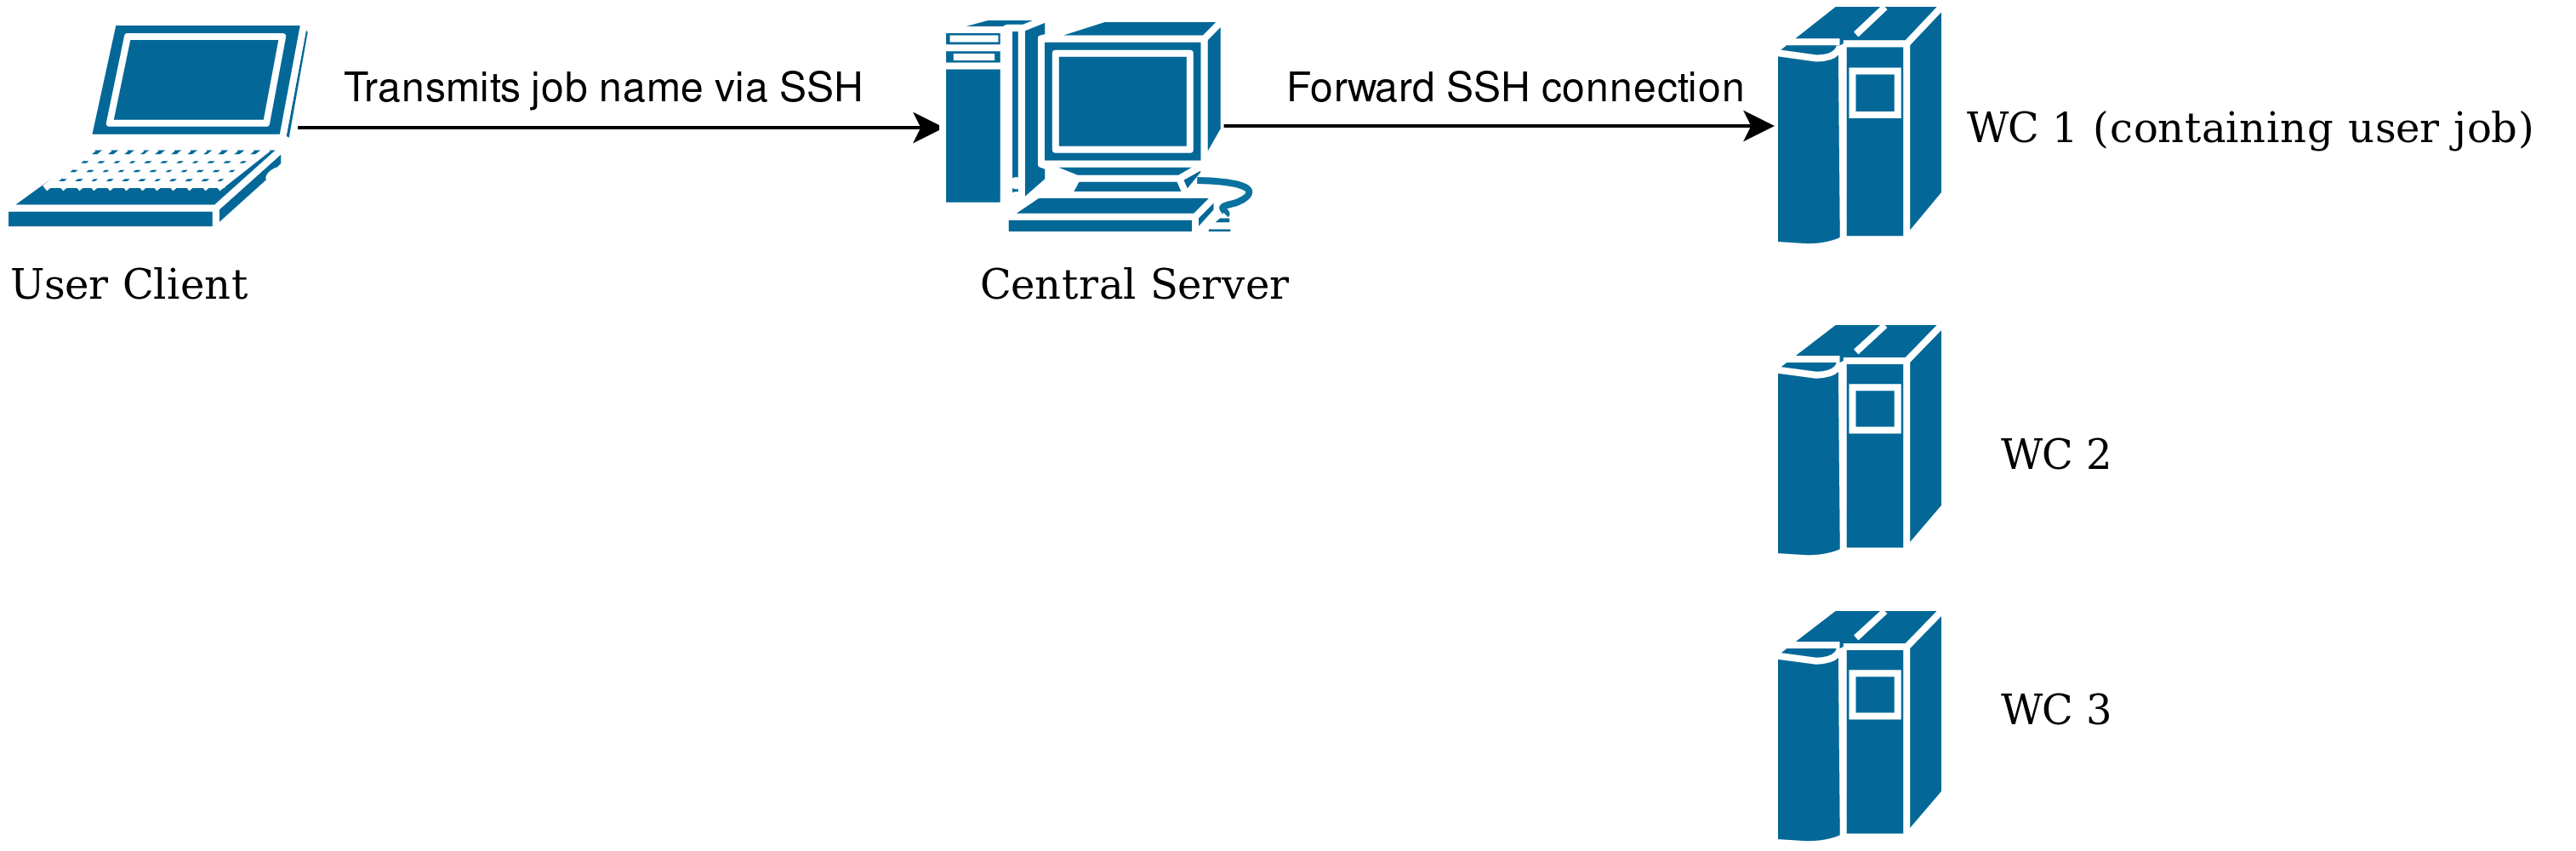
\includegraphics[width=\linewidth]{./system/systemmodel/images/accessjob.png}
  \label{access-job}
  \caption{This diagram depicts how a user accesses his job.
  The user has a job on one of the work machines that he wants to connect to.
  The user does not establish a direct connection with the WC.
  The user establishes an SSH connection to the server.
  This connection authenticates the user.
  It is also used to transmit the name of the job that the user wants to connect to.
  The server looks up which work machine the user's job is located on and forwards the SSH connection to that work machine.
  Finally, the SSH connection to the work machine is forwarded to the container with the user's job.}
\end{figure}

\begin{figure}
  \subsubsection{Get statistics}
  \centering
  
\includegraphics[width=0.5\linewidth]{./system/systemmodel/images/statistics.png}
  \label{statistics}
  \caption{This diagram depicts how a user accesses the statistics saved on the server.}
\end{figure}


\printunsrtglossaries
\end{document}

\chapter{Product Environment}
  \section{User Client}
    \subsection{Hardware Requirements}
      \begin{itemize}
      \item A connection to the central server.
      \item 2 MB of storage space and an additional 100 MB per image.
      \end{itemize}
    \subsection{Software Requirements}
      \begin{itemize}
      \item Python 3.
    \end{itemize}

  \section{Central Server}
    \subsection{Hardware Requirements}
    \begin{itemize}
      \item 500 MB of storage space.
      \item 2 GB of RAM.
      \item One physical CPU core.
    \end{itemize}
    \subsection{Software Requirements}
    \begin{itemize}
      \item Linux Ubuntu 18.04 or newer, or CentOS 7.5 or newer.
      \item MySQL Database Server version 8.0 or newer.
      \item Linux kernel version 3.10 or higher.
      \item CS Docker engine 1.13, EE Deamon 17.03 and higher.
      \item Python 3.
    \end{itemize}

  \section{Working Machine Client}
    \subsection{Hardware Requirements}
      In addition to the hardware required to run a job, our worker client would need the following resources:
    \begin{itemize}
      \item A connection to a LAN.
      \item 4 GB of RAM.
      \item 3 GB of available disk space.
      \item Static IP Address.
    \end{itemize}
    \subsection{Software Requirements}
    \begin{itemize}
      \item Linux kernel version 3.10 or higher.
      \item CS Docker engine 1.13, EE Deamon 17.03 and higher.
      \item Python 3.
    \end{itemize}


\subsection{Scheduling Algorithm}
This section describes how the central server distributes jobs to work machines: the \textit{scheduling algorithm}.
Put briefly, the scheduling algorithm takes a list of jobs and decides which ones to run on the available work machines.
The scheduling algorithm has the following goals:
\begin{itemize}
\item Keep work machines busy: there should be no idle work machines if there are pending jobs.
\item Consider job priorities: jobs with high priorities should be worked on first.
\item Consider time of job submission: jobs that were submitted first should be worked on first (if priorities are equal).
\end{itemize}
The scheduling algorithm operates under the following conditions:
\begin{itemize}
\item Jobs arrive at unforeseen times.
\item Time required to complete jobs is unknown.
\item Jobs cannot be transferred from one work machine to another.
\item Jobs cannot be canceled and restarted.
\item Job preemption is limited: if a job is paused it has to be kept in memory.
Note that memory includes swap files.
\item Some jobs cannot be paused due to software licensing restrictions.
\end{itemize}
The scheduling algorithm takes the following parameters as input:
\begin{itemize}
\item List of pending jobs.
\item List of running/paused jobs per work machine.
\item Amount of work machine specific resources: CPU threads, memory, etc.
These resources can typically be freed by pausing jobs.
\item Amount of work machine unspecific resources: software licenses.
Whether these resources can be freed by pausing jobs depends on the software.
\item Size of work machine swap files.
This resource is used exclusively for holding paused jobs.
It has no influence on running jobs.
\end{itemize}
The scheduling algorithm reevaluates which jobs to run every time a job finishes running or when a new job request arrives.
The scheduling algorithm assigns jobs to work machines as follows:
\begin{enumerate}
\item If there are pending urgent jobs:
Assign oldest urgent jobs to work machines until urgent jobs or resources run out.
Non-urgent running jobs will be paused if possible and necessary to run more urgent jobs.
\item If there are paused high-priority jobs:
Assign oldest paused high-priority jobs to work machines until paused high-priority jobs or resources run out.
Running jobs with equal or lower priority will be paused if possible and necessary to run more old paused high-priority jobs.
\item Repeat 2. for paused medium-priority jobs.
\item Repeat 2. for paused low-priority jobs.
\item If there are pending high-priority jobs:
Assign oldest paused high-priority jobs to work machines until paused high-priority jobs or resources run out.
Running jobs with equal or lower priority will be paused if possible and necessary to run the oldest available high-priority job.
\item Repeat 5. for pending medium-priority jobs.
\item Repeat 5. for pending low-priority jobs.
\end{enumerate}
\newcommand{\jacommand}[3]{
\textsc{\LARGE{\textbf{#1}}}
\begin{itemize}
\item \textbf{Options:} #2
\item \textbf{Effect:} #3
\end{itemize}
}
\newcommand{\jaoptionheader}{\textsc{\textbf{Option descriptions:}}\newline\newline}
\newcommand{\jaoption}[3]{
\textbf{#1}
\begin{itemize}
\item \textbf{Short form:} #2
\item \textbf{Effect:} #3
\end{itemize}
}
\subsection{Command Line Interface}
All components of JobAdder are accessible through a command line interface (CLI).
The command line interface on a machine with JobAdder installed has the following structure:
\begin{equation}
\text{<component name> <command> <options> <targets>},
\end{equation}
where the \textit{component name} can be any one of the following:
\begin{itemize}
\item \textbf{jobadder} to access the \textit{user client}.
\item \textbf{jobcenter} to access the \textit{server}.
\item \textbf{jobworker} to access the \textit{worker client}.
\end{itemize}
Commands, options, and valid targets are and options are specified in the following sections.

Options can be added in the following ways:
\begin{itemize}
\item By supplying their names like "-{}-option\_x -{}-option\_y=2 -{}-option\_z".
\item By supplying their abbreviations like "-x -y 2 -z".
\item By supplying their abbreviations like "-xz -y 2".
\end{itemize}

The available \textit{commands} are generally specific to the used component.
Likewise, the available \textit{options} and \textit{targets} are generally specific to the commands of a used component.
However, some commands and options are shared between components or commands.

The JobAdder CLI only uses lower-case letters.
JobAdder CLI options override the values of configuration files.
If no command is given, the general help text for the given component is printed out.
\subsubsection{Shared Options}
\jaoption{config}{c}{Overrides the global configuration file with the given configuration file.}
\jaoption{detach}{d}{Detaches the execution of the given command from the command line.}
\jaoption{help}{h}{
Prints out a list of the available commands. 
When used in conjunction with a command:
prints out more detailed information on the given command and a list of the available options.}
\jaoption{verbose}{v}{
Determines the amount of information printed out.
If set to 2, detailed information is printed out.
If set to 1, only high-level information is printed out (default).
If set to 0, no information is printed out.}
\subsubsection{User Client}
\jacommand{add}
{gpu, mount, name, priority, server, ram, threads}
{Sends one or more job requests to the server.
If targets are Docker containers the job consists of simply running the container.
If targets are configuration files with a specified terminal command the job consists of running the specified terminal command.
Otherwise targets are interpreted as terminal commands}
\jaoptionheader
\jaoption{gpu}{g}{
If set to true, informs the server that the job requires a gpu.
If set to a string that can be interpreted as VRAM amount, informs the server that a GPU with this amount of VRAM is required for the job.
If set to a specific GPU model, informs the server that the job must be run on a machine with that GPU built in.
}
\jaoption{mount}{m}
{Directories that need to be mounted onto the Docker container that the job is running in.}
\jaoption{name}{n}
{Human-readable name of the job.
Defaults to user's name + job index}
\jaoption{priority}{p}
{Sets the priority of the job: urgent, high, medium, or low.
Defaults to medium.}
\jaoption{server}{s}
{Server to send the job request to.
Defaults to localhost.}
\jaoption{ram}{r}
{If set to a string that can be interpreted as RAM amount, informs the server that this amount of RAM is required for the job.}
\jaoption{threads}{t}
{If set to an integer, informs the server that this number of threads is required for the job.}
\jacommand{query}{user}
{Prints out information on running/queued/past jobs (specified by target).
In addition to the one below, options from add command can be used as constraints.}
\jaoptionheader
\jaoption{after}{a}{Only return jobs added after the given point in time.}
\jaoption{before}{b}{Only return jobs added before the given point in time.}
\jaoption{user}{u}{Filter query by user that added the job.}
\jacommand{stop}{None}{Stops the job with the specified name.}
\subsubsection{Server}
\jacommand{start}{None}{Starts an instance of the JobAdder server.}
\jacommand{stop}{None}{Stops instances of the JobAdder server.}
\subsubsection{Worker Client}
\jacommand{start}{server}{Starts an instance of the JobAdder worker client.}
\jaoptionheader
\jaoption{server}{s}
{Server to receive jobs from.
Defaults to localhost.}
\jacommand{stop}{None}{Stops instances of the JobAdder worker client.}

\documentclass[a4paper,10pt]{scrreprt}
\usepackage[T1]{fontenc}
\usepackage[utf8]{inputenc}
\usepackage[nonumberlist,nopostdot]{glossaries-extra}     % provides glossary commands
\usepackage{graphicx}       % provides commands for including figures
\usepackage{amsmath}
\usepackage{float}
\usepackage{hyperref}

% Glossary needs to be before \begin{document}
\newglossaryentry{ID}
{
  name=ID,
  plural=IDs,
  description={
    An ID is a string of digits, english letters (both lower- and uppercase) and slashes '-'.
  }
}
\newglossaryentry{job status}
{
  name=job status,
  plural=job status,
  description={
    The status of a job can be:
    \begin{itemize}
      \item Queued - the job is waiting for a suitable work machine to become available.
      \item Running - the job is running on some work machine.
      \item Paused - the job has been running, but has been paused to allow for execution of other jobs.
      \item Done - the job has finished running.
      \item Killed - the job was forcefully stopped.
      \item Crashed - the work machine the job was running on shut down unexpectedly.
    \end{itemize}
  }
}
\newglossaryentry{job priority}
{
  name=job priority,
  plural=job priorities,
  description={
    The priority of a job can be one of the following (in ascending order):
    \begin{itemize}
      \item Low
      \item Medium
      \item High
      \item Urgent
    \end{itemize}
  }
}
\newglossaryentry{job}
{
  name=job,
  plural=jobs,
  description={
      A job in the context of JobAdder consists of the following:
      \begin{itemize}
        \item A unique job \gls{ID}.
        \item A program to be executed.
        \item A unix user who owns the job.
        \item \Gls{job priority}.
        \item Number of CPU threads needed for the execution of the program, an integer.
        \item Amount of RAM in megabytes needed for the execution of the program, an integer.
        \item Paths in the network storage needed for the application.
        \item One of:
        \begin{itemize}
          \item A Dockerfile providing instructions to build program environment.
          \item The name of predefined container environment, for ex. a base image from Docker Hub.
        \end{itemize}
     \end{itemize}
  }
}
\newglossaryentry{timestamp}
{
  name=timestamp,
  plural=timestamps,
  description={
    A timestamp is a combination of the date and time of a particular point in time.
    It has the following format: "YYYY-DD-MM HH:MM:SS".
  }
}
\newglossaryentry{administrator}
{
  name=administrator,
  plural=administrators,
  description={
    An administrator is a user who can terminate queued and running jobs from all users.
  }
}
\newglossaryentry{UID}
{
  name=UID,
  plural=UIDs,
  description={
    A UID (user identifier) is a number assigned by Linux to each user on the system.
  }
}
\newglossaryentry{GID}
{
  name=GID,
  plural=GIDs,
  description={
    A GID (group identifier) is a number assigned by Linux to each group on the system.
  }
}
\newglossaryentry{Dockerfile}
{
  name=Dockerfile,
  plural=Dockerfiles,
  description={
     A Dockerfile is a text document that contains all the commands a user could call on the
     command line to assemble an image.
  }
}


%opening
\title{JobAdder: Requirements}
\author{Johannes Gäßler \and  Ilia Bozhinov \and Nikola Tzotchev \and Malik Bouguila \and Jamil Bagga}

\begin{document}

\maketitle
\tableofcontents
\newpage

\section{Introduction}
The JobAdder project enables users to remotely execute resource-intensive tasks on a dedicated cluster of work machines.
Tasks are being distributed to work machines automatically.\newline
The distribution reduces task execution times and peak system loads by better utilizing the available hardware.
In addition, JobAdder provides tools to inspect the state of the whole system and display statistics about user activity.
\section{Purpose}
  \subsection{Product Goal}
    JobAdder aims to facilitate and accelerate the execution of computationally
    expensive jobs in a cluster of work machines.

    Currently, users need to access every single work machine manually in order to
    distribute their jobs over them. Even more problems arise when a group of users
    is involved. In that case, users have to look for the work machine with the
    least amount of work and add their job to it.
   
    JobAdder addresses and solves these problems. With JobAdder, users are able to
    send their jobs to a central server in order to evenly distribute them over
    suitable work machines without having to look for them manually. So if there is
    enough workload (which is usually the case), no machine remains idle unless it
    is forced to.

    Jobadder also aims to make task scheduling more user-friendly. A user does not
    have to keep checking the state of their job, they will be notified once the job
    is done. Nor does a user have to wait for an idle machine in order to queue a
    job, the central server saves them up and runs them once it is possible. There
    is also more insight into the whole system by providing statistics about user
    activity, currently running jobs, past jobs and queued jobs.
   
    Users can set priorities for their jobs so that jobs with high priority will be
    executed before jobs with low priority. Urgent jobs are immediately executed by
    pausing jobs with the lowest priority, so a user is not required to pause or
    cancel low-priority jobs manually. The scheduling algorithm also guarantees that
    every job is eventually run by automatically increasing it's priority over time.

  \subsection{Target Audience}
    The target audience mostly consists of groups of users with access to several
    work machines. This includes, companies, academic institutions and computing
    centers. These users usually need remote machines to run their jobs due to high
    hardware requirements.
   
    JobAdder helps them use their hardware more efficiently by adding an abstraction
    layer between the user and the work machines that are running the user's jobs.
\documentclass[a4paper,10pt]{scrreprt}
\usepackage[T1]{fontenc}
\usepackage[utf8]{inputenc}
\usepackage[nonumberlist,nopostdot]{glossaries-extra}     % provides glossary commands
\usepackage{graphicx}       % provides commands for including figures
\usepackage{amsmath}
\usepackage{float}
\usepackage{hyperref}

% Glossary needs to be before \begin{document}
\input{customer/glossary}

%opening
\title{JobAdder: Requirements}
\author{Johannes Gäßler \and  Ilia Bozhinov \and Nikola Tzotchev \and Malik Bouguila \and Jamil Bagga}

\begin{document}

\maketitle
\tableofcontents
\newpage

\input{customer/introduction}
\input{customer/goals}
\input{customer/main}
\input{customer/product-environment}
\input{customer/scheduling-algorithm}
\input{customer/cli}
\input{system/main}

\newpage
\input{system/systemmodel/use-case-diagram}
\input{system/systemmodel/system-model.tex}

\printunsrtglossaries
\end{document}

\chapter{Product Environment}
  \section{User Client}
    \subsection{Hardware Requirements}
      \begin{itemize}
      \item A connection to the central server.
      \item 2 MB of storage space and an additional 100 MB per image.
      \end{itemize}
    \subsection{Software Requirements}
      \begin{itemize}
      \item Python 3.
    \end{itemize}

  \section{Central Server}
    \subsection{Hardware Requirements}
    \begin{itemize}
      \item 500 MB of storage space.
      \item 2 GB of RAM.
      \item One physical CPU core.
    \end{itemize}
    \subsection{Software Requirements}
    \begin{itemize}
      \item Linux Ubuntu 18.04 or newer, or CentOS 7.5 or newer.
      \item MySQL Database Server version 8.0 or newer.
      \item Linux kernel version 3.10 or higher.
      \item CS Docker engine 1.13, EE Deamon 17.03 and higher.
      \item Python 3.
    \end{itemize}

  \section{Working Machine Client}
    \subsection{Hardware Requirements}
      In addition to the hardware required to run a job, our worker client would need the following resources:
    \begin{itemize}
      \item A connection to a LAN.
      \item 4 GB of RAM.
      \item 3 GB of available disk space.
      \item Static IP Address.
    \end{itemize}
    \subsection{Software Requirements}
    \begin{itemize}
      \item Linux kernel version 3.10 or higher.
      \item CS Docker engine 1.13, EE Deamon 17.03 and higher.
      \item Python 3.
    \end{itemize}


\subsection{Scheduling Algorithm}
This section describes how the central server distributes jobs to work machines: the \textit{scheduling algorithm}.
Put briefly, the scheduling algorithm takes a list of jobs and decides which ones to run on the available work machines.
The scheduling algorithm has the following goals:
\begin{itemize}
\item Keep work machines busy: there should be no idle work machines if there are pending jobs.
\item Consider job priorities: jobs with high priorities should be worked on first.
\item Consider time of job submission: jobs that were submitted first should be worked on first (if priorities are equal).
\end{itemize}
The scheduling algorithm operates under the following conditions:
\begin{itemize}
\item Jobs arrive at unforeseen times.
\item Time required to complete jobs is unknown.
\item Jobs cannot be transferred from one work machine to another.
\item Jobs cannot be canceled and restarted.
\item Job preemption is limited: if a job is paused it has to be kept in memory.
Note that memory includes swap files.
\item Some jobs cannot be paused due to software licensing restrictions.
\end{itemize}
The scheduling algorithm takes the following parameters as input:
\begin{itemize}
\item List of pending jobs.
\item List of running/paused jobs per work machine.
\item Amount of work machine specific resources: CPU threads, memory, etc.
These resources can typically be freed by pausing jobs.
\item Amount of work machine unspecific resources: software licenses.
Whether these resources can be freed by pausing jobs depends on the software.
\item Size of work machine swap files.
This resource is used exclusively for holding paused jobs.
It has no influence on running jobs.
\end{itemize}
The scheduling algorithm reevaluates which jobs to run every time a job finishes running or when a new job request arrives.
The scheduling algorithm assigns jobs to work machines as follows:
\begin{enumerate}
\item If there are pending urgent jobs:
Assign oldest urgent jobs to work machines until urgent jobs or resources run out.
Non-urgent running jobs will be paused if possible and necessary to run more urgent jobs.
\item If there are paused high-priority jobs:
Assign oldest paused high-priority jobs to work machines until paused high-priority jobs or resources run out.
Running jobs with equal or lower priority will be paused if possible and necessary to run more old paused high-priority jobs.
\item Repeat 2. for paused medium-priority jobs.
\item Repeat 2. for paused low-priority jobs.
\item If there are pending high-priority jobs:
Assign oldest paused high-priority jobs to work machines until paused high-priority jobs or resources run out.
Running jobs with equal or lower priority will be paused if possible and necessary to run the oldest available high-priority job.
\item Repeat 5. for pending medium-priority jobs.
\item Repeat 5. for pending low-priority jobs.
\end{enumerate}
\newcommand{\jacommand}[3]{
\textsc{\LARGE{\textbf{#1}}}
\begin{itemize}
\item \textbf{Options:} #2
\item \textbf{Effect:} #3
\end{itemize}
}
\newcommand{\jaoptionheader}{\textsc{\textbf{Option descriptions:}}\newline\newline}
\newcommand{\jaoption}[3]{
\textbf{#1}
\begin{itemize}
\item \textbf{Short form:} #2
\item \textbf{Effect:} #3
\end{itemize}
}
\subsection{Command Line Interface}
All components of JobAdder are accessible through a command line interface (CLI).
The command line interface on a machine with JobAdder installed has the following structure:
\begin{equation}
\text{<component name> <command> <options> <targets>},
\end{equation}
where the \textit{component name} can be any one of the following:
\begin{itemize}
\item \textbf{jobadder} to access the \textit{user client}.
\item \textbf{jobcenter} to access the \textit{server}.
\item \textbf{jobworker} to access the \textit{worker client}.
\end{itemize}
Commands, options, and valid targets are and options are specified in the following sections.

Options can be added in the following ways:
\begin{itemize}
\item By supplying their names like "-{}-option\_x -{}-option\_y=2 -{}-option\_z".
\item By supplying their abbreviations like "-x -y 2 -z".
\item By supplying their abbreviations like "-xz -y 2".
\end{itemize}

The available \textit{commands} are generally specific to the used component.
Likewise, the available \textit{options} and \textit{targets} are generally specific to the commands of a used component.
However, some commands and options are shared between components or commands.

The JobAdder CLI only uses lower-case letters.
JobAdder CLI options override the values of configuration files.
If no command is given, the general help text for the given component is printed out.
\subsubsection{Shared Options}
\jaoption{config}{c}{Overrides the global configuration file with the given configuration file.}
\jaoption{detach}{d}{Detaches the execution of the given command from the command line.}
\jaoption{help}{h}{
Prints out a list of the available commands. 
When used in conjunction with a command:
prints out more detailed information on the given command and a list of the available options.}
\jaoption{verbose}{v}{
Determines the amount of information printed out.
If set to 2, detailed information is printed out.
If set to 1, only high-level information is printed out (default).
If set to 0, no information is printed out.}
\subsubsection{User Client}
\jacommand{add}
{gpu, mount, name, priority, server, ram, threads}
{Sends one or more job requests to the server.
If targets are Docker containers the job consists of simply running the container.
If targets are configuration files with a specified terminal command the job consists of running the specified terminal command.
Otherwise targets are interpreted as terminal commands}
\jaoptionheader
\jaoption{gpu}{g}{
If set to true, informs the server that the job requires a gpu.
If set to a string that can be interpreted as VRAM amount, informs the server that a GPU with this amount of VRAM is required for the job.
If set to a specific GPU model, informs the server that the job must be run on a machine with that GPU built in.
}
\jaoption{mount}{m}
{Directories that need to be mounted onto the Docker container that the job is running in.}
\jaoption{name}{n}
{Human-readable name of the job.
Defaults to user's name + job index}
\jaoption{priority}{p}
{Sets the priority of the job: urgent, high, medium, or low.
Defaults to medium.}
\jaoption{server}{s}
{Server to send the job request to.
Defaults to localhost.}
\jaoption{ram}{r}
{If set to a string that can be interpreted as RAM amount, informs the server that this amount of RAM is required for the job.}
\jaoption{threads}{t}
{If set to an integer, informs the server that this number of threads is required for the job.}
\jacommand{query}{user}
{Prints out information on running/queued/past jobs (specified by target).
In addition to the one below, options from add command can be used as constraints.}
\jaoptionheader
\jaoption{after}{a}{Only return jobs added after the given point in time.}
\jaoption{before}{b}{Only return jobs added before the given point in time.}
\jaoption{user}{u}{Filter query by user that added the job.}
\jacommand{stop}{None}{Stops the job with the specified name.}
\subsubsection{Server}
\jacommand{start}{None}{Starts an instance of the JobAdder server.}
\jacommand{stop}{None}{Stops instances of the JobAdder server.}
\subsubsection{Worker Client}
\jacommand{start}{server}{Starts an instance of the JobAdder worker client.}
\jaoptionheader
\jaoption{server}{s}
{Server to receive jobs from.
Defaults to localhost.}
\jacommand{stop}{None}{Stops instances of the JobAdder worker client.}

\documentclass[a4paper,10pt]{scrreprt}
\usepackage[T1]{fontenc}
\usepackage[utf8]{inputenc}
\usepackage[nonumberlist,nopostdot]{glossaries-extra}     % provides glossary commands
\usepackage{graphicx}       % provides commands for including figures
\usepackage{amsmath}
\usepackage{float}
\usepackage{hyperref}

% Glossary needs to be before \begin{document}
\input{customer/glossary}

%opening
\title{JobAdder: Requirements}
\author{Johannes Gäßler \and  Ilia Bozhinov \and Nikola Tzotchev \and Malik Bouguila \and Jamil Bagga}

\begin{document}

\maketitle
\tableofcontents
\newpage

\input{customer/introduction}
\input{customer/goals}
\input{customer/main}
\input{customer/product-environment}
\input{customer/scheduling-algorithm}
\input{customer/cli}
\input{system/main}

\newpage
\input{system/systemmodel/use-case-diagram}
\input{system/systemmodel/system-model.tex}

\printunsrtglossaries
\end{document}


\newpage
\subsection{Use Case Diagram}
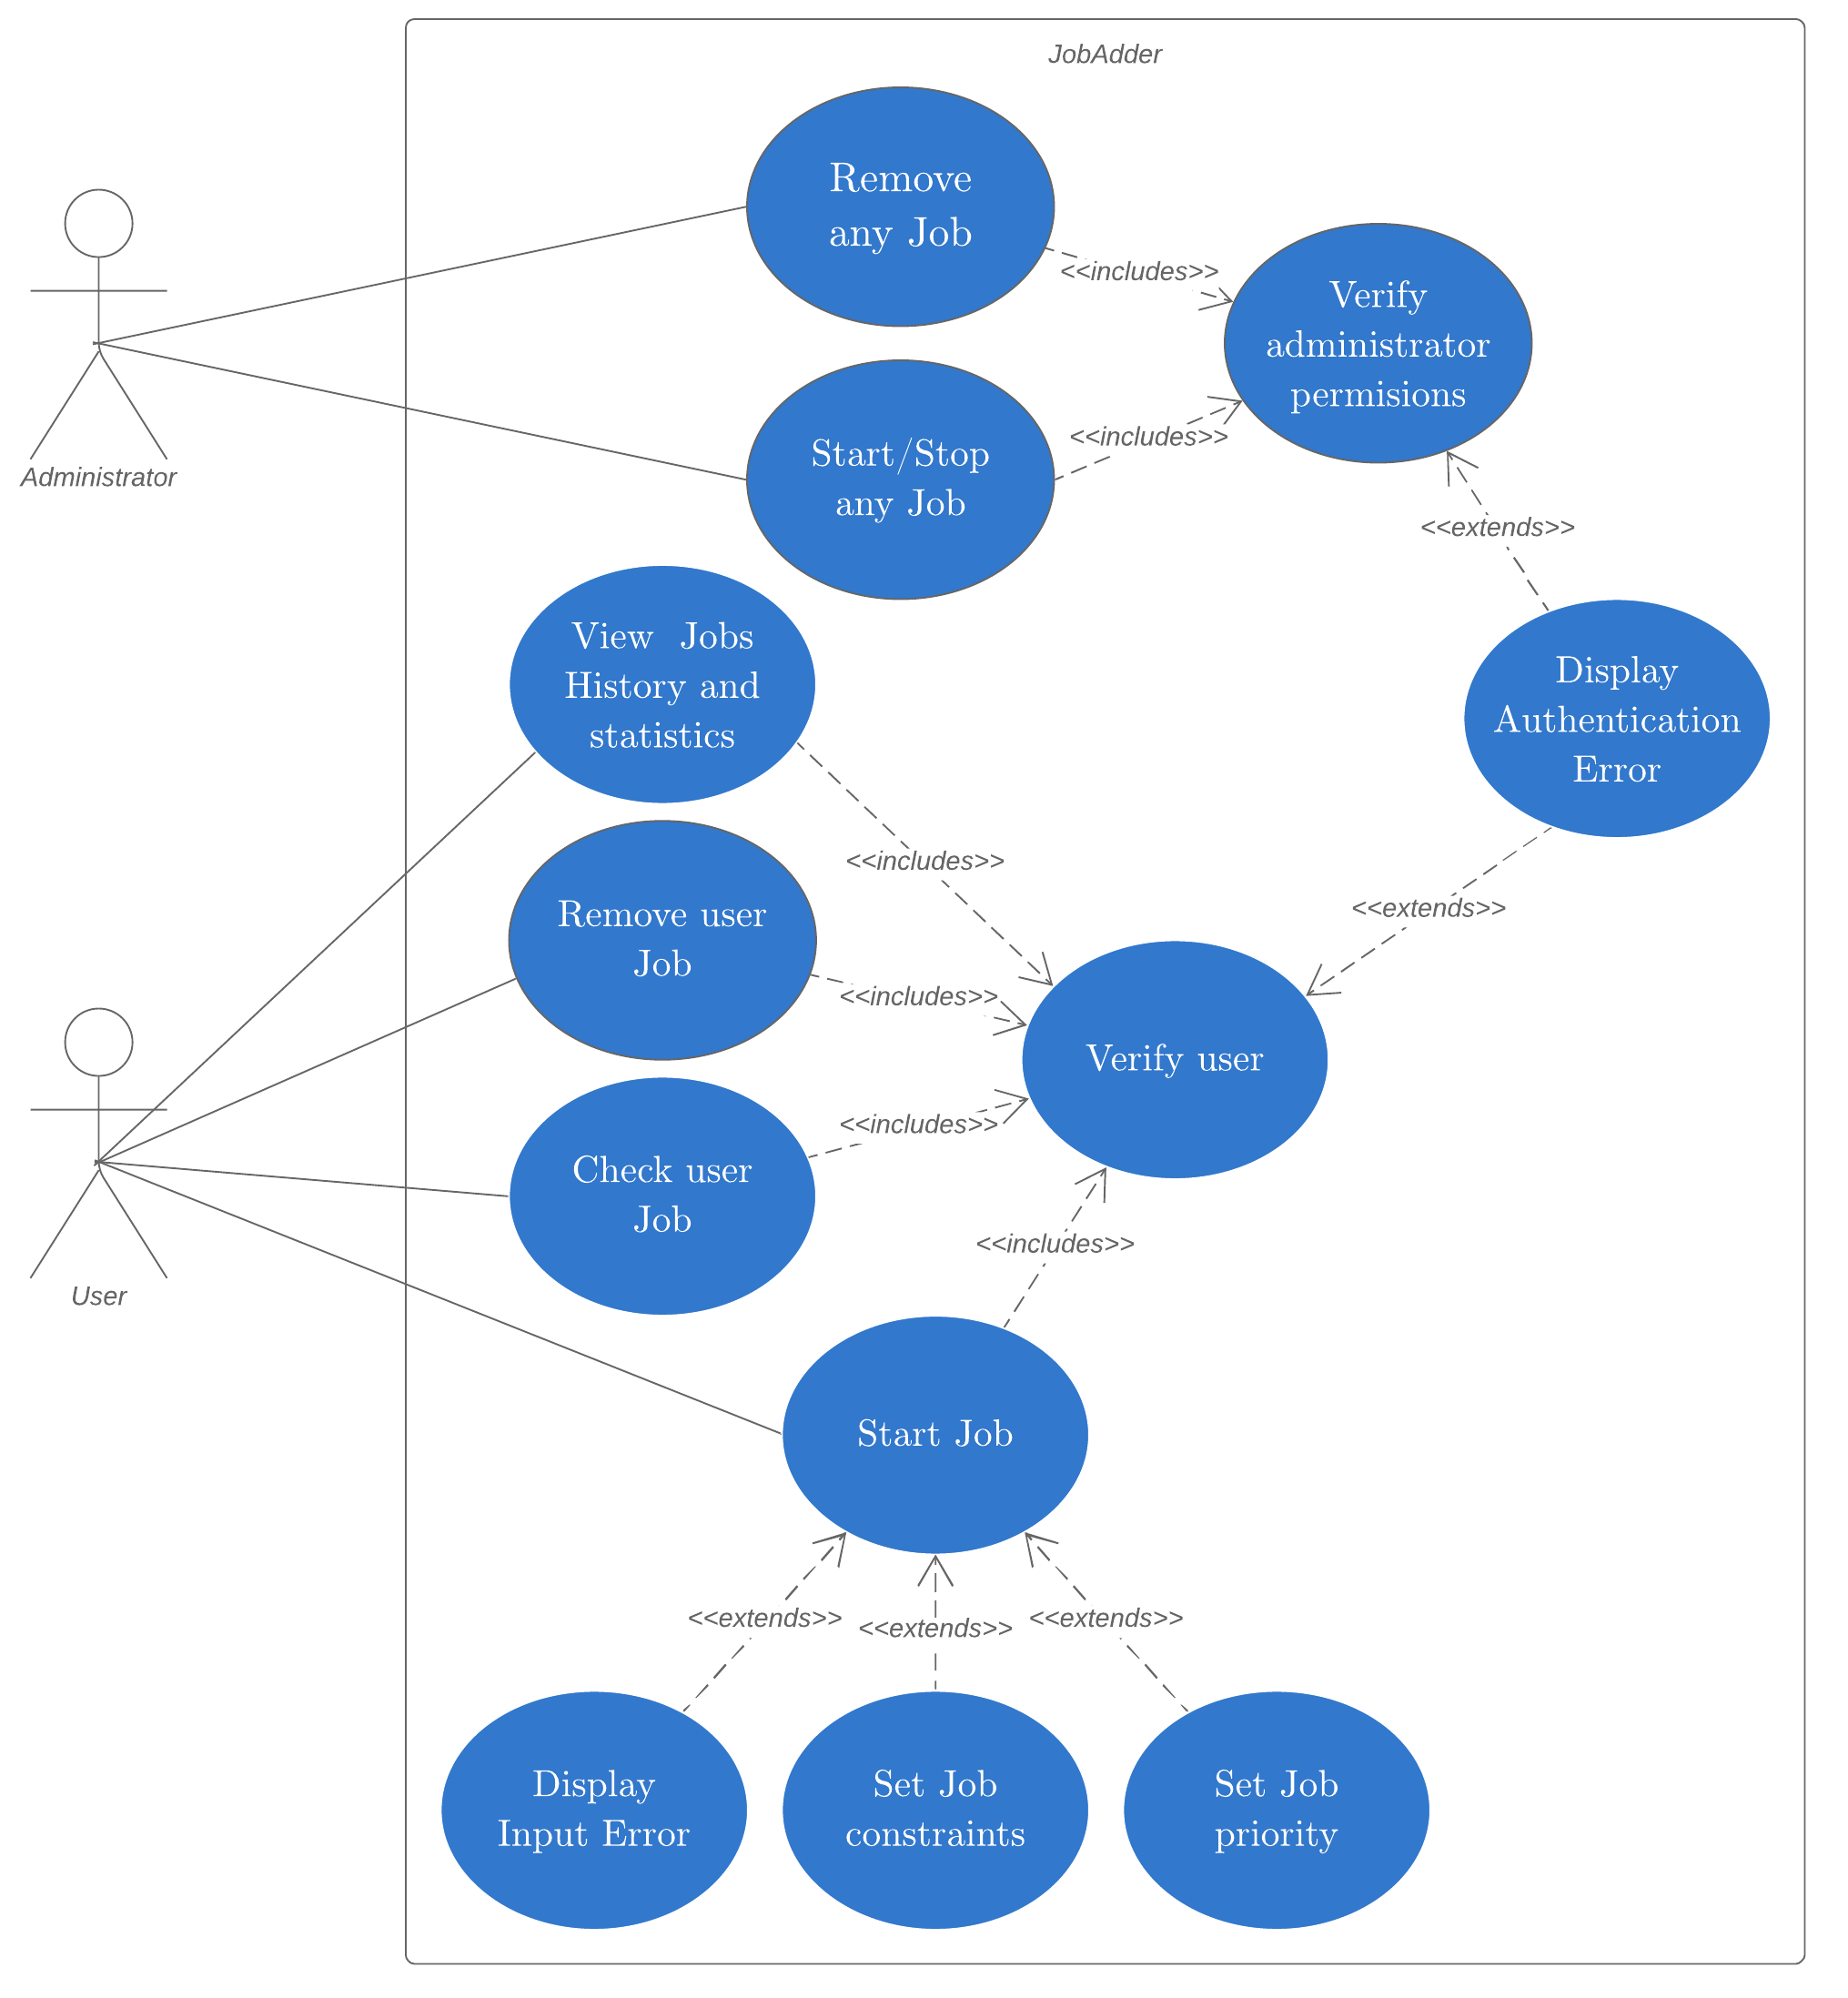
\includegraphics[width=\linewidth]{./system/systemmodel/images/usecasediagram.png}

\subsection{System Model}
\begin{figure}
  \subsubsection{Schedule new Job}
  \centering
  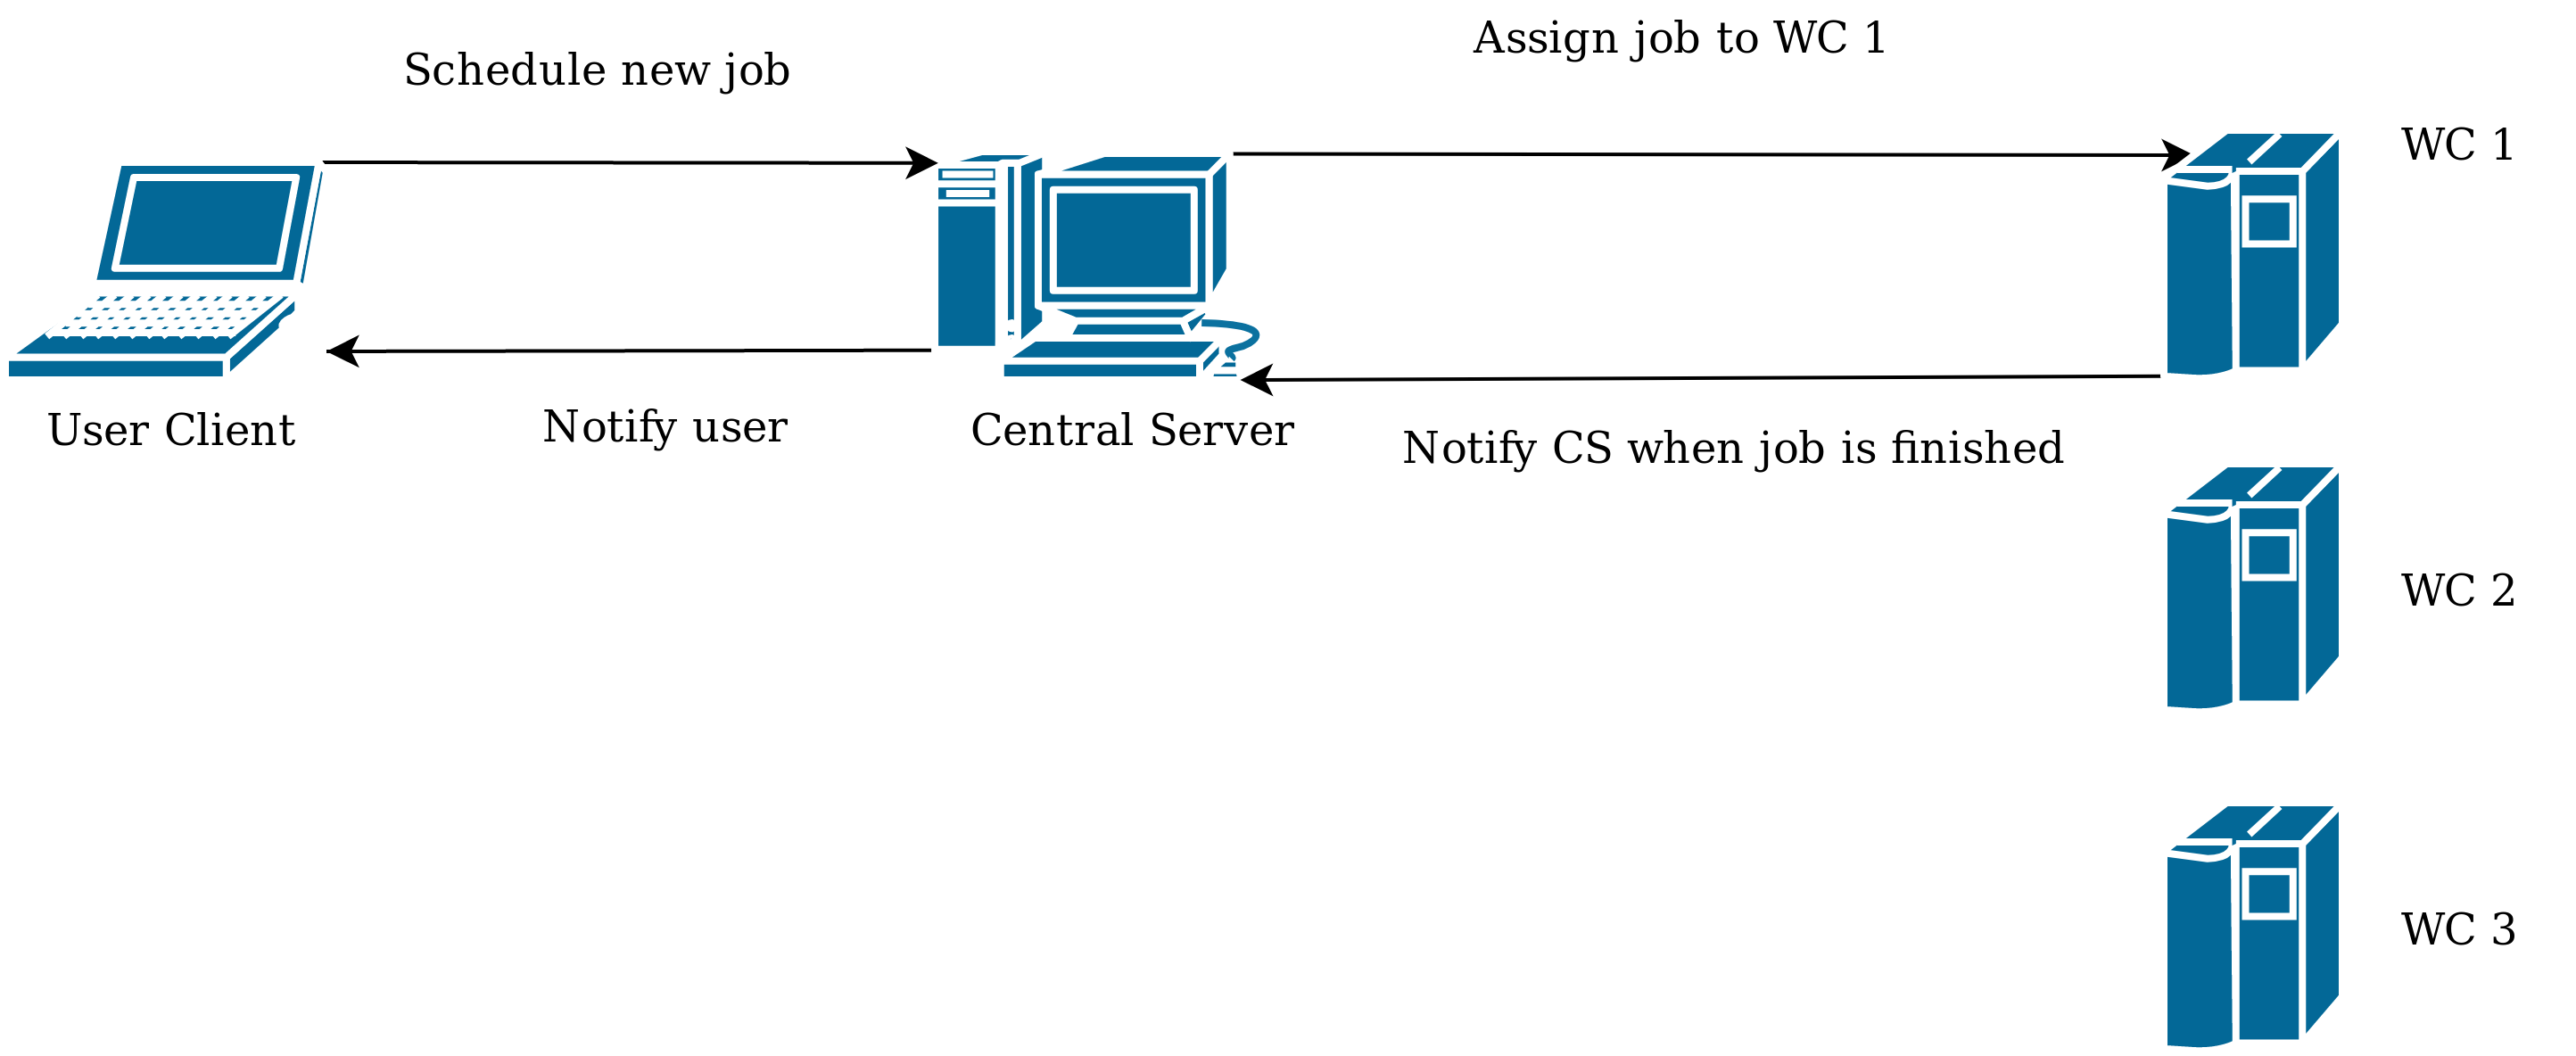
\includegraphics[width=\linewidth]{./system/systemmodel/images/schedulejob.png}
  \label{new-job}
  \caption{This diagram depicts how a user schedules a job, which the CS distributes to WC 1.
  In that case CS knows that there are enough resurces on WC 1 to execute users job.
  At the end the CS notifies the user that the job has finished.}
\end{figure}

\begin{figure}
  \subsubsection{Access a job}
  \centering
  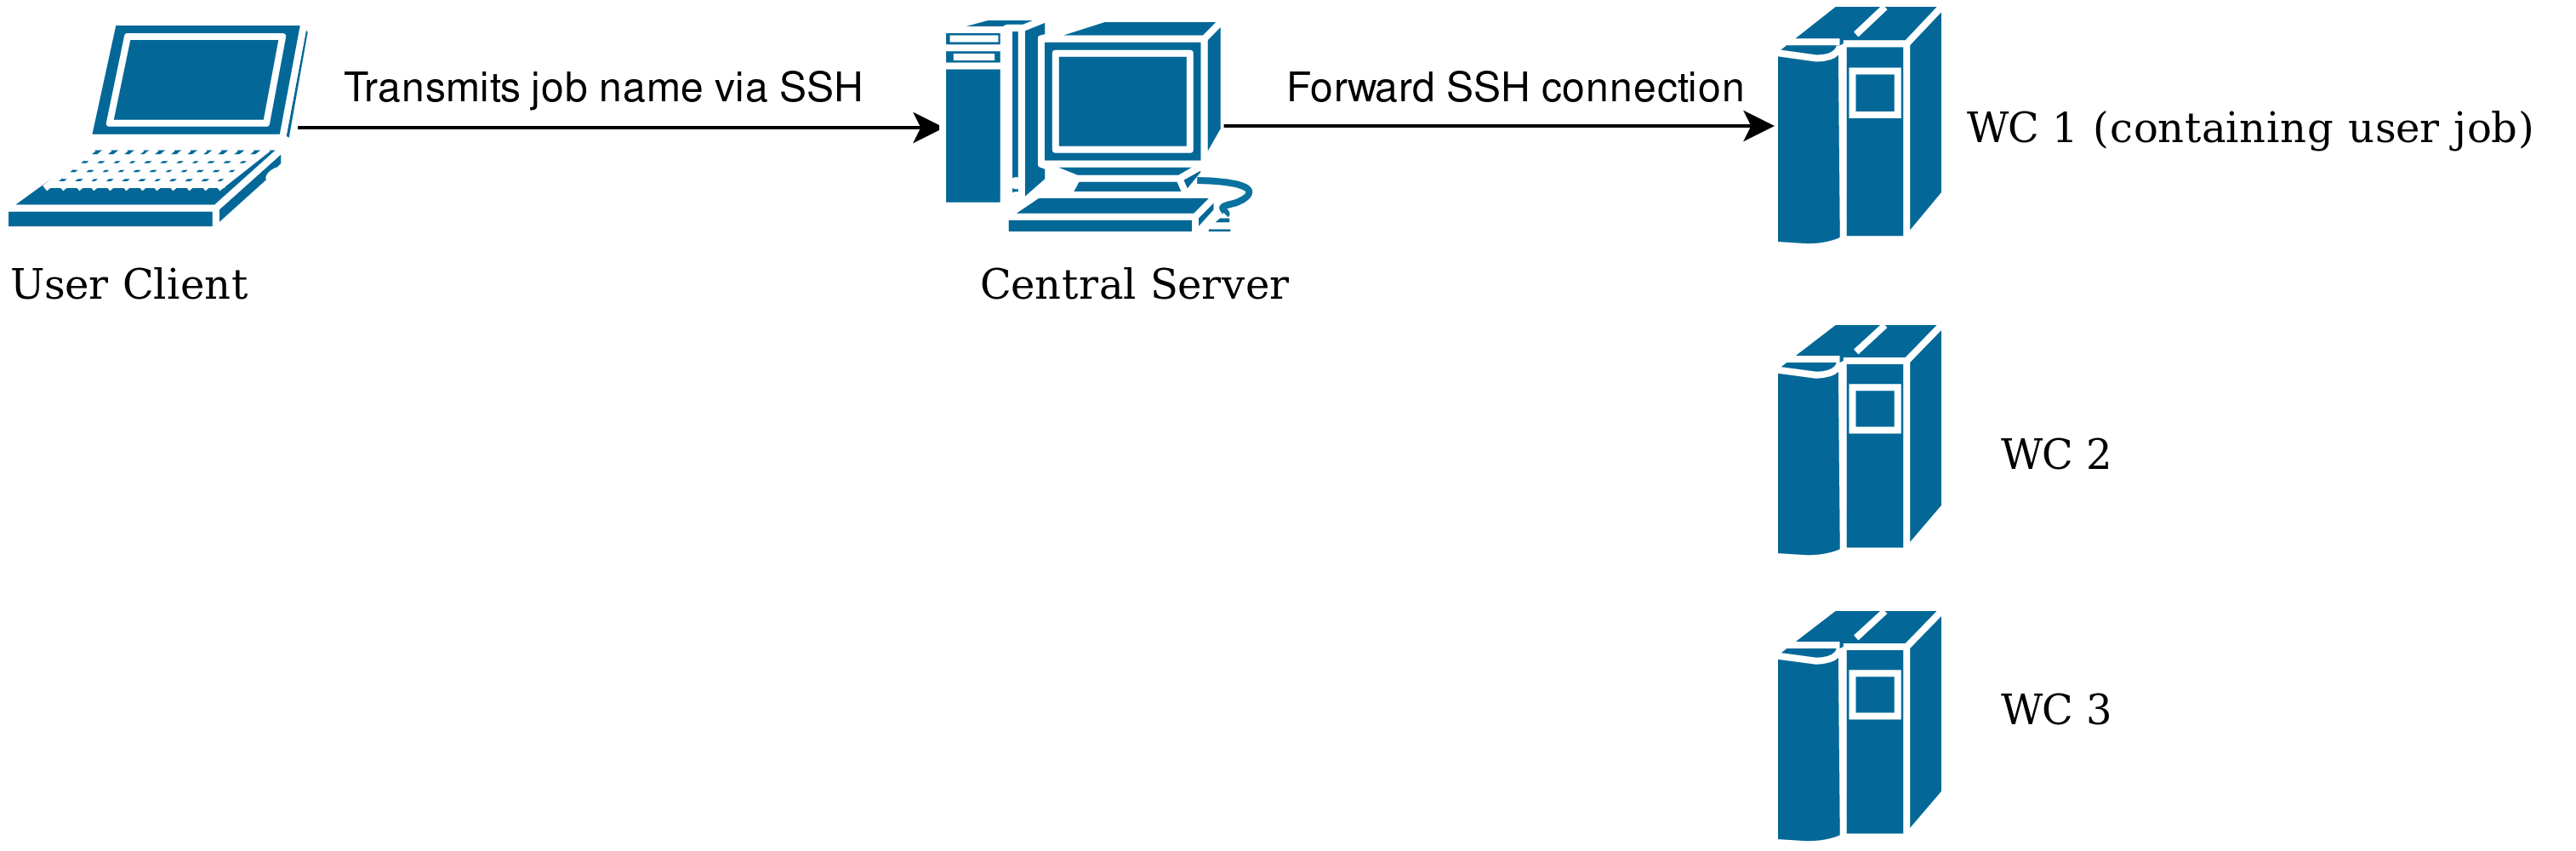
\includegraphics[width=\linewidth]{./system/systemmodel/images/accessjob.png}
  \label{access-job}
  \caption{This diagram depicts how a user accesses his job.
  The user has a job on one of the work machines that he wants to connect to.
  The user does not establish a direct connection with the WC.
  The user establishes an SSH connection to the server.
  This connection authenticates the user.
  It is also used to transmit the name of the job that the user wants to connect to.
  The server looks up which work machine the user's job is located on and forwards the SSH connection to that work machine.
  Finally, the SSH connection to the work machine is forwarded to the container with the user's job.}
\end{figure}

\begin{figure}
  \subsubsection{Get statistics}
  \centering
  
\includegraphics[width=0.5\linewidth]{./system/systemmodel/images/statistics.png}
  \label{statistics}
  \caption{This diagram depicts how a user accesses the statistics saved on the server.}
\end{figure}


\printunsrtglossaries
\end{document}


\newpage
\subsection{Use Case Diagram}
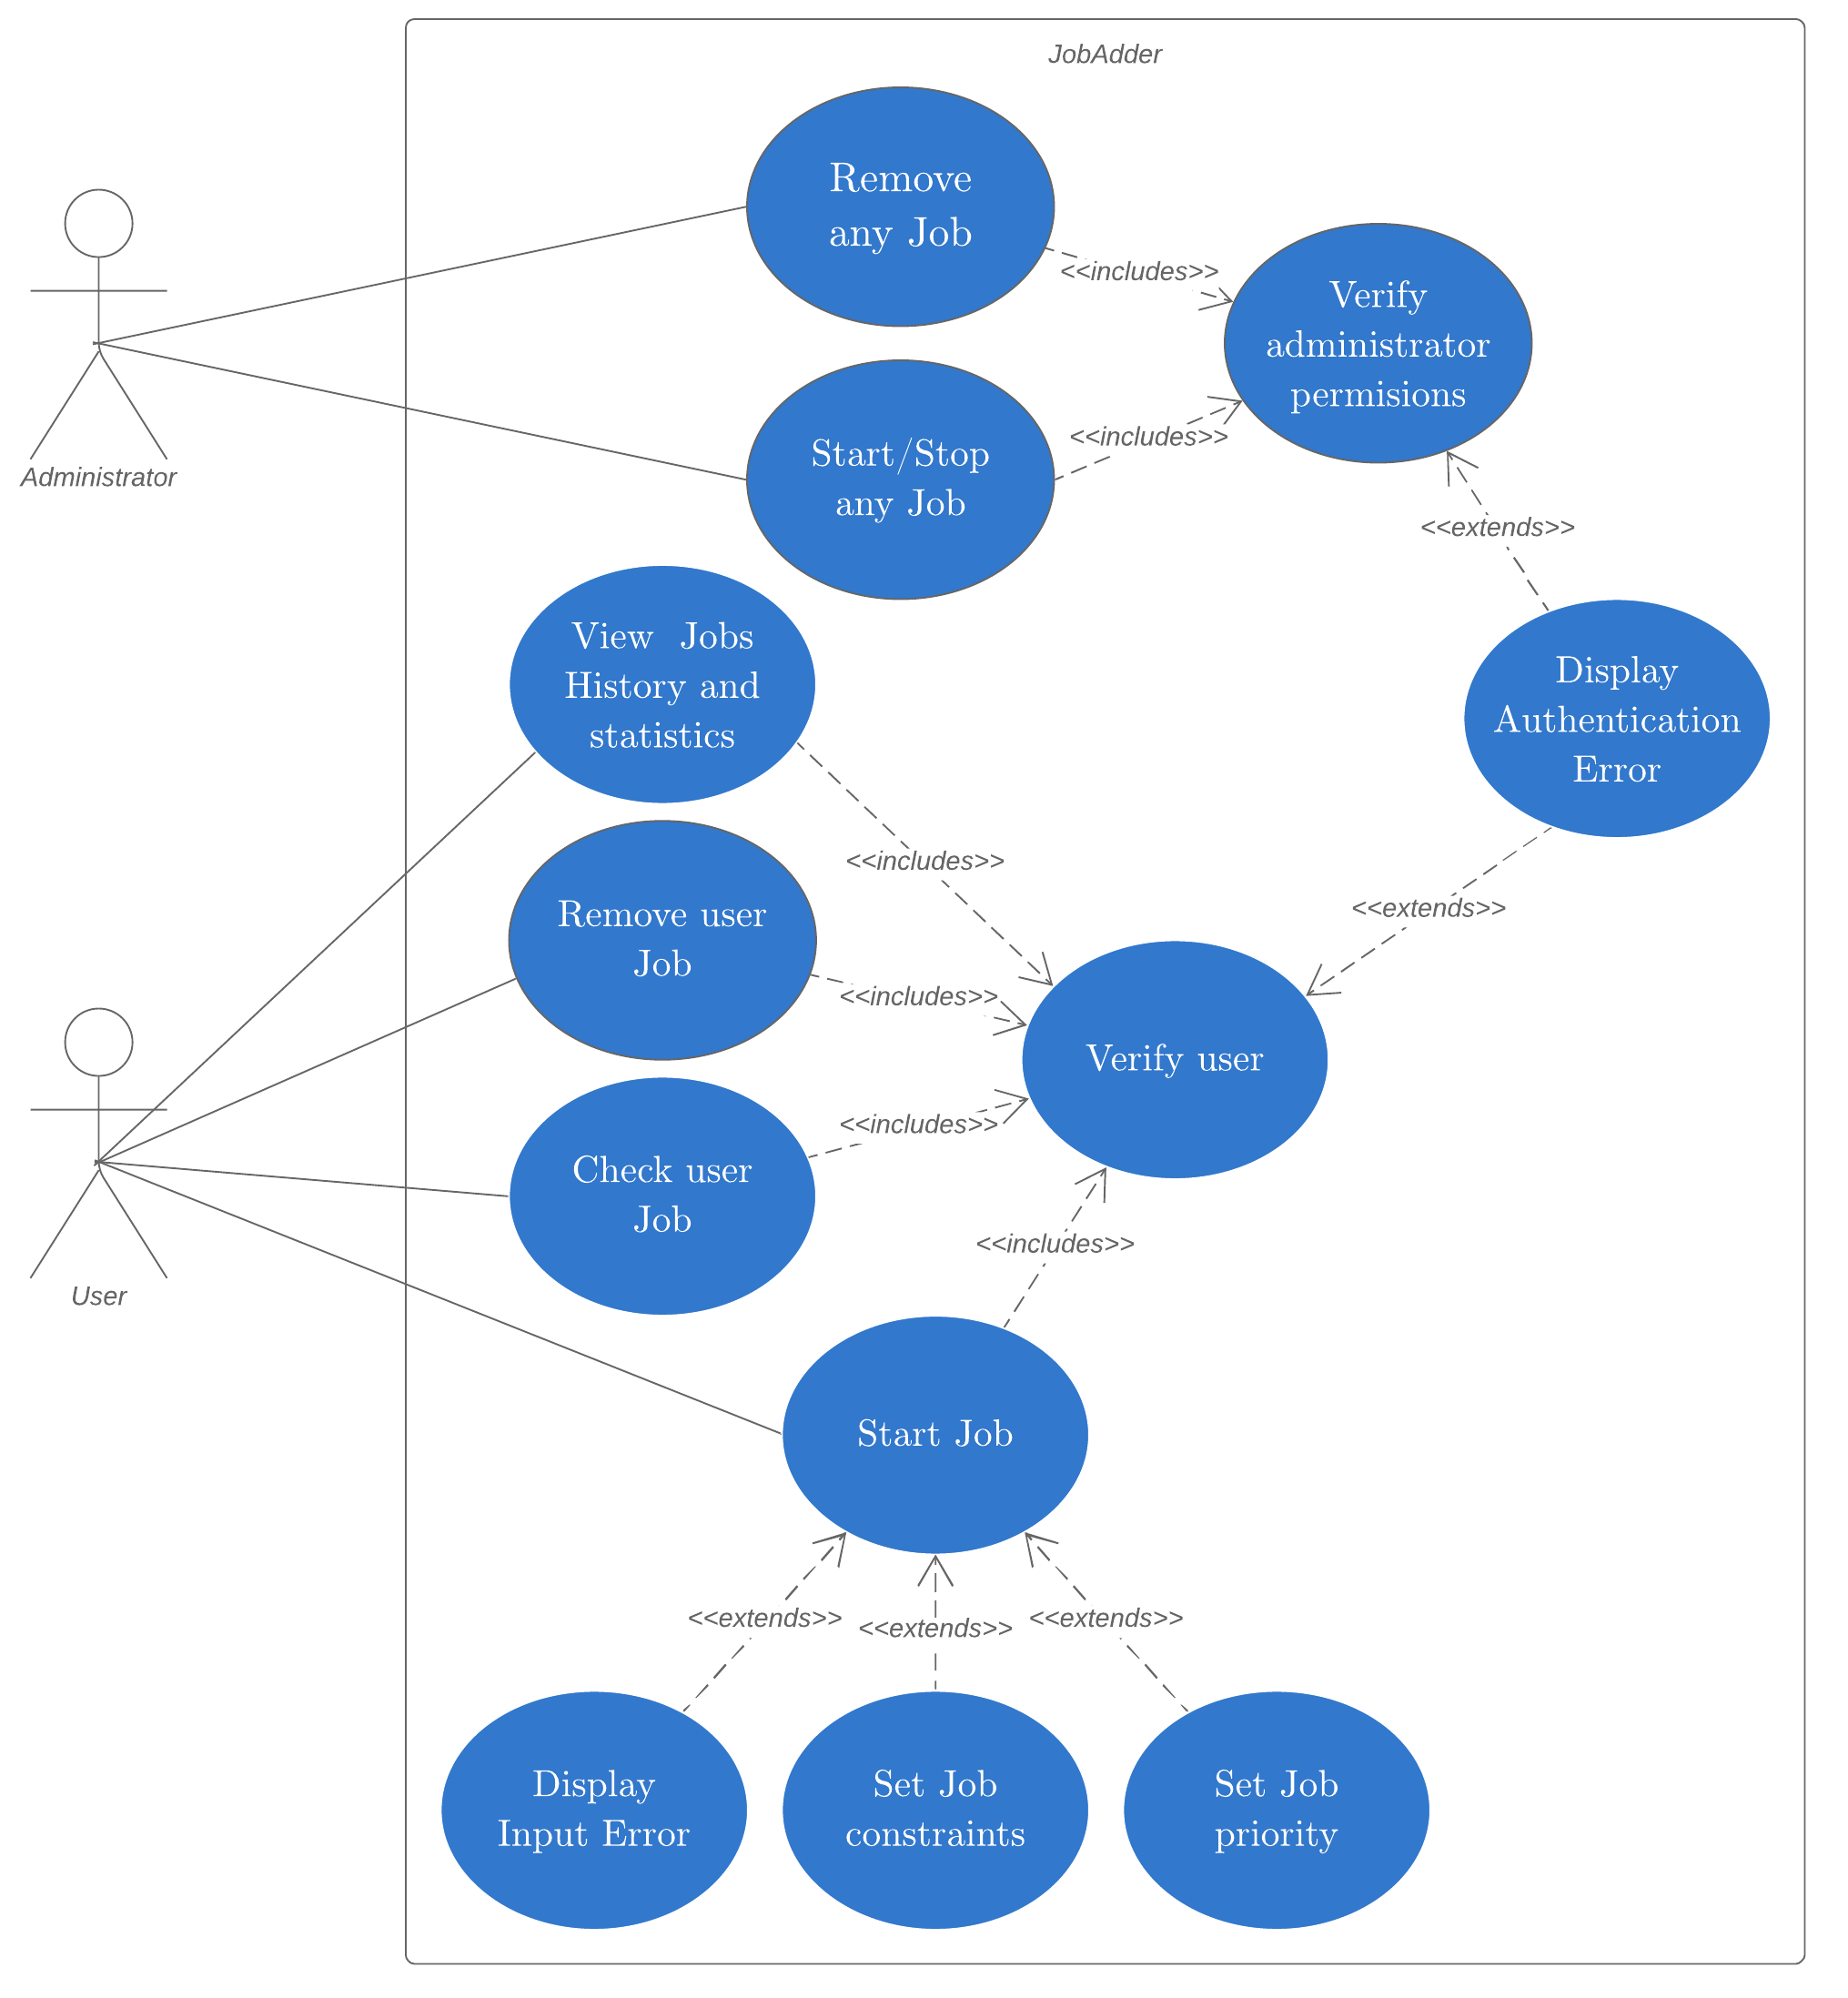
\includegraphics[width=\linewidth]{./system/systemmodel/images/usecasediagram.png}

\subsection{System Model}
\begin{figure}
  \subsubsection{Schedule new Job}
  \centering
  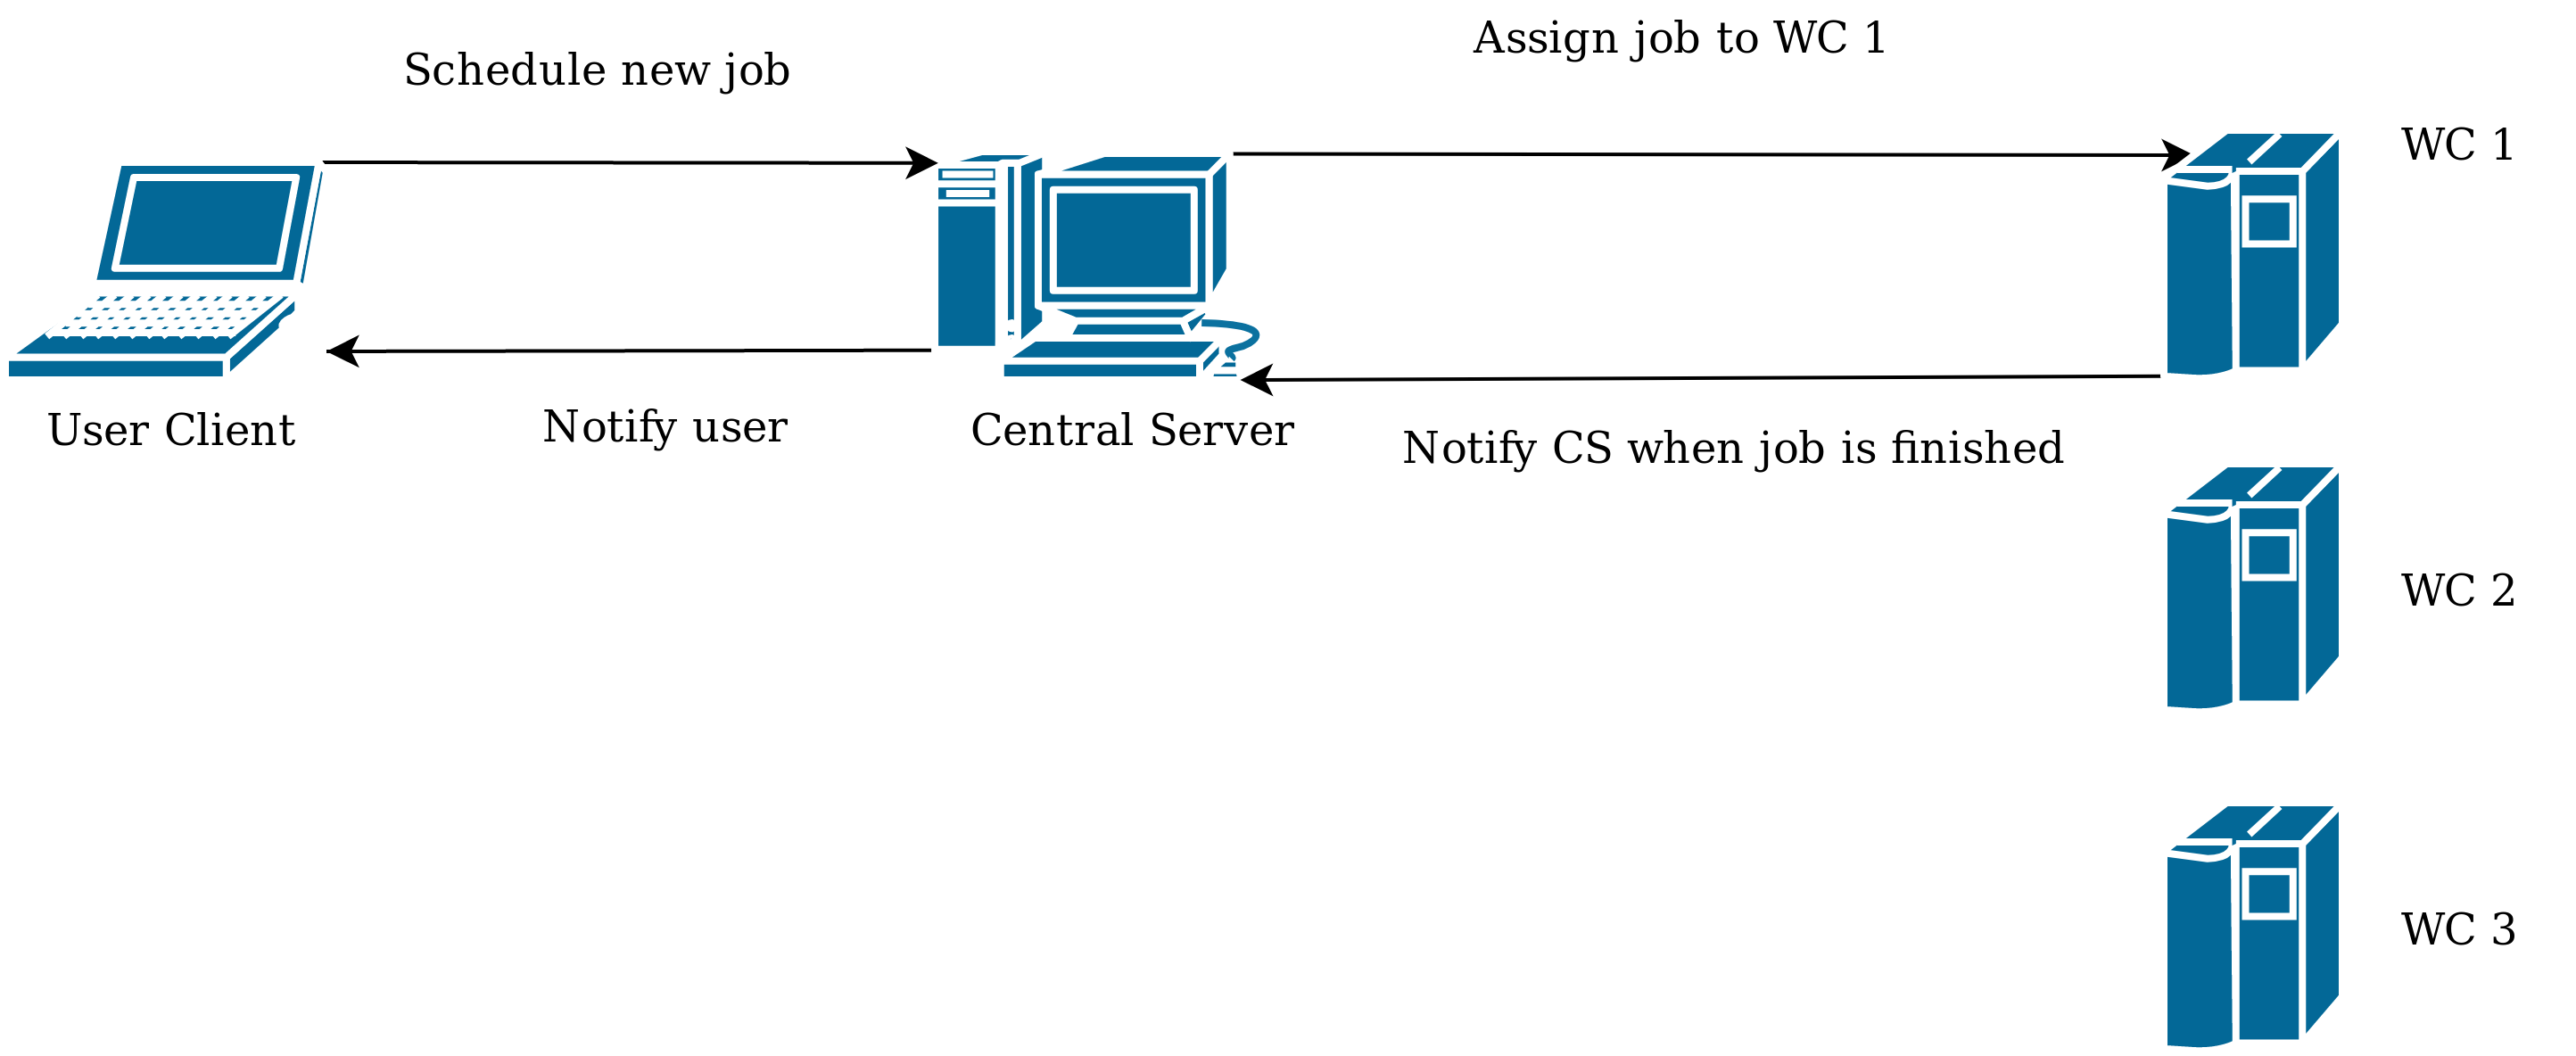
\includegraphics[width=\linewidth]{./system/systemmodel/images/schedulejob.png}
  \label{new-job}
  \caption{This diagram depicts how a user schedules a job, which the CS distributes to WC 1.
  In that case CS knows that there are enough resurces on WC 1 to execute users job.
  At the end the CS notifies the user that the job has finished.}
\end{figure}

\begin{figure}
  \subsubsection{Access a job}
  \centering
  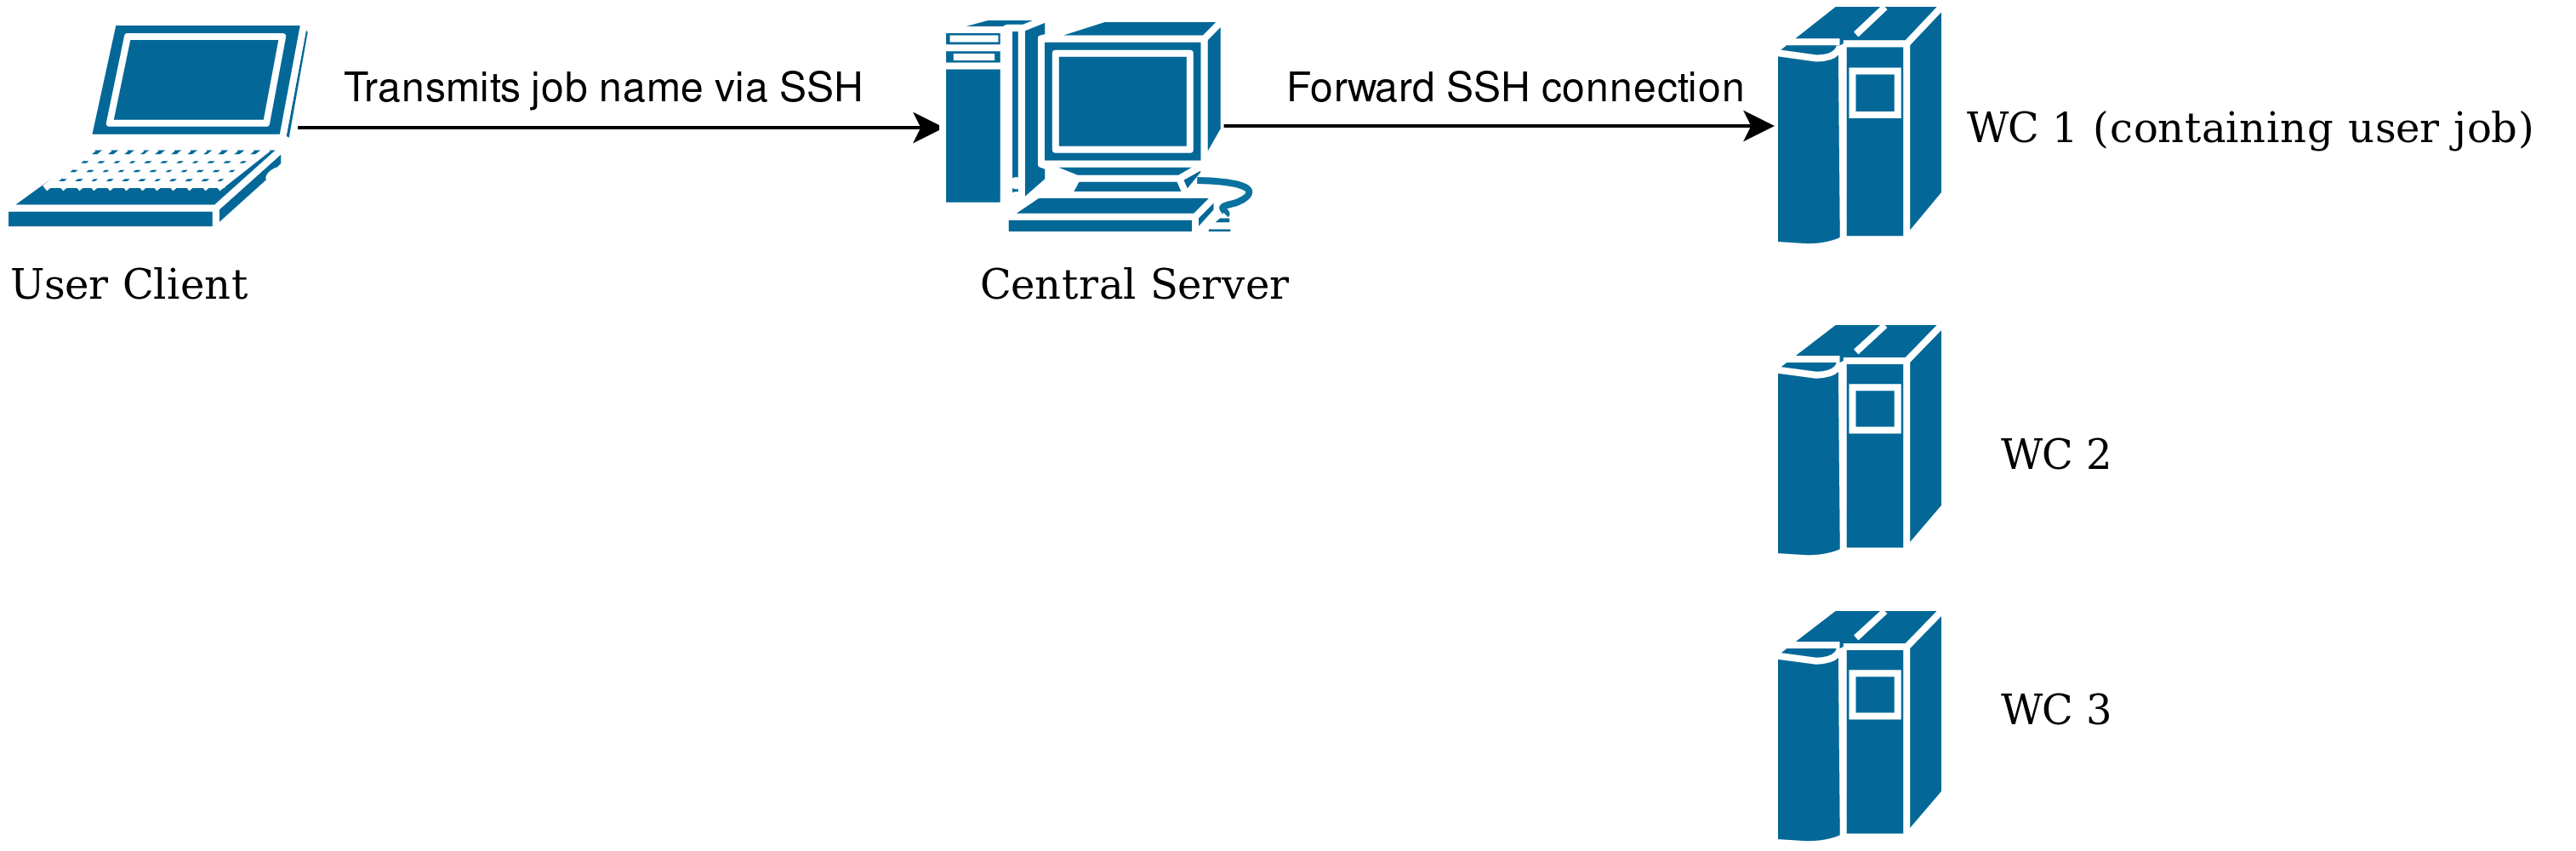
\includegraphics[width=\linewidth]{./system/systemmodel/images/accessjob.png}
  \label{access-job}
  \caption{This diagram depicts how a user accesses his job.
  The user has a job on one of the work machines that he wants to connect to.
  The user does not establish a direct connection with the WC.
  The user establishes an SSH connection to the server.
  This connection authenticates the user.
  It is also used to transmit the name of the job that the user wants to connect to.
  The server looks up which work machine the user's job is located on and forwards the SSH connection to that work machine.
  Finally, the SSH connection to the work machine is forwarded to the container with the user's job.}
\end{figure}

\begin{figure}
  \subsubsection{Get statistics}
  \centering
  
\includegraphics[width=0.5\linewidth]{./system/systemmodel/images/statistics.png}
  \label{statistics}
  \caption{This diagram depicts how a user accesses the statistics saved on the server.}
\end{figure}


\printunsrtglossaries
\end{document}

\newpage
\chapter{Product Environment}
  \section{User Client}
    \subsection{Hardware Requirements}
      \begin{itemize}
      \item A connection to the central server.
      \item 2 MB of storage space and an additional 100 MB per image.
      \end{itemize}
    \subsection{Software Requirements}
      \begin{itemize}
      \item Python 3.
    \end{itemize}

  \section{Central Server}
    \subsection{Hardware Requirements}
    \begin{itemize}
      \item 500 MB of storage space.
      \item 2 GB of RAM.
      \item One physical CPU core.
    \end{itemize}
    \subsection{Software Requirements}
    \begin{itemize}
      \item Linux Ubuntu 18.04 or newer, or CentOS 7.5 or newer.
      \item MySQL Database Server version 8.0 or newer.
      \item Linux kernel version 3.10 or higher.
      \item CS Docker engine 1.13, EE Deamon 17.03 and higher.
      \item Python 3.
    \end{itemize}

  \section{Working Machine Client}
    \subsection{Hardware Requirements}
      In addition to the hardware required to run a job, our worker client would need the following resources:
    \begin{itemize}
      \item A connection to a LAN.
      \item 4 GB of RAM.
      \item 3 GB of available disk space.
      \item Static IP Address.
    \end{itemize}
    \subsection{Software Requirements}
    \begin{itemize}
      \item Linux kernel version 3.10 or higher.
      \item CS Docker engine 1.13, EE Deamon 17.03 and higher.
      \item Python 3.
    \end{itemize}


\newpage
\subsection{Scheduling Algorithm}
This section describes how the central server distributes jobs to work machines: the \textit{scheduling algorithm}.
Put briefly, the scheduling algorithm takes a list of jobs and decides which ones to run on the available work machines.
The scheduling algorithm has the following goals:
\begin{itemize}
\item Keep work machines busy: there should be no idle work machines if there are pending jobs.
\item Consider job priorities: jobs with high priorities should be worked on first.
\item Consider time of job submission: jobs that were submitted first should be worked on first (if priorities are equal).
\end{itemize}
The scheduling algorithm operates under the following conditions:
\begin{itemize}
\item Jobs arrive at unforeseen times.
\item Time required to complete jobs is unknown.
\item Jobs cannot be transferred from one work machine to another.
\item Jobs cannot be canceled and restarted.
\item Job preemption is limited: if a job is paused it has to be kept in memory.
Note that memory includes swap files.
\item Some jobs cannot be paused due to software licensing restrictions.
\end{itemize}
The scheduling algorithm takes the following parameters as input:
\begin{itemize}
\item List of pending jobs.
\item List of running/paused jobs per work machine.
\item Amount of work machine specific resources: CPU threads, memory, etc.
These resources can typically be freed by pausing jobs.
\item Amount of work machine unspecific resources: software licenses.
Whether these resources can be freed by pausing jobs depends on the software.
\item Size of work machine swap files.
This resource is used exclusively for holding paused jobs.
It has no influence on running jobs.
\end{itemize}
The scheduling algorithm reevaluates which jobs to run every time a job finishes running or when a new job request arrives.
The scheduling algorithm assigns jobs to work machines as follows:
\begin{enumerate}
\item If there are pending urgent jobs:
Assign oldest urgent jobs to work machines until urgent jobs or resources run out.
Non-urgent running jobs will be paused if possible and necessary to run more urgent jobs.
\item If there are paused high-priority jobs:
Assign oldest paused high-priority jobs to work machines until paused high-priority jobs or resources run out.
Running jobs with equal or lower priority will be paused if possible and necessary to run more old paused high-priority jobs.
\item Repeat 2. for paused medium-priority jobs.
\item Repeat 2. for paused low-priority jobs.
\item If there are pending high-priority jobs:
Assign oldest paused high-priority jobs to work machines until paused high-priority jobs or resources run out.
Running jobs with equal or lower priority will be paused if possible and necessary to run the oldest available high-priority job.
\item Repeat 5. for pending medium-priority jobs.
\item Repeat 5. for pending low-priority jobs.
\end{enumerate}
\newpage
\newcommand{\jacommand}[3]{
\textsc{\LARGE{\textbf{#1}}}
\begin{itemize}
\item \textbf{Options:} #2
\item \textbf{Effect:} #3
\end{itemize}
}
\newcommand{\jaoptionheader}{\textsc{\textbf{Option descriptions:}}\newline\newline}
\newcommand{\jaoption}[3]{
\textbf{#1}
\begin{itemize}
\item \textbf{Short form:} #2
\item \textbf{Effect:} #3
\end{itemize}
}
\subsection{Command Line Interface}
All components of JobAdder are accessible through a command line interface (CLI).
The command line interface on a machine with JobAdder installed has the following structure:
\begin{equation}
\text{<component name> <command> <options> <targets>},
\end{equation}
where the \textit{component name} can be any one of the following:
\begin{itemize}
\item \textbf{jobadder} to access the \textit{user client}.
\item \textbf{jobcenter} to access the \textit{server}.
\item \textbf{jobworker} to access the \textit{worker client}.
\end{itemize}
Commands, options, and valid targets are and options are specified in the following sections.

Options can be added in the following ways:
\begin{itemize}
\item By supplying their names like "-{}-option\_x -{}-option\_y=2 -{}-option\_z".
\item By supplying their abbreviations like "-x -y 2 -z".
\item By supplying their abbreviations like "-xz -y 2".
\end{itemize}

The available \textit{commands} are generally specific to the used component.
Likewise, the available \textit{options} and \textit{targets} are generally specific to the commands of a used component.
However, some commands and options are shared between components or commands.

The JobAdder CLI only uses lower-case letters.
JobAdder CLI options override the values of configuration files.
If no command is given, the general help text for the given component is printed out.
\subsubsection{Shared Options}
\jaoption{config}{c}{Overrides the global configuration file with the given configuration file.}
\jaoption{detach}{d}{Detaches the execution of the given command from the command line.}
\jaoption{help}{h}{
Prints out a list of the available commands. 
When used in conjunction with a command:
prints out more detailed information on the given command and a list of the available options.}
\jaoption{verbose}{v}{
Determines the amount of information printed out.
If set to 2, detailed information is printed out.
If set to 1, only high-level information is printed out (default).
If set to 0, no information is printed out.}
\subsubsection{User Client}
\jacommand{add}
{gpu, mount, name, priority, server, ram, threads}
{Sends one or more job requests to the server.
If targets are Docker containers the job consists of simply running the container.
If targets are configuration files with a specified terminal command the job consists of running the specified terminal command.
Otherwise targets are interpreted as terminal commands}
\jaoptionheader
\jaoption{gpu}{g}{
If set to true, informs the server that the job requires a gpu.
If set to a string that can be interpreted as VRAM amount, informs the server that a GPU with this amount of VRAM is required for the job.
If set to a specific GPU model, informs the server that the job must be run on a machine with that GPU built in.
}
\jaoption{mount}{m}
{Directories that need to be mounted onto the Docker container that the job is running in.}
\jaoption{name}{n}
{Human-readable name of the job.
Defaults to user's name + job index}
\jaoption{priority}{p}
{Sets the priority of the job: urgent, high, medium, or low.
Defaults to medium.}
\jaoption{server}{s}
{Server to send the job request to.
Defaults to localhost.}
\jaoption{ram}{r}
{If set to a string that can be interpreted as RAM amount, informs the server that this amount of RAM is required for the job.}
\jaoption{threads}{t}
{If set to an integer, informs the server that this number of threads is required for the job.}
\jacommand{query}{user}
{Prints out information on running/queued/past jobs (specified by target).
In addition to the one below, options from add command can be used as constraints.}
\jaoptionheader
\jaoption{after}{a}{Only return jobs added after the given point in time.}
\jaoption{before}{b}{Only return jobs added before the given point in time.}
\jaoption{user}{u}{Filter query by user that added the job.}
\jacommand{stop}{None}{Stops the job with the specified name.}
\subsubsection{Server}
\jacommand{start}{None}{Starts an instance of the JobAdder server.}
\jacommand{stop}{None}{Stops instances of the JobAdder server.}
\subsubsection{Worker Client}
\jacommand{start}{server}{Starts an instance of the JobAdder worker client.}
\jaoptionheader
\jaoption{server}{s}
{Server to receive jobs from.
Defaults to localhost.}
\jacommand{stop}{None}{Stops instances of the JobAdder worker client.}

\newpage
\documentclass[a4paper,10pt]{scrreprt}
\usepackage[T1]{fontenc}
\usepackage[utf8]{inputenc}
\usepackage[nonumberlist,nopostdot]{glossaries-extra}     % provides glossary commands
\usepackage{graphicx}       % provides commands for including figures
\usepackage{amsmath}
\usepackage{float}
\usepackage{hyperref}

% Glossary needs to be before \begin{document}
\newglossaryentry{ID}
{
  name=ID,
  plural=IDs,
  description={
    An ID is a string of digits, english letters (both lower- and uppercase) and slashes '-'.
  }
}
\newglossaryentry{job status}
{
  name=job status,
  plural=job status,
  description={
    The status of a job can be:
    \begin{itemize}
      \item Queued - the job is waiting for a suitable work machine to become available.
      \item Running - the job is running on some work machine.
      \item Paused - the job has been running, but has been paused to allow for execution of other jobs.
      \item Done - the job has finished running.
      \item Killed - the job was forcefully stopped.
      \item Crashed - the work machine the job was running on shut down unexpectedly.
    \end{itemize}
  }
}
\newglossaryentry{job priority}
{
  name=job priority,
  plural=job priorities,
  description={
    The priority of a job can be one of the following (in ascending order):
    \begin{itemize}
      \item Low
      \item Medium
      \item High
      \item Urgent
    \end{itemize}
  }
}
\newglossaryentry{job}
{
  name=job,
  plural=jobs,
  description={
      A job in the context of JobAdder consists of the following:
      \begin{itemize}
        \item A unique job \gls{ID}.
        \item A program to be executed.
        \item A unix user who owns the job.
        \item \Gls{job priority}.
        \item Number of CPU threads needed for the execution of the program, an integer.
        \item Amount of RAM in megabytes needed for the execution of the program, an integer.
        \item Paths in the network storage needed for the application.
        \item One of:
        \begin{itemize}
          \item A Dockerfile providing instructions to build program environment.
          \item The name of predefined container environment, for ex. a base image from Docker Hub.
        \end{itemize}
     \end{itemize}
  }
}
\newglossaryentry{timestamp}
{
  name=timestamp,
  plural=timestamps,
  description={
    A timestamp is a combination of the date and time of a particular point in time.
    It has the following format: "YYYY-DD-MM HH:MM:SS".
  }
}
\newglossaryentry{administrator}
{
  name=administrator,
  plural=administrators,
  description={
    An administrator is a user who can terminate queued and running jobs from all users.
  }
}
\newglossaryentry{UID}
{
  name=UID,
  plural=UIDs,
  description={
    A UID (user identifier) is a number assigned by Linux to each user on the system.
  }
}
\newglossaryentry{GID}
{
  name=GID,
  plural=GIDs,
  description={
    A GID (group identifier) is a number assigned by Linux to each group on the system.
  }
}
\newglossaryentry{Dockerfile}
{
  name=Dockerfile,
  plural=Dockerfiles,
  description={
     A Dockerfile is a text document that contains all the commands a user could call on the
     command line to assemble an image.
  }
}


%opening
\title{JobAdder: Requirements}
\author{Johannes Gäßler \and  Ilia Bozhinov \and Nikola Tzotchev \and Malik Bouguila \and Jamil Bagga}

\begin{document}

\maketitle
\tableofcontents
\newpage

\section{Introduction}
The JobAdder project enables users to remotely execute resource-intensive tasks on a dedicated cluster of work machines.
Tasks are being distributed to work machines automatically.\newline
The distribution reduces task execution times and peak system loads by better utilizing the available hardware.
In addition, JobAdder provides tools to inspect the state of the whole system and display statistics about user activity.
\section{Purpose}
  \subsection{Product Goal}
    JobAdder aims to facilitate and accelerate the execution of computationally
    expensive jobs in a cluster of work machines.

    Currently, users need to access every single work machine manually in order to
    distribute their jobs over them. Even more problems arise when a group of users
    is involved. In that case, users have to look for the work machine with the
    least amount of work and add their job to it.
   
    JobAdder addresses and solves these problems. With JobAdder, users are able to
    send their jobs to a central server in order to evenly distribute them over
    suitable work machines without having to look for them manually. So if there is
    enough workload (which is usually the case), no machine remains idle unless it
    is forced to.

    Jobadder also aims to make task scheduling more user-friendly. A user does not
    have to keep checking the state of their job, they will be notified once the job
    is done. Nor does a user have to wait for an idle machine in order to queue a
    job, the central server saves them up and runs them once it is possible. There
    is also more insight into the whole system by providing statistics about user
    activity, currently running jobs, past jobs and queued jobs.
   
    Users can set priorities for their jobs so that jobs with high priority will be
    executed before jobs with low priority. Urgent jobs are immediately executed by
    pausing jobs with the lowest priority, so a user is not required to pause or
    cancel low-priority jobs manually. The scheduling algorithm also guarantees that
    every job is eventually run by automatically increasing it's priority over time.

  \subsection{Target Audience}
    The target audience mostly consists of groups of users with access to several
    work machines. This includes, companies, academic institutions and computing
    centers. These users usually need remote machines to run their jobs due to high
    hardware requirements.
   
    JobAdder helps them use their hardware more efficiently by adding an abstraction
    layer between the user and the work machines that are running the user's jobs.
\documentclass[a4paper,10pt]{scrreprt}
\usepackage[T1]{fontenc}
\usepackage[utf8]{inputenc}
\usepackage[nonumberlist,nopostdot]{glossaries-extra}     % provides glossary commands
\usepackage{graphicx}       % provides commands for including figures
\usepackage{amsmath}
\usepackage{float}
\usepackage{hyperref}

% Glossary needs to be before \begin{document}
\newglossaryentry{ID}
{
  name=ID,
  plural=IDs,
  description={
    An ID is a string of digits, english letters (both lower- and uppercase) and slashes '-'.
  }
}
\newglossaryentry{job status}
{
  name=job status,
  plural=job status,
  description={
    The status of a job can be:
    \begin{itemize}
      \item Queued - the job is waiting for a suitable work machine to become available.
      \item Running - the job is running on some work machine.
      \item Paused - the job has been running, but has been paused to allow for execution of other jobs.
      \item Done - the job has finished running.
      \item Killed - the job was forcefully stopped.
      \item Crashed - the work machine the job was running on shut down unexpectedly.
    \end{itemize}
  }
}
\newglossaryentry{job priority}
{
  name=job priority,
  plural=job priorities,
  description={
    The priority of a job can be one of the following (in ascending order):
    \begin{itemize}
      \item Low
      \item Medium
      \item High
      \item Urgent
    \end{itemize}
  }
}
\newglossaryentry{job}
{
  name=job,
  plural=jobs,
  description={
      A job in the context of JobAdder consists of the following:
      \begin{itemize}
        \item A unique job \gls{ID}.
        \item A program to be executed.
        \item A unix user who owns the job.
        \item \Gls{job priority}.
        \item Number of CPU threads needed for the execution of the program, an integer.
        \item Amount of RAM in megabytes needed for the execution of the program, an integer.
        \item Paths in the network storage needed for the application.
        \item One of:
        \begin{itemize}
          \item A Dockerfile providing instructions to build program environment.
          \item The name of predefined container environment, for ex. a base image from Docker Hub.
        \end{itemize}
     \end{itemize}
  }
}
\newglossaryentry{timestamp}
{
  name=timestamp,
  plural=timestamps,
  description={
    A timestamp is a combination of the date and time of a particular point in time.
    It has the following format: "YYYY-DD-MM HH:MM:SS".
  }
}
\newglossaryentry{administrator}
{
  name=administrator,
  plural=administrators,
  description={
    An administrator is a user who can terminate queued and running jobs from all users.
  }
}
\newglossaryentry{UID}
{
  name=UID,
  plural=UIDs,
  description={
    A UID (user identifier) is a number assigned by Linux to each user on the system.
  }
}
\newglossaryentry{GID}
{
  name=GID,
  plural=GIDs,
  description={
    A GID (group identifier) is a number assigned by Linux to each group on the system.
  }
}
\newglossaryentry{Dockerfile}
{
  name=Dockerfile,
  plural=Dockerfiles,
  description={
     A Dockerfile is a text document that contains all the commands a user could call on the
     command line to assemble an image.
  }
}


%opening
\title{JobAdder: Requirements}
\author{Johannes Gäßler \and  Ilia Bozhinov \and Nikola Tzotchev \and Malik Bouguila \and Jamil Bagga}

\begin{document}

\maketitle
\tableofcontents
\newpage

\section{Introduction}
The JobAdder project enables users to remotely execute resource-intensive tasks on a dedicated cluster of work machines.
Tasks are being distributed to work machines automatically.\newline
The distribution reduces task execution times and peak system loads by better utilizing the available hardware.
In addition, JobAdder provides tools to inspect the state of the whole system and display statistics about user activity.
\section{Purpose}
  \subsection{Product Goal}
    JobAdder aims to facilitate and accelerate the execution of computationally
    expensive jobs in a cluster of work machines.

    Currently, users need to access every single work machine manually in order to
    distribute their jobs over them. Even more problems arise when a group of users
    is involved. In that case, users have to look for the work machine with the
    least amount of work and add their job to it.
   
    JobAdder addresses and solves these problems. With JobAdder, users are able to
    send their jobs to a central server in order to evenly distribute them over
    suitable work machines without having to look for them manually. So if there is
    enough workload (which is usually the case), no machine remains idle unless it
    is forced to.

    Jobadder also aims to make task scheduling more user-friendly. A user does not
    have to keep checking the state of their job, they will be notified once the job
    is done. Nor does a user have to wait for an idle machine in order to queue a
    job, the central server saves them up and runs them once it is possible. There
    is also more insight into the whole system by providing statistics about user
    activity, currently running jobs, past jobs and queued jobs.
   
    Users can set priorities for their jobs so that jobs with high priority will be
    executed before jobs with low priority. Urgent jobs are immediately executed by
    pausing jobs with the lowest priority, so a user is not required to pause or
    cancel low-priority jobs manually. The scheduling algorithm also guarantees that
    every job is eventually run by automatically increasing it's priority over time.

  \subsection{Target Audience}
    The target audience mostly consists of groups of users with access to several
    work machines. This includes, companies, academic institutions and computing
    centers. These users usually need remote machines to run their jobs due to high
    hardware requirements.
   
    JobAdder helps them use their hardware more efficiently by adding an abstraction
    layer between the user and the work machines that are running the user's jobs.
\documentclass[a4paper,10pt]{scrreprt}
\usepackage[T1]{fontenc}
\usepackage[utf8]{inputenc}
\usepackage[nonumberlist,nopostdot]{glossaries-extra}     % provides glossary commands
\usepackage{graphicx}       % provides commands for including figures
\usepackage{amsmath}
\usepackage{float}
\usepackage{hyperref}

% Glossary needs to be before \begin{document}
\input{customer/glossary}

%opening
\title{JobAdder: Requirements}
\author{Johannes Gäßler \and  Ilia Bozhinov \and Nikola Tzotchev \and Malik Bouguila \and Jamil Bagga}

\begin{document}

\maketitle
\tableofcontents
\newpage

\input{customer/introduction}
\input{customer/goals}
\input{customer/main}
\input{customer/product-environment}
\input{customer/scheduling-algorithm}
\input{customer/cli}
\input{system/main}

\newpage
\input{system/systemmodel/use-case-diagram}
\input{system/systemmodel/system-model.tex}

\printunsrtglossaries
\end{document}

\chapter{Product Environment}
  \section{User Client}
    \subsection{Hardware Requirements}
      \begin{itemize}
      \item A connection to the central server.
      \item 2 MB of storage space and an additional 100 MB per image.
      \end{itemize}
    \subsection{Software Requirements}
      \begin{itemize}
      \item Python 3.
    \end{itemize}

  \section{Central Server}
    \subsection{Hardware Requirements}
    \begin{itemize}
      \item 500 MB of storage space.
      \item 2 GB of RAM.
      \item One physical CPU core.
    \end{itemize}
    \subsection{Software Requirements}
    \begin{itemize}
      \item Linux Ubuntu 18.04 or newer, or CentOS 7.5 or newer.
      \item MySQL Database Server version 8.0 or newer.
      \item Linux kernel version 3.10 or higher.
      \item CS Docker engine 1.13, EE Deamon 17.03 and higher.
      \item Python 3.
    \end{itemize}

  \section{Working Machine Client}
    \subsection{Hardware Requirements}
      In addition to the hardware required to run a job, our worker client would need the following resources:
    \begin{itemize}
      \item A connection to a LAN.
      \item 4 GB of RAM.
      \item 3 GB of available disk space.
      \item Static IP Address.
    \end{itemize}
    \subsection{Software Requirements}
    \begin{itemize}
      \item Linux kernel version 3.10 or higher.
      \item CS Docker engine 1.13, EE Deamon 17.03 and higher.
      \item Python 3.
    \end{itemize}


\subsection{Scheduling Algorithm}
This section describes how the central server distributes jobs to work machines: the \textit{scheduling algorithm}.
Put briefly, the scheduling algorithm takes a list of jobs and decides which ones to run on the available work machines.
The scheduling algorithm has the following goals:
\begin{itemize}
\item Keep work machines busy: there should be no idle work machines if there are pending jobs.
\item Consider job priorities: jobs with high priorities should be worked on first.
\item Consider time of job submission: jobs that were submitted first should be worked on first (if priorities are equal).
\end{itemize}
The scheduling algorithm operates under the following conditions:
\begin{itemize}
\item Jobs arrive at unforeseen times.
\item Time required to complete jobs is unknown.
\item Jobs cannot be transferred from one work machine to another.
\item Jobs cannot be canceled and restarted.
\item Job preemption is limited: if a job is paused it has to be kept in memory.
Note that memory includes swap files.
\item Some jobs cannot be paused due to software licensing restrictions.
\end{itemize}
The scheduling algorithm takes the following parameters as input:
\begin{itemize}
\item List of pending jobs.
\item List of running/paused jobs per work machine.
\item Amount of work machine specific resources: CPU threads, memory, etc.
These resources can typically be freed by pausing jobs.
\item Amount of work machine unspecific resources: software licenses.
Whether these resources can be freed by pausing jobs depends on the software.
\item Size of work machine swap files.
This resource is used exclusively for holding paused jobs.
It has no influence on running jobs.
\end{itemize}
The scheduling algorithm reevaluates which jobs to run every time a job finishes running or when a new job request arrives.
The scheduling algorithm assigns jobs to work machines as follows:
\begin{enumerate}
\item If there are pending urgent jobs:
Assign oldest urgent jobs to work machines until urgent jobs or resources run out.
Non-urgent running jobs will be paused if possible and necessary to run more urgent jobs.
\item If there are paused high-priority jobs:
Assign oldest paused high-priority jobs to work machines until paused high-priority jobs or resources run out.
Running jobs with equal or lower priority will be paused if possible and necessary to run more old paused high-priority jobs.
\item Repeat 2. for paused medium-priority jobs.
\item Repeat 2. for paused low-priority jobs.
\item If there are pending high-priority jobs:
Assign oldest paused high-priority jobs to work machines until paused high-priority jobs or resources run out.
Running jobs with equal or lower priority will be paused if possible and necessary to run the oldest available high-priority job.
\item Repeat 5. for pending medium-priority jobs.
\item Repeat 5. for pending low-priority jobs.
\end{enumerate}
\newcommand{\jacommand}[3]{
\textsc{\LARGE{\textbf{#1}}}
\begin{itemize}
\item \textbf{Options:} #2
\item \textbf{Effect:} #3
\end{itemize}
}
\newcommand{\jaoptionheader}{\textsc{\textbf{Option descriptions:}}\newline\newline}
\newcommand{\jaoption}[3]{
\textbf{#1}
\begin{itemize}
\item \textbf{Short form:} #2
\item \textbf{Effect:} #3
\end{itemize}
}
\subsection{Command Line Interface}
All components of JobAdder are accessible through a command line interface (CLI).
The command line interface on a machine with JobAdder installed has the following structure:
\begin{equation}
\text{<component name> <command> <options> <targets>},
\end{equation}
where the \textit{component name} can be any one of the following:
\begin{itemize}
\item \textbf{jobadder} to access the \textit{user client}.
\item \textbf{jobcenter} to access the \textit{server}.
\item \textbf{jobworker} to access the \textit{worker client}.
\end{itemize}
Commands, options, and valid targets are and options are specified in the following sections.

Options can be added in the following ways:
\begin{itemize}
\item By supplying their names like "-{}-option\_x -{}-option\_y=2 -{}-option\_z".
\item By supplying their abbreviations like "-x -y 2 -z".
\item By supplying their abbreviations like "-xz -y 2".
\end{itemize}

The available \textit{commands} are generally specific to the used component.
Likewise, the available \textit{options} and \textit{targets} are generally specific to the commands of a used component.
However, some commands and options are shared between components or commands.

The JobAdder CLI only uses lower-case letters.
JobAdder CLI options override the values of configuration files.
If no command is given, the general help text for the given component is printed out.
\subsubsection{Shared Options}
\jaoption{config}{c}{Overrides the global configuration file with the given configuration file.}
\jaoption{detach}{d}{Detaches the execution of the given command from the command line.}
\jaoption{help}{h}{
Prints out a list of the available commands. 
When used in conjunction with a command:
prints out more detailed information on the given command and a list of the available options.}
\jaoption{verbose}{v}{
Determines the amount of information printed out.
If set to 2, detailed information is printed out.
If set to 1, only high-level information is printed out (default).
If set to 0, no information is printed out.}
\subsubsection{User Client}
\jacommand{add}
{gpu, mount, name, priority, server, ram, threads}
{Sends one or more job requests to the server.
If targets are Docker containers the job consists of simply running the container.
If targets are configuration files with a specified terminal command the job consists of running the specified terminal command.
Otherwise targets are interpreted as terminal commands}
\jaoptionheader
\jaoption{gpu}{g}{
If set to true, informs the server that the job requires a gpu.
If set to a string that can be interpreted as VRAM amount, informs the server that a GPU with this amount of VRAM is required for the job.
If set to a specific GPU model, informs the server that the job must be run on a machine with that GPU built in.
}
\jaoption{mount}{m}
{Directories that need to be mounted onto the Docker container that the job is running in.}
\jaoption{name}{n}
{Human-readable name of the job.
Defaults to user's name + job index}
\jaoption{priority}{p}
{Sets the priority of the job: urgent, high, medium, or low.
Defaults to medium.}
\jaoption{server}{s}
{Server to send the job request to.
Defaults to localhost.}
\jaoption{ram}{r}
{If set to a string that can be interpreted as RAM amount, informs the server that this amount of RAM is required for the job.}
\jaoption{threads}{t}
{If set to an integer, informs the server that this number of threads is required for the job.}
\jacommand{query}{user}
{Prints out information on running/queued/past jobs (specified by target).
In addition to the one below, options from add command can be used as constraints.}
\jaoptionheader
\jaoption{after}{a}{Only return jobs added after the given point in time.}
\jaoption{before}{b}{Only return jobs added before the given point in time.}
\jaoption{user}{u}{Filter query by user that added the job.}
\jacommand{stop}{None}{Stops the job with the specified name.}
\subsubsection{Server}
\jacommand{start}{None}{Starts an instance of the JobAdder server.}
\jacommand{stop}{None}{Stops instances of the JobAdder server.}
\subsubsection{Worker Client}
\jacommand{start}{server}{Starts an instance of the JobAdder worker client.}
\jaoptionheader
\jaoption{server}{s}
{Server to receive jobs from.
Defaults to localhost.}
\jacommand{stop}{None}{Stops instances of the JobAdder worker client.}

\documentclass[a4paper,10pt]{scrreprt}
\usepackage[T1]{fontenc}
\usepackage[utf8]{inputenc}
\usepackage[nonumberlist,nopostdot]{glossaries-extra}     % provides glossary commands
\usepackage{graphicx}       % provides commands for including figures
\usepackage{amsmath}
\usepackage{float}
\usepackage{hyperref}

% Glossary needs to be before \begin{document}
\input{customer/glossary}

%opening
\title{JobAdder: Requirements}
\author{Johannes Gäßler \and  Ilia Bozhinov \and Nikola Tzotchev \and Malik Bouguila \and Jamil Bagga}

\begin{document}

\maketitle
\tableofcontents
\newpage

\input{customer/introduction}
\input{customer/goals}
\input{customer/main}
\input{customer/product-environment}
\input{customer/scheduling-algorithm}
\input{customer/cli}
\input{system/main}

\newpage
\input{system/systemmodel/use-case-diagram}
\input{system/systemmodel/system-model.tex}

\printunsrtglossaries
\end{document}


\newpage
\subsection{Use Case Diagram}
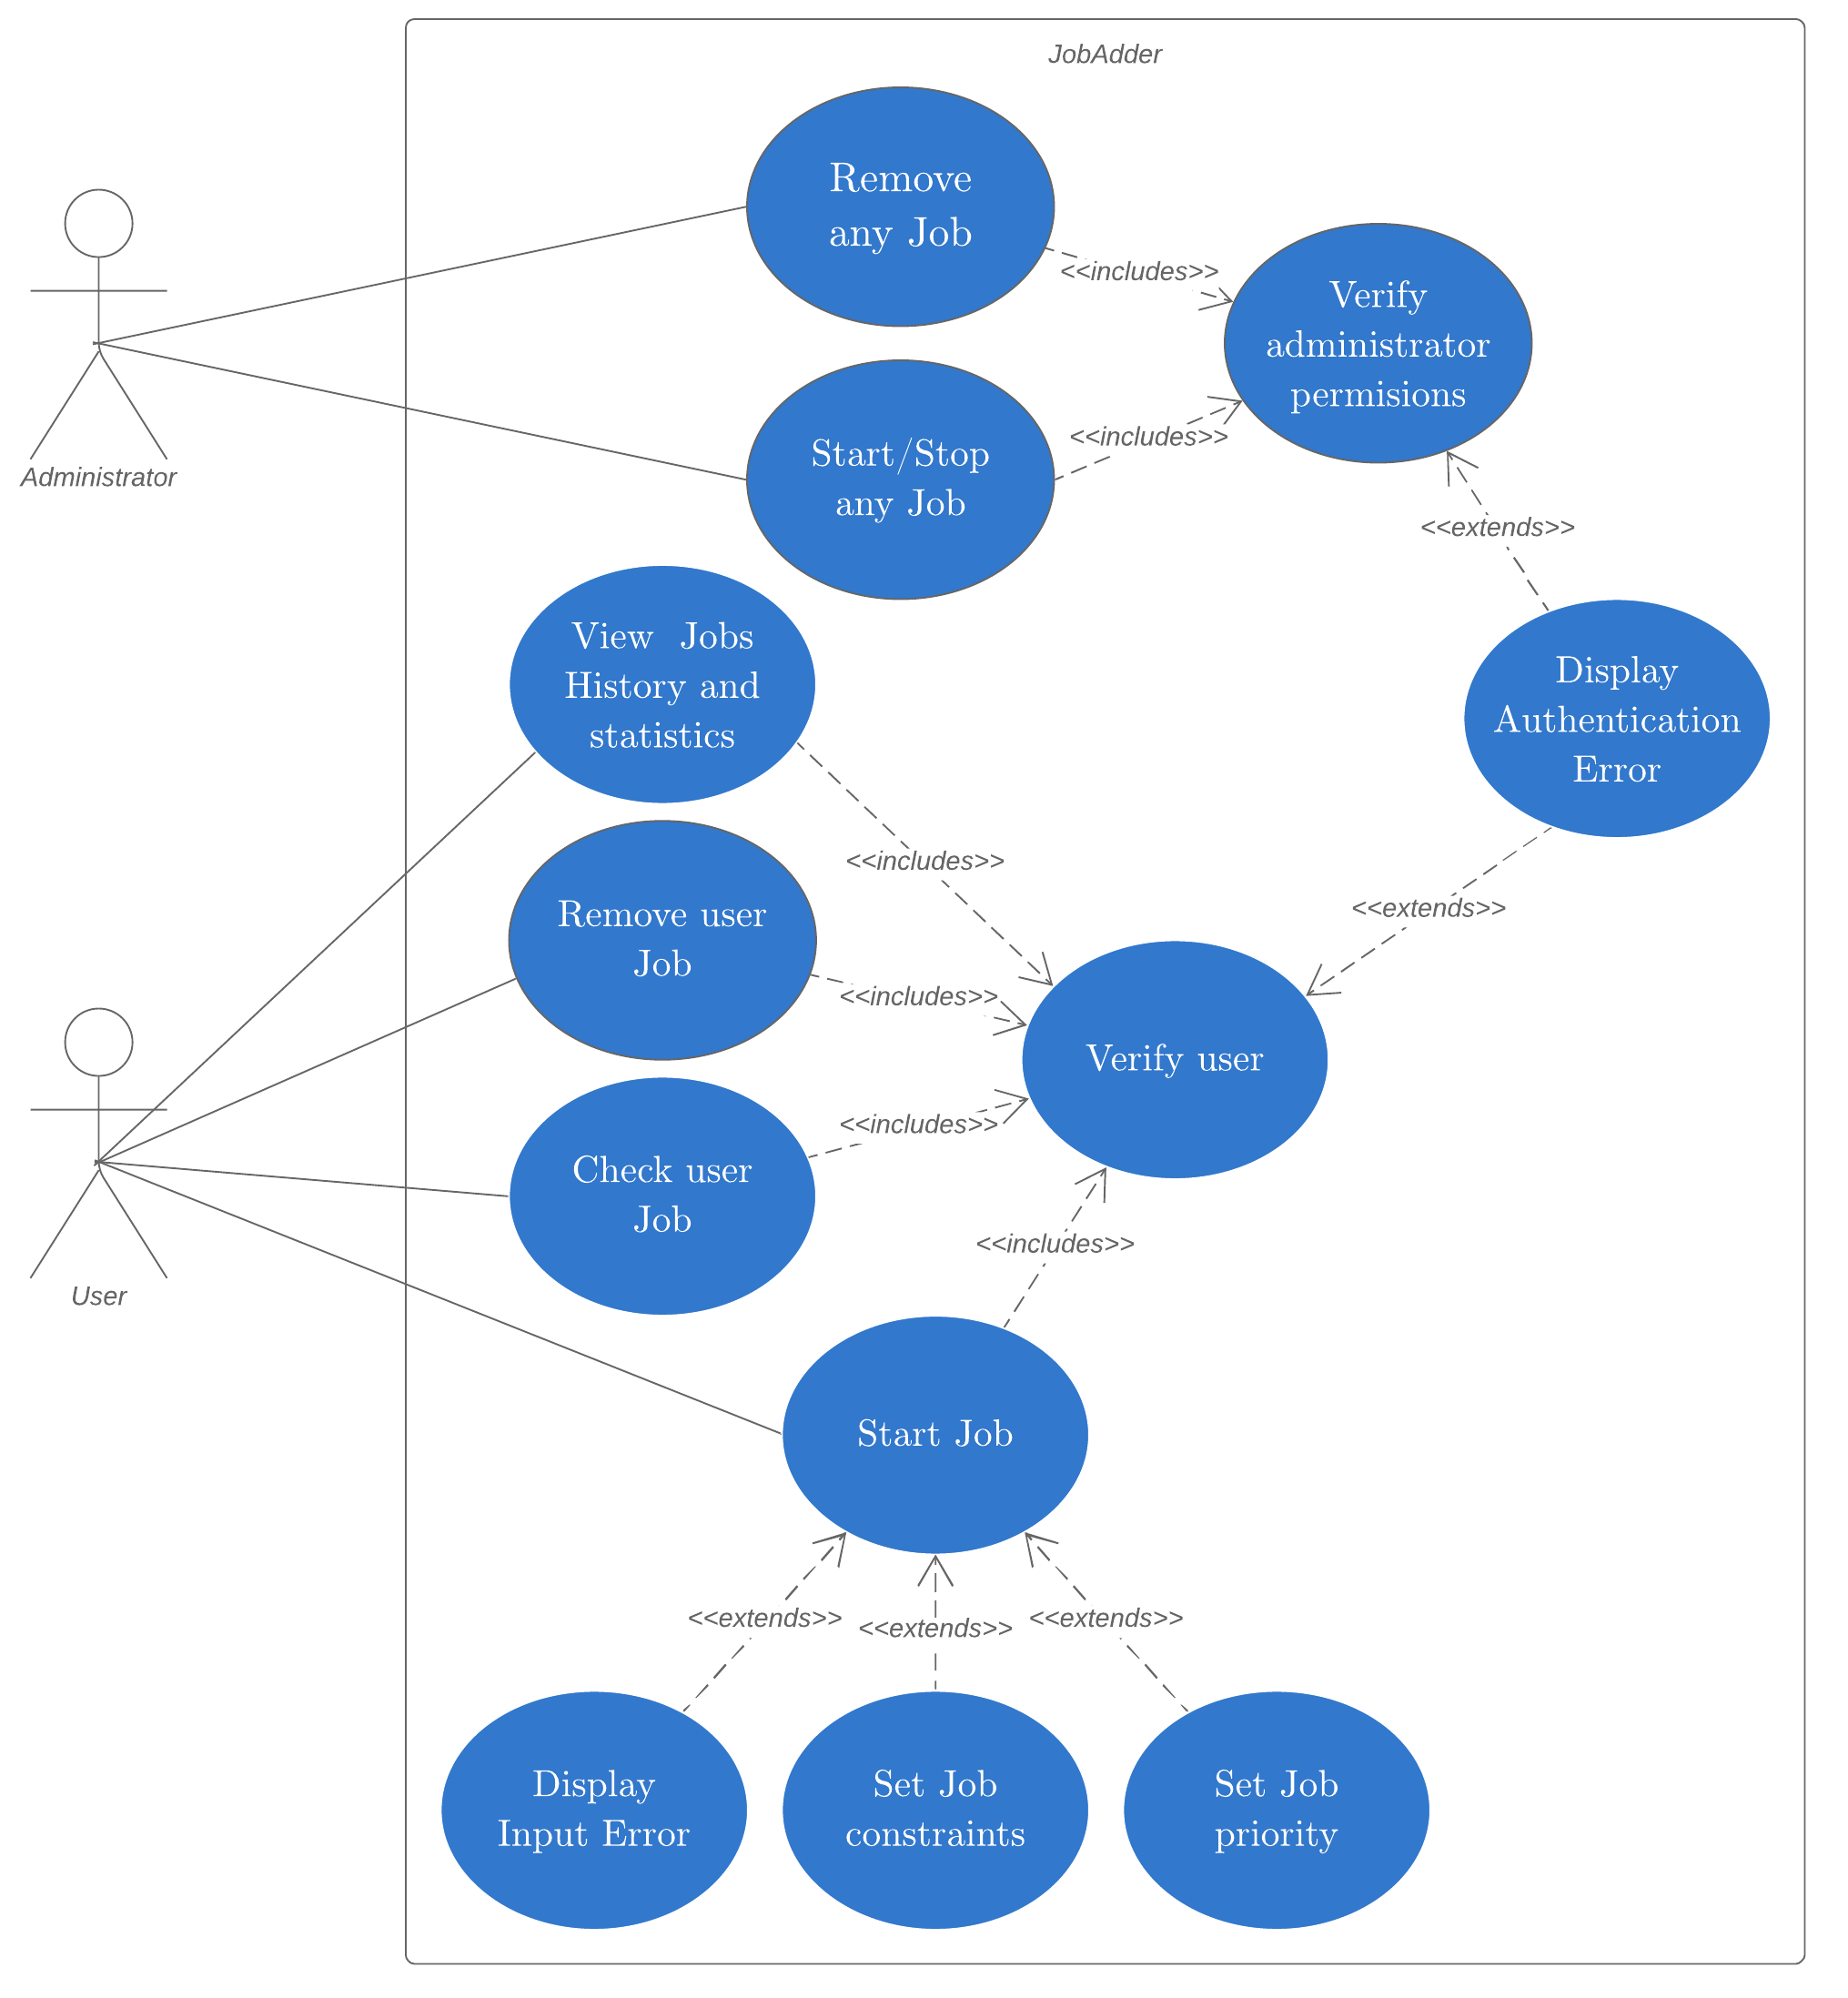
\includegraphics[width=\linewidth]{./system/systemmodel/images/usecasediagram.png}

\subsection{System Model}
\begin{figure}
  \subsubsection{Schedule new Job}
  \centering
  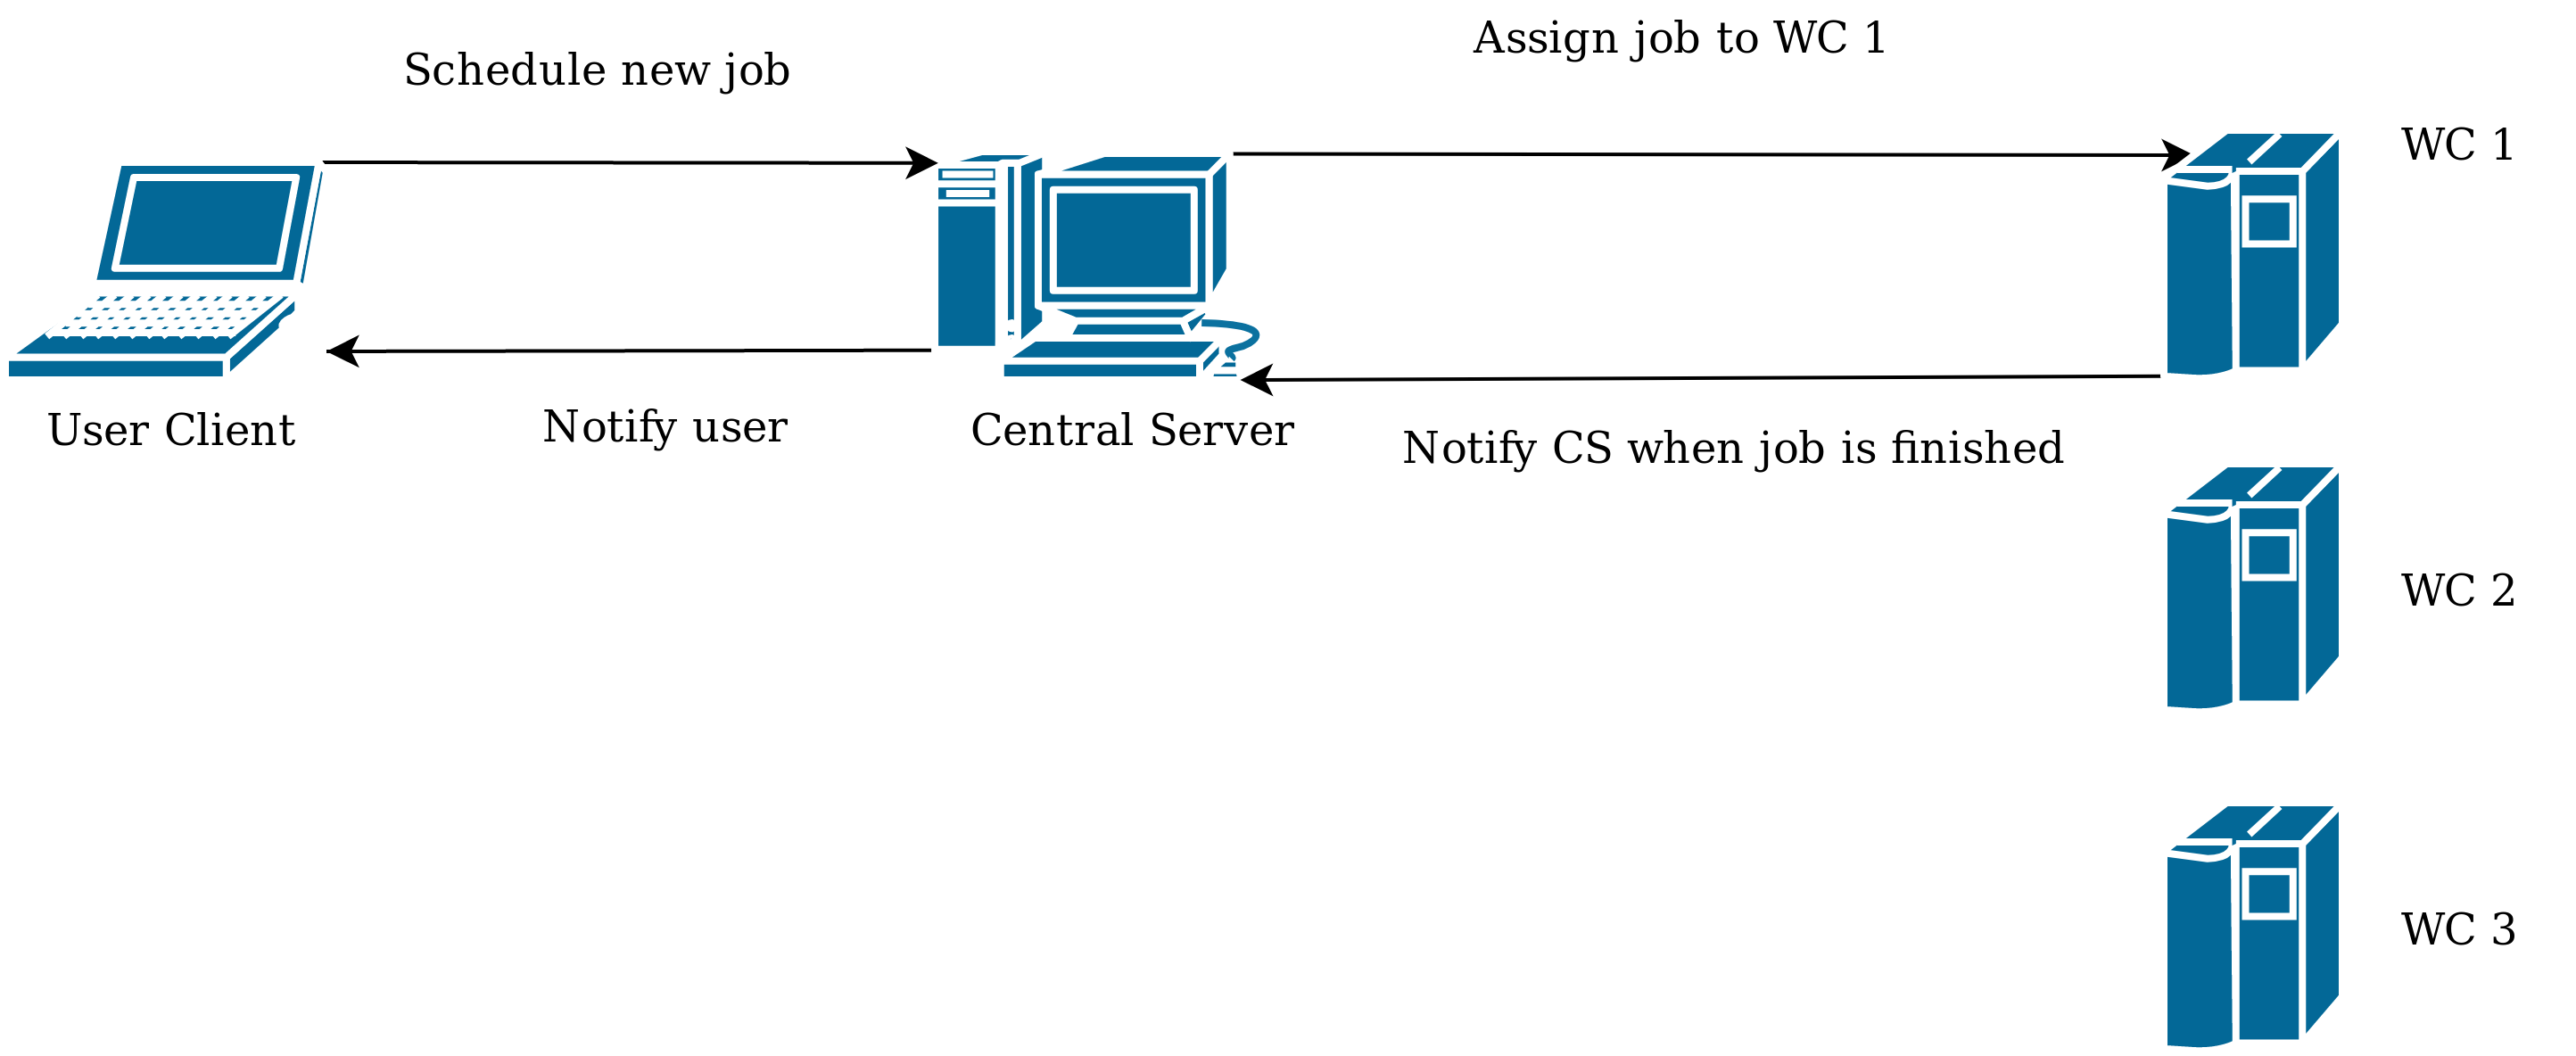
\includegraphics[width=\linewidth]{./system/systemmodel/images/schedulejob.png}
  \label{new-job}
  \caption{This diagram depicts how a user schedules a job, which the CS distributes to WC 1.
  In that case CS knows that there are enough resurces on WC 1 to execute users job.
  At the end the CS notifies the user that the job has finished.}
\end{figure}

\begin{figure}
  \subsubsection{Access a job}
  \centering
  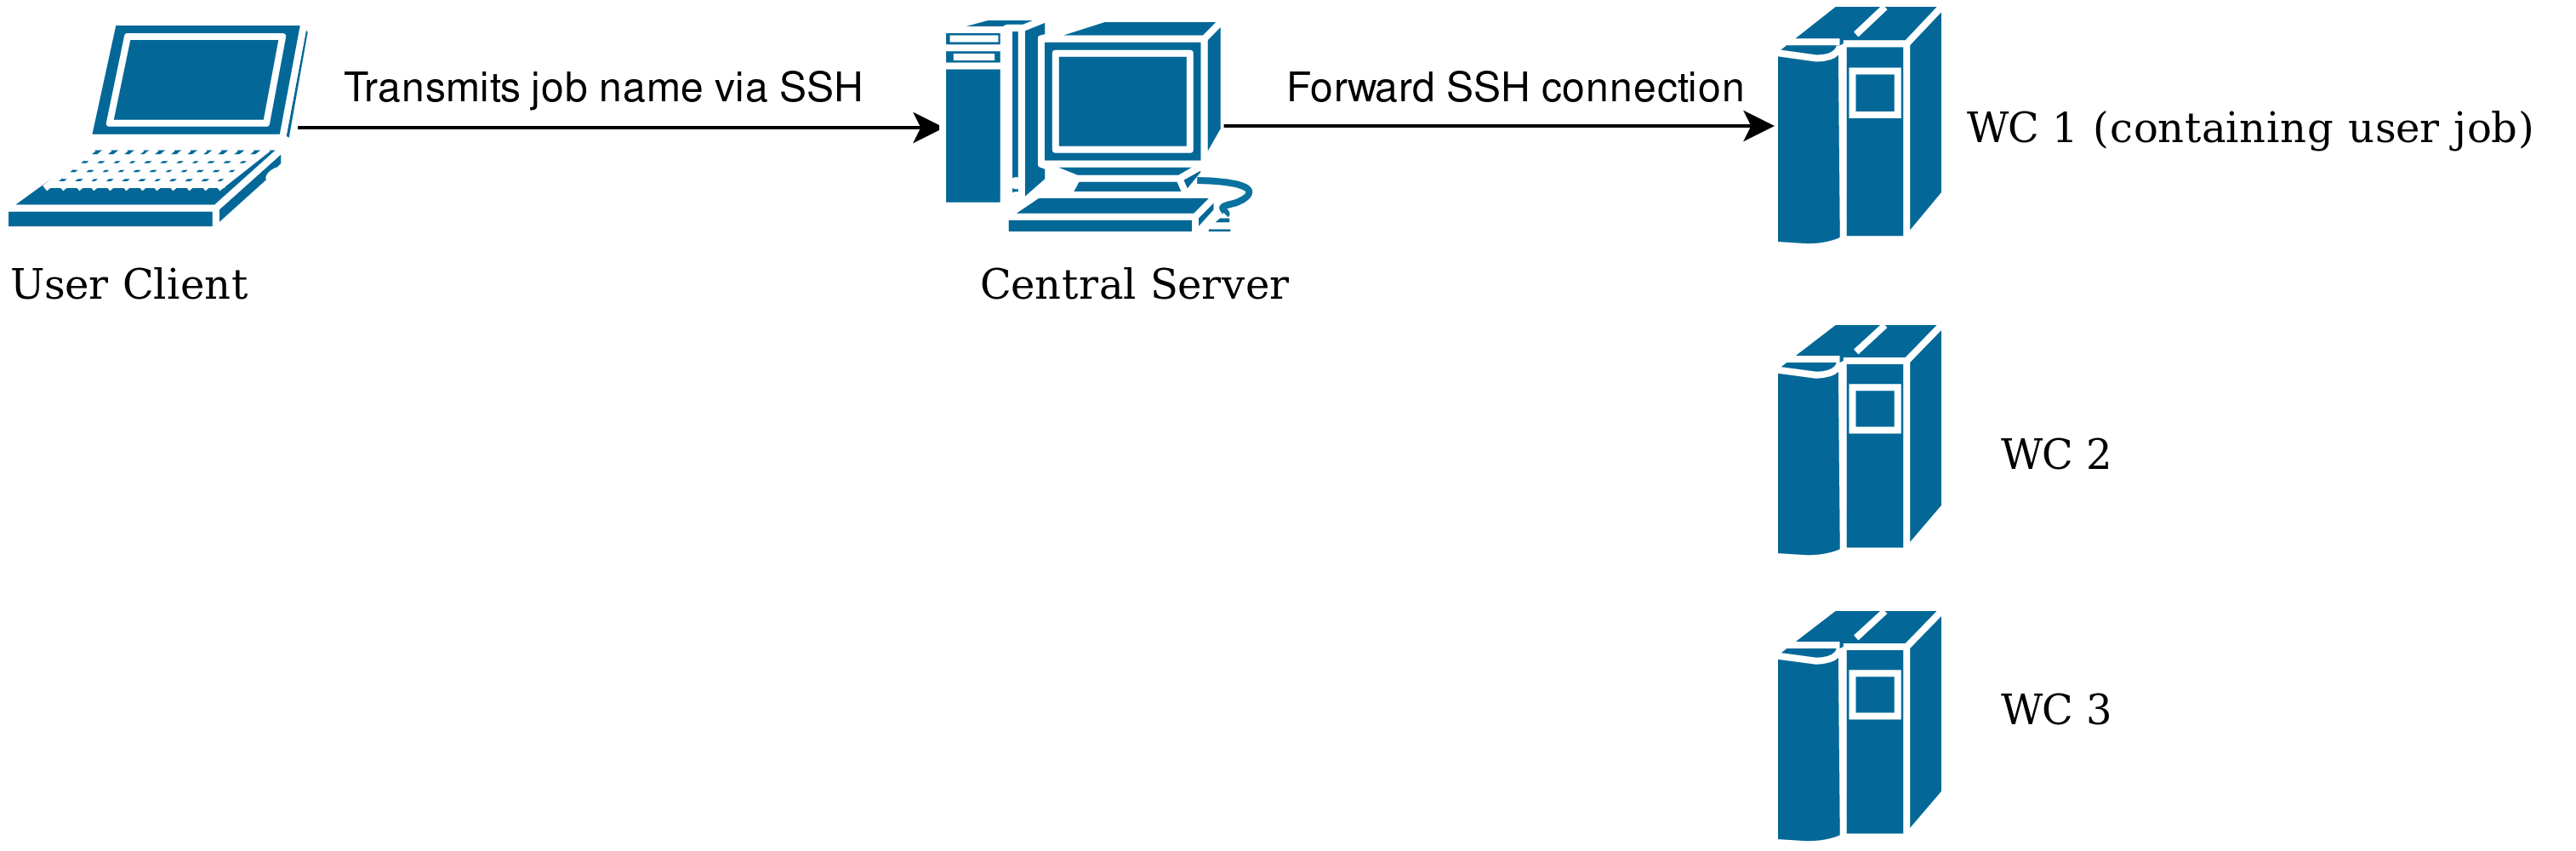
\includegraphics[width=\linewidth]{./system/systemmodel/images/accessjob.png}
  \label{access-job}
  \caption{This diagram depicts how a user accesses his job.
  The user has a job on one of the work machines that he wants to connect to.
  The user does not establish a direct connection with the WC.
  The user establishes an SSH connection to the server.
  This connection authenticates the user.
  It is also used to transmit the name of the job that the user wants to connect to.
  The server looks up which work machine the user's job is located on and forwards the SSH connection to that work machine.
  Finally, the SSH connection to the work machine is forwarded to the container with the user's job.}
\end{figure}

\begin{figure}
  \subsubsection{Get statistics}
  \centering
  
\includegraphics[width=0.5\linewidth]{./system/systemmodel/images/statistics.png}
  \label{statistics}
  \caption{This diagram depicts how a user accesses the statistics saved on the server.}
\end{figure}


\printunsrtglossaries
\end{document}

\chapter{Product Environment}
  \section{User Client}
    \subsection{Hardware Requirements}
      \begin{itemize}
      \item A connection to the central server.
      \item 2 MB of storage space and an additional 100 MB per image.
      \end{itemize}
    \subsection{Software Requirements}
      \begin{itemize}
      \item Python 3.
    \end{itemize}

  \section{Central Server}
    \subsection{Hardware Requirements}
    \begin{itemize}
      \item 500 MB of storage space.
      \item 2 GB of RAM.
      \item One physical CPU core.
    \end{itemize}
    \subsection{Software Requirements}
    \begin{itemize}
      \item Linux Ubuntu 18.04 or newer, or CentOS 7.5 or newer.
      \item MySQL Database Server version 8.0 or newer.
      \item Linux kernel version 3.10 or higher.
      \item CS Docker engine 1.13, EE Deamon 17.03 and higher.
      \item Python 3.
    \end{itemize}

  \section{Working Machine Client}
    \subsection{Hardware Requirements}
      In addition to the hardware required to run a job, our worker client would need the following resources:
    \begin{itemize}
      \item A connection to a LAN.
      \item 4 GB of RAM.
      \item 3 GB of available disk space.
      \item Static IP Address.
    \end{itemize}
    \subsection{Software Requirements}
    \begin{itemize}
      \item Linux kernel version 3.10 or higher.
      \item CS Docker engine 1.13, EE Deamon 17.03 and higher.
      \item Python 3.
    \end{itemize}


\subsection{Scheduling Algorithm}
This section describes how the central server distributes jobs to work machines: the \textit{scheduling algorithm}.
Put briefly, the scheduling algorithm takes a list of jobs and decides which ones to run on the available work machines.
The scheduling algorithm has the following goals:
\begin{itemize}
\item Keep work machines busy: there should be no idle work machines if there are pending jobs.
\item Consider job priorities: jobs with high priorities should be worked on first.
\item Consider time of job submission: jobs that were submitted first should be worked on first (if priorities are equal).
\end{itemize}
The scheduling algorithm operates under the following conditions:
\begin{itemize}
\item Jobs arrive at unforeseen times.
\item Time required to complete jobs is unknown.
\item Jobs cannot be transferred from one work machine to another.
\item Jobs cannot be canceled and restarted.
\item Job preemption is limited: if a job is paused it has to be kept in memory.
Note that memory includes swap files.
\item Some jobs cannot be paused due to software licensing restrictions.
\end{itemize}
The scheduling algorithm takes the following parameters as input:
\begin{itemize}
\item List of pending jobs.
\item List of running/paused jobs per work machine.
\item Amount of work machine specific resources: CPU threads, memory, etc.
These resources can typically be freed by pausing jobs.
\item Amount of work machine unspecific resources: software licenses.
Whether these resources can be freed by pausing jobs depends on the software.
\item Size of work machine swap files.
This resource is used exclusively for holding paused jobs.
It has no influence on running jobs.
\end{itemize}
The scheduling algorithm reevaluates which jobs to run every time a job finishes running or when a new job request arrives.
The scheduling algorithm assigns jobs to work machines as follows:
\begin{enumerate}
\item If there are pending urgent jobs:
Assign oldest urgent jobs to work machines until urgent jobs or resources run out.
Non-urgent running jobs will be paused if possible and necessary to run more urgent jobs.
\item If there are paused high-priority jobs:
Assign oldest paused high-priority jobs to work machines until paused high-priority jobs or resources run out.
Running jobs with equal or lower priority will be paused if possible and necessary to run more old paused high-priority jobs.
\item Repeat 2. for paused medium-priority jobs.
\item Repeat 2. for paused low-priority jobs.
\item If there are pending high-priority jobs:
Assign oldest paused high-priority jobs to work machines until paused high-priority jobs or resources run out.
Running jobs with equal or lower priority will be paused if possible and necessary to run the oldest available high-priority job.
\item Repeat 5. for pending medium-priority jobs.
\item Repeat 5. for pending low-priority jobs.
\end{enumerate}
\newcommand{\jacommand}[3]{
\textsc{\LARGE{\textbf{#1}}}
\begin{itemize}
\item \textbf{Options:} #2
\item \textbf{Effect:} #3
\end{itemize}
}
\newcommand{\jaoptionheader}{\textsc{\textbf{Option descriptions:}}\newline\newline}
\newcommand{\jaoption}[3]{
\textbf{#1}
\begin{itemize}
\item \textbf{Short form:} #2
\item \textbf{Effect:} #3
\end{itemize}
}
\subsection{Command Line Interface}
All components of JobAdder are accessible through a command line interface (CLI).
The command line interface on a machine with JobAdder installed has the following structure:
\begin{equation}
\text{<component name> <command> <options> <targets>},
\end{equation}
where the \textit{component name} can be any one of the following:
\begin{itemize}
\item \textbf{jobadder} to access the \textit{user client}.
\item \textbf{jobcenter} to access the \textit{server}.
\item \textbf{jobworker} to access the \textit{worker client}.
\end{itemize}
Commands, options, and valid targets are and options are specified in the following sections.

Options can be added in the following ways:
\begin{itemize}
\item By supplying their names like "-{}-option\_x -{}-option\_y=2 -{}-option\_z".
\item By supplying their abbreviations like "-x -y 2 -z".
\item By supplying their abbreviations like "-xz -y 2".
\end{itemize}

The available \textit{commands} are generally specific to the used component.
Likewise, the available \textit{options} and \textit{targets} are generally specific to the commands of a used component.
However, some commands and options are shared between components or commands.

The JobAdder CLI only uses lower-case letters.
JobAdder CLI options override the values of configuration files.
If no command is given, the general help text for the given component is printed out.
\subsubsection{Shared Options}
\jaoption{config}{c}{Overrides the global configuration file with the given configuration file.}
\jaoption{detach}{d}{Detaches the execution of the given command from the command line.}
\jaoption{help}{h}{
Prints out a list of the available commands. 
When used in conjunction with a command:
prints out more detailed information on the given command and a list of the available options.}
\jaoption{verbose}{v}{
Determines the amount of information printed out.
If set to 2, detailed information is printed out.
If set to 1, only high-level information is printed out (default).
If set to 0, no information is printed out.}
\subsubsection{User Client}
\jacommand{add}
{gpu, mount, name, priority, server, ram, threads}
{Sends one or more job requests to the server.
If targets are Docker containers the job consists of simply running the container.
If targets are configuration files with a specified terminal command the job consists of running the specified terminal command.
Otherwise targets are interpreted as terminal commands}
\jaoptionheader
\jaoption{gpu}{g}{
If set to true, informs the server that the job requires a gpu.
If set to a string that can be interpreted as VRAM amount, informs the server that a GPU with this amount of VRAM is required for the job.
If set to a specific GPU model, informs the server that the job must be run on a machine with that GPU built in.
}
\jaoption{mount}{m}
{Directories that need to be mounted onto the Docker container that the job is running in.}
\jaoption{name}{n}
{Human-readable name of the job.
Defaults to user's name + job index}
\jaoption{priority}{p}
{Sets the priority of the job: urgent, high, medium, or low.
Defaults to medium.}
\jaoption{server}{s}
{Server to send the job request to.
Defaults to localhost.}
\jaoption{ram}{r}
{If set to a string that can be interpreted as RAM amount, informs the server that this amount of RAM is required for the job.}
\jaoption{threads}{t}
{If set to an integer, informs the server that this number of threads is required for the job.}
\jacommand{query}{user}
{Prints out information on running/queued/past jobs (specified by target).
In addition to the one below, options from add command can be used as constraints.}
\jaoptionheader
\jaoption{after}{a}{Only return jobs added after the given point in time.}
\jaoption{before}{b}{Only return jobs added before the given point in time.}
\jaoption{user}{u}{Filter query by user that added the job.}
\jacommand{stop}{None}{Stops the job with the specified name.}
\subsubsection{Server}
\jacommand{start}{None}{Starts an instance of the JobAdder server.}
\jacommand{stop}{None}{Stops instances of the JobAdder server.}
\subsubsection{Worker Client}
\jacommand{start}{server}{Starts an instance of the JobAdder worker client.}
\jaoptionheader
\jaoption{server}{s}
{Server to receive jobs from.
Defaults to localhost.}
\jacommand{stop}{None}{Stops instances of the JobAdder worker client.}

\documentclass[a4paper,10pt]{scrreprt}
\usepackage[T1]{fontenc}
\usepackage[utf8]{inputenc}
\usepackage[nonumberlist,nopostdot]{glossaries-extra}     % provides glossary commands
\usepackage{graphicx}       % provides commands for including figures
\usepackage{amsmath}
\usepackage{float}
\usepackage{hyperref}

% Glossary needs to be before \begin{document}
\newglossaryentry{ID}
{
  name=ID,
  plural=IDs,
  description={
    An ID is a string of digits, english letters (both lower- and uppercase) and slashes '-'.
  }
}
\newglossaryentry{job status}
{
  name=job status,
  plural=job status,
  description={
    The status of a job can be:
    \begin{itemize}
      \item Queued - the job is waiting for a suitable work machine to become available.
      \item Running - the job is running on some work machine.
      \item Paused - the job has been running, but has been paused to allow for execution of other jobs.
      \item Done - the job has finished running.
      \item Killed - the job was forcefully stopped.
      \item Crashed - the work machine the job was running on shut down unexpectedly.
    \end{itemize}
  }
}
\newglossaryentry{job priority}
{
  name=job priority,
  plural=job priorities,
  description={
    The priority of a job can be one of the following (in ascending order):
    \begin{itemize}
      \item Low
      \item Medium
      \item High
      \item Urgent
    \end{itemize}
  }
}
\newglossaryentry{job}
{
  name=job,
  plural=jobs,
  description={
      A job in the context of JobAdder consists of the following:
      \begin{itemize}
        \item A unique job \gls{ID}.
        \item A program to be executed.
        \item A unix user who owns the job.
        \item \Gls{job priority}.
        \item Number of CPU threads needed for the execution of the program, an integer.
        \item Amount of RAM in megabytes needed for the execution of the program, an integer.
        \item Paths in the network storage needed for the application.
        \item One of:
        \begin{itemize}
          \item A Dockerfile providing instructions to build program environment.
          \item The name of predefined container environment, for ex. a base image from Docker Hub.
        \end{itemize}
     \end{itemize}
  }
}
\newglossaryentry{timestamp}
{
  name=timestamp,
  plural=timestamps,
  description={
    A timestamp is a combination of the date and time of a particular point in time.
    It has the following format: "YYYY-DD-MM HH:MM:SS".
  }
}
\newglossaryentry{administrator}
{
  name=administrator,
  plural=administrators,
  description={
    An administrator is a user who can terminate queued and running jobs from all users.
  }
}
\newglossaryentry{UID}
{
  name=UID,
  plural=UIDs,
  description={
    A UID (user identifier) is a number assigned by Linux to each user on the system.
  }
}
\newglossaryentry{GID}
{
  name=GID,
  plural=GIDs,
  description={
    A GID (group identifier) is a number assigned by Linux to each group on the system.
  }
}
\newglossaryentry{Dockerfile}
{
  name=Dockerfile,
  plural=Dockerfiles,
  description={
     A Dockerfile is a text document that contains all the commands a user could call on the
     command line to assemble an image.
  }
}


%opening
\title{JobAdder: Requirements}
\author{Johannes Gäßler \and  Ilia Bozhinov \and Nikola Tzotchev \and Malik Bouguila \and Jamil Bagga}

\begin{document}

\maketitle
\tableofcontents
\newpage

\section{Introduction}
The JobAdder project enables users to remotely execute resource-intensive tasks on a dedicated cluster of work machines.
Tasks are being distributed to work machines automatically.\newline
The distribution reduces task execution times and peak system loads by better utilizing the available hardware.
In addition, JobAdder provides tools to inspect the state of the whole system and display statistics about user activity.
\section{Purpose}
  \subsection{Product Goal}
    JobAdder aims to facilitate and accelerate the execution of computationally
    expensive jobs in a cluster of work machines.

    Currently, users need to access every single work machine manually in order to
    distribute their jobs over them. Even more problems arise when a group of users
    is involved. In that case, users have to look for the work machine with the
    least amount of work and add their job to it.
   
    JobAdder addresses and solves these problems. With JobAdder, users are able to
    send their jobs to a central server in order to evenly distribute them over
    suitable work machines without having to look for them manually. So if there is
    enough workload (which is usually the case), no machine remains idle unless it
    is forced to.

    Jobadder also aims to make task scheduling more user-friendly. A user does not
    have to keep checking the state of their job, they will be notified once the job
    is done. Nor does a user have to wait for an idle machine in order to queue a
    job, the central server saves them up and runs them once it is possible. There
    is also more insight into the whole system by providing statistics about user
    activity, currently running jobs, past jobs and queued jobs.
   
    Users can set priorities for their jobs so that jobs with high priority will be
    executed before jobs with low priority. Urgent jobs are immediately executed by
    pausing jobs with the lowest priority, so a user is not required to pause or
    cancel low-priority jobs manually. The scheduling algorithm also guarantees that
    every job is eventually run by automatically increasing it's priority over time.

  \subsection{Target Audience}
    The target audience mostly consists of groups of users with access to several
    work machines. This includes, companies, academic institutions and computing
    centers. These users usually need remote machines to run their jobs due to high
    hardware requirements.
   
    JobAdder helps them use their hardware more efficiently by adding an abstraction
    layer between the user and the work machines that are running the user's jobs.
\documentclass[a4paper,10pt]{scrreprt}
\usepackage[T1]{fontenc}
\usepackage[utf8]{inputenc}
\usepackage[nonumberlist,nopostdot]{glossaries-extra}     % provides glossary commands
\usepackage{graphicx}       % provides commands for including figures
\usepackage{amsmath}
\usepackage{float}
\usepackage{hyperref}

% Glossary needs to be before \begin{document}
\input{customer/glossary}

%opening
\title{JobAdder: Requirements}
\author{Johannes Gäßler \and  Ilia Bozhinov \and Nikola Tzotchev \and Malik Bouguila \and Jamil Bagga}

\begin{document}

\maketitle
\tableofcontents
\newpage

\input{customer/introduction}
\input{customer/goals}
\input{customer/main}
\input{customer/product-environment}
\input{customer/scheduling-algorithm}
\input{customer/cli}
\input{system/main}

\newpage
\input{system/systemmodel/use-case-diagram}
\input{system/systemmodel/system-model.tex}

\printunsrtglossaries
\end{document}

\chapter{Product Environment}
  \section{User Client}
    \subsection{Hardware Requirements}
      \begin{itemize}
      \item A connection to the central server.
      \item 2 MB of storage space and an additional 100 MB per image.
      \end{itemize}
    \subsection{Software Requirements}
      \begin{itemize}
      \item Python 3.
    \end{itemize}

  \section{Central Server}
    \subsection{Hardware Requirements}
    \begin{itemize}
      \item 500 MB of storage space.
      \item 2 GB of RAM.
      \item One physical CPU core.
    \end{itemize}
    \subsection{Software Requirements}
    \begin{itemize}
      \item Linux Ubuntu 18.04 or newer, or CentOS 7.5 or newer.
      \item MySQL Database Server version 8.0 or newer.
      \item Linux kernel version 3.10 or higher.
      \item CS Docker engine 1.13, EE Deamon 17.03 and higher.
      \item Python 3.
    \end{itemize}

  \section{Working Machine Client}
    \subsection{Hardware Requirements}
      In addition to the hardware required to run a job, our worker client would need the following resources:
    \begin{itemize}
      \item A connection to a LAN.
      \item 4 GB of RAM.
      \item 3 GB of available disk space.
      \item Static IP Address.
    \end{itemize}
    \subsection{Software Requirements}
    \begin{itemize}
      \item Linux kernel version 3.10 or higher.
      \item CS Docker engine 1.13, EE Deamon 17.03 and higher.
      \item Python 3.
    \end{itemize}


\subsection{Scheduling Algorithm}
This section describes how the central server distributes jobs to work machines: the \textit{scheduling algorithm}.
Put briefly, the scheduling algorithm takes a list of jobs and decides which ones to run on the available work machines.
The scheduling algorithm has the following goals:
\begin{itemize}
\item Keep work machines busy: there should be no idle work machines if there are pending jobs.
\item Consider job priorities: jobs with high priorities should be worked on first.
\item Consider time of job submission: jobs that were submitted first should be worked on first (if priorities are equal).
\end{itemize}
The scheduling algorithm operates under the following conditions:
\begin{itemize}
\item Jobs arrive at unforeseen times.
\item Time required to complete jobs is unknown.
\item Jobs cannot be transferred from one work machine to another.
\item Jobs cannot be canceled and restarted.
\item Job preemption is limited: if a job is paused it has to be kept in memory.
Note that memory includes swap files.
\item Some jobs cannot be paused due to software licensing restrictions.
\end{itemize}
The scheduling algorithm takes the following parameters as input:
\begin{itemize}
\item List of pending jobs.
\item List of running/paused jobs per work machine.
\item Amount of work machine specific resources: CPU threads, memory, etc.
These resources can typically be freed by pausing jobs.
\item Amount of work machine unspecific resources: software licenses.
Whether these resources can be freed by pausing jobs depends on the software.
\item Size of work machine swap files.
This resource is used exclusively for holding paused jobs.
It has no influence on running jobs.
\end{itemize}
The scheduling algorithm reevaluates which jobs to run every time a job finishes running or when a new job request arrives.
The scheduling algorithm assigns jobs to work machines as follows:
\begin{enumerate}
\item If there are pending urgent jobs:
Assign oldest urgent jobs to work machines until urgent jobs or resources run out.
Non-urgent running jobs will be paused if possible and necessary to run more urgent jobs.
\item If there are paused high-priority jobs:
Assign oldest paused high-priority jobs to work machines until paused high-priority jobs or resources run out.
Running jobs with equal or lower priority will be paused if possible and necessary to run more old paused high-priority jobs.
\item Repeat 2. for paused medium-priority jobs.
\item Repeat 2. for paused low-priority jobs.
\item If there are pending high-priority jobs:
Assign oldest paused high-priority jobs to work machines until paused high-priority jobs or resources run out.
Running jobs with equal or lower priority will be paused if possible and necessary to run the oldest available high-priority job.
\item Repeat 5. for pending medium-priority jobs.
\item Repeat 5. for pending low-priority jobs.
\end{enumerate}
\newcommand{\jacommand}[3]{
\textsc{\LARGE{\textbf{#1}}}
\begin{itemize}
\item \textbf{Options:} #2
\item \textbf{Effect:} #3
\end{itemize}
}
\newcommand{\jaoptionheader}{\textsc{\textbf{Option descriptions:}}\newline\newline}
\newcommand{\jaoption}[3]{
\textbf{#1}
\begin{itemize}
\item \textbf{Short form:} #2
\item \textbf{Effect:} #3
\end{itemize}
}
\subsection{Command Line Interface}
All components of JobAdder are accessible through a command line interface (CLI).
The command line interface on a machine with JobAdder installed has the following structure:
\begin{equation}
\text{<component name> <command> <options> <targets>},
\end{equation}
where the \textit{component name} can be any one of the following:
\begin{itemize}
\item \textbf{jobadder} to access the \textit{user client}.
\item \textbf{jobcenter} to access the \textit{server}.
\item \textbf{jobworker} to access the \textit{worker client}.
\end{itemize}
Commands, options, and valid targets are and options are specified in the following sections.

Options can be added in the following ways:
\begin{itemize}
\item By supplying their names like "-{}-option\_x -{}-option\_y=2 -{}-option\_z".
\item By supplying their abbreviations like "-x -y 2 -z".
\item By supplying their abbreviations like "-xz -y 2".
\end{itemize}

The available \textit{commands} are generally specific to the used component.
Likewise, the available \textit{options} and \textit{targets} are generally specific to the commands of a used component.
However, some commands and options are shared between components or commands.

The JobAdder CLI only uses lower-case letters.
JobAdder CLI options override the values of configuration files.
If no command is given, the general help text for the given component is printed out.
\subsubsection{Shared Options}
\jaoption{config}{c}{Overrides the global configuration file with the given configuration file.}
\jaoption{detach}{d}{Detaches the execution of the given command from the command line.}
\jaoption{help}{h}{
Prints out a list of the available commands. 
When used in conjunction with a command:
prints out more detailed information on the given command and a list of the available options.}
\jaoption{verbose}{v}{
Determines the amount of information printed out.
If set to 2, detailed information is printed out.
If set to 1, only high-level information is printed out (default).
If set to 0, no information is printed out.}
\subsubsection{User Client}
\jacommand{add}
{gpu, mount, name, priority, server, ram, threads}
{Sends one or more job requests to the server.
If targets are Docker containers the job consists of simply running the container.
If targets are configuration files with a specified terminal command the job consists of running the specified terminal command.
Otherwise targets are interpreted as terminal commands}
\jaoptionheader
\jaoption{gpu}{g}{
If set to true, informs the server that the job requires a gpu.
If set to a string that can be interpreted as VRAM amount, informs the server that a GPU with this amount of VRAM is required for the job.
If set to a specific GPU model, informs the server that the job must be run on a machine with that GPU built in.
}
\jaoption{mount}{m}
{Directories that need to be mounted onto the Docker container that the job is running in.}
\jaoption{name}{n}
{Human-readable name of the job.
Defaults to user's name + job index}
\jaoption{priority}{p}
{Sets the priority of the job: urgent, high, medium, or low.
Defaults to medium.}
\jaoption{server}{s}
{Server to send the job request to.
Defaults to localhost.}
\jaoption{ram}{r}
{If set to a string that can be interpreted as RAM amount, informs the server that this amount of RAM is required for the job.}
\jaoption{threads}{t}
{If set to an integer, informs the server that this number of threads is required for the job.}
\jacommand{query}{user}
{Prints out information on running/queued/past jobs (specified by target).
In addition to the one below, options from add command can be used as constraints.}
\jaoptionheader
\jaoption{after}{a}{Only return jobs added after the given point in time.}
\jaoption{before}{b}{Only return jobs added before the given point in time.}
\jaoption{user}{u}{Filter query by user that added the job.}
\jacommand{stop}{None}{Stops the job with the specified name.}
\subsubsection{Server}
\jacommand{start}{None}{Starts an instance of the JobAdder server.}
\jacommand{stop}{None}{Stops instances of the JobAdder server.}
\subsubsection{Worker Client}
\jacommand{start}{server}{Starts an instance of the JobAdder worker client.}
\jaoptionheader
\jaoption{server}{s}
{Server to receive jobs from.
Defaults to localhost.}
\jacommand{stop}{None}{Stops instances of the JobAdder worker client.}

\documentclass[a4paper,10pt]{scrreprt}
\usepackage[T1]{fontenc}
\usepackage[utf8]{inputenc}
\usepackage[nonumberlist,nopostdot]{glossaries-extra}     % provides glossary commands
\usepackage{graphicx}       % provides commands for including figures
\usepackage{amsmath}
\usepackage{float}
\usepackage{hyperref}

% Glossary needs to be before \begin{document}
\input{customer/glossary}

%opening
\title{JobAdder: Requirements}
\author{Johannes Gäßler \and  Ilia Bozhinov \and Nikola Tzotchev \and Malik Bouguila \and Jamil Bagga}

\begin{document}

\maketitle
\tableofcontents
\newpage

\input{customer/introduction}
\input{customer/goals}
\input{customer/main}
\input{customer/product-environment}
\input{customer/scheduling-algorithm}
\input{customer/cli}
\input{system/main}

\newpage
\input{system/systemmodel/use-case-diagram}
\input{system/systemmodel/system-model.tex}

\printunsrtglossaries
\end{document}


\newpage
\subsection{Use Case Diagram}
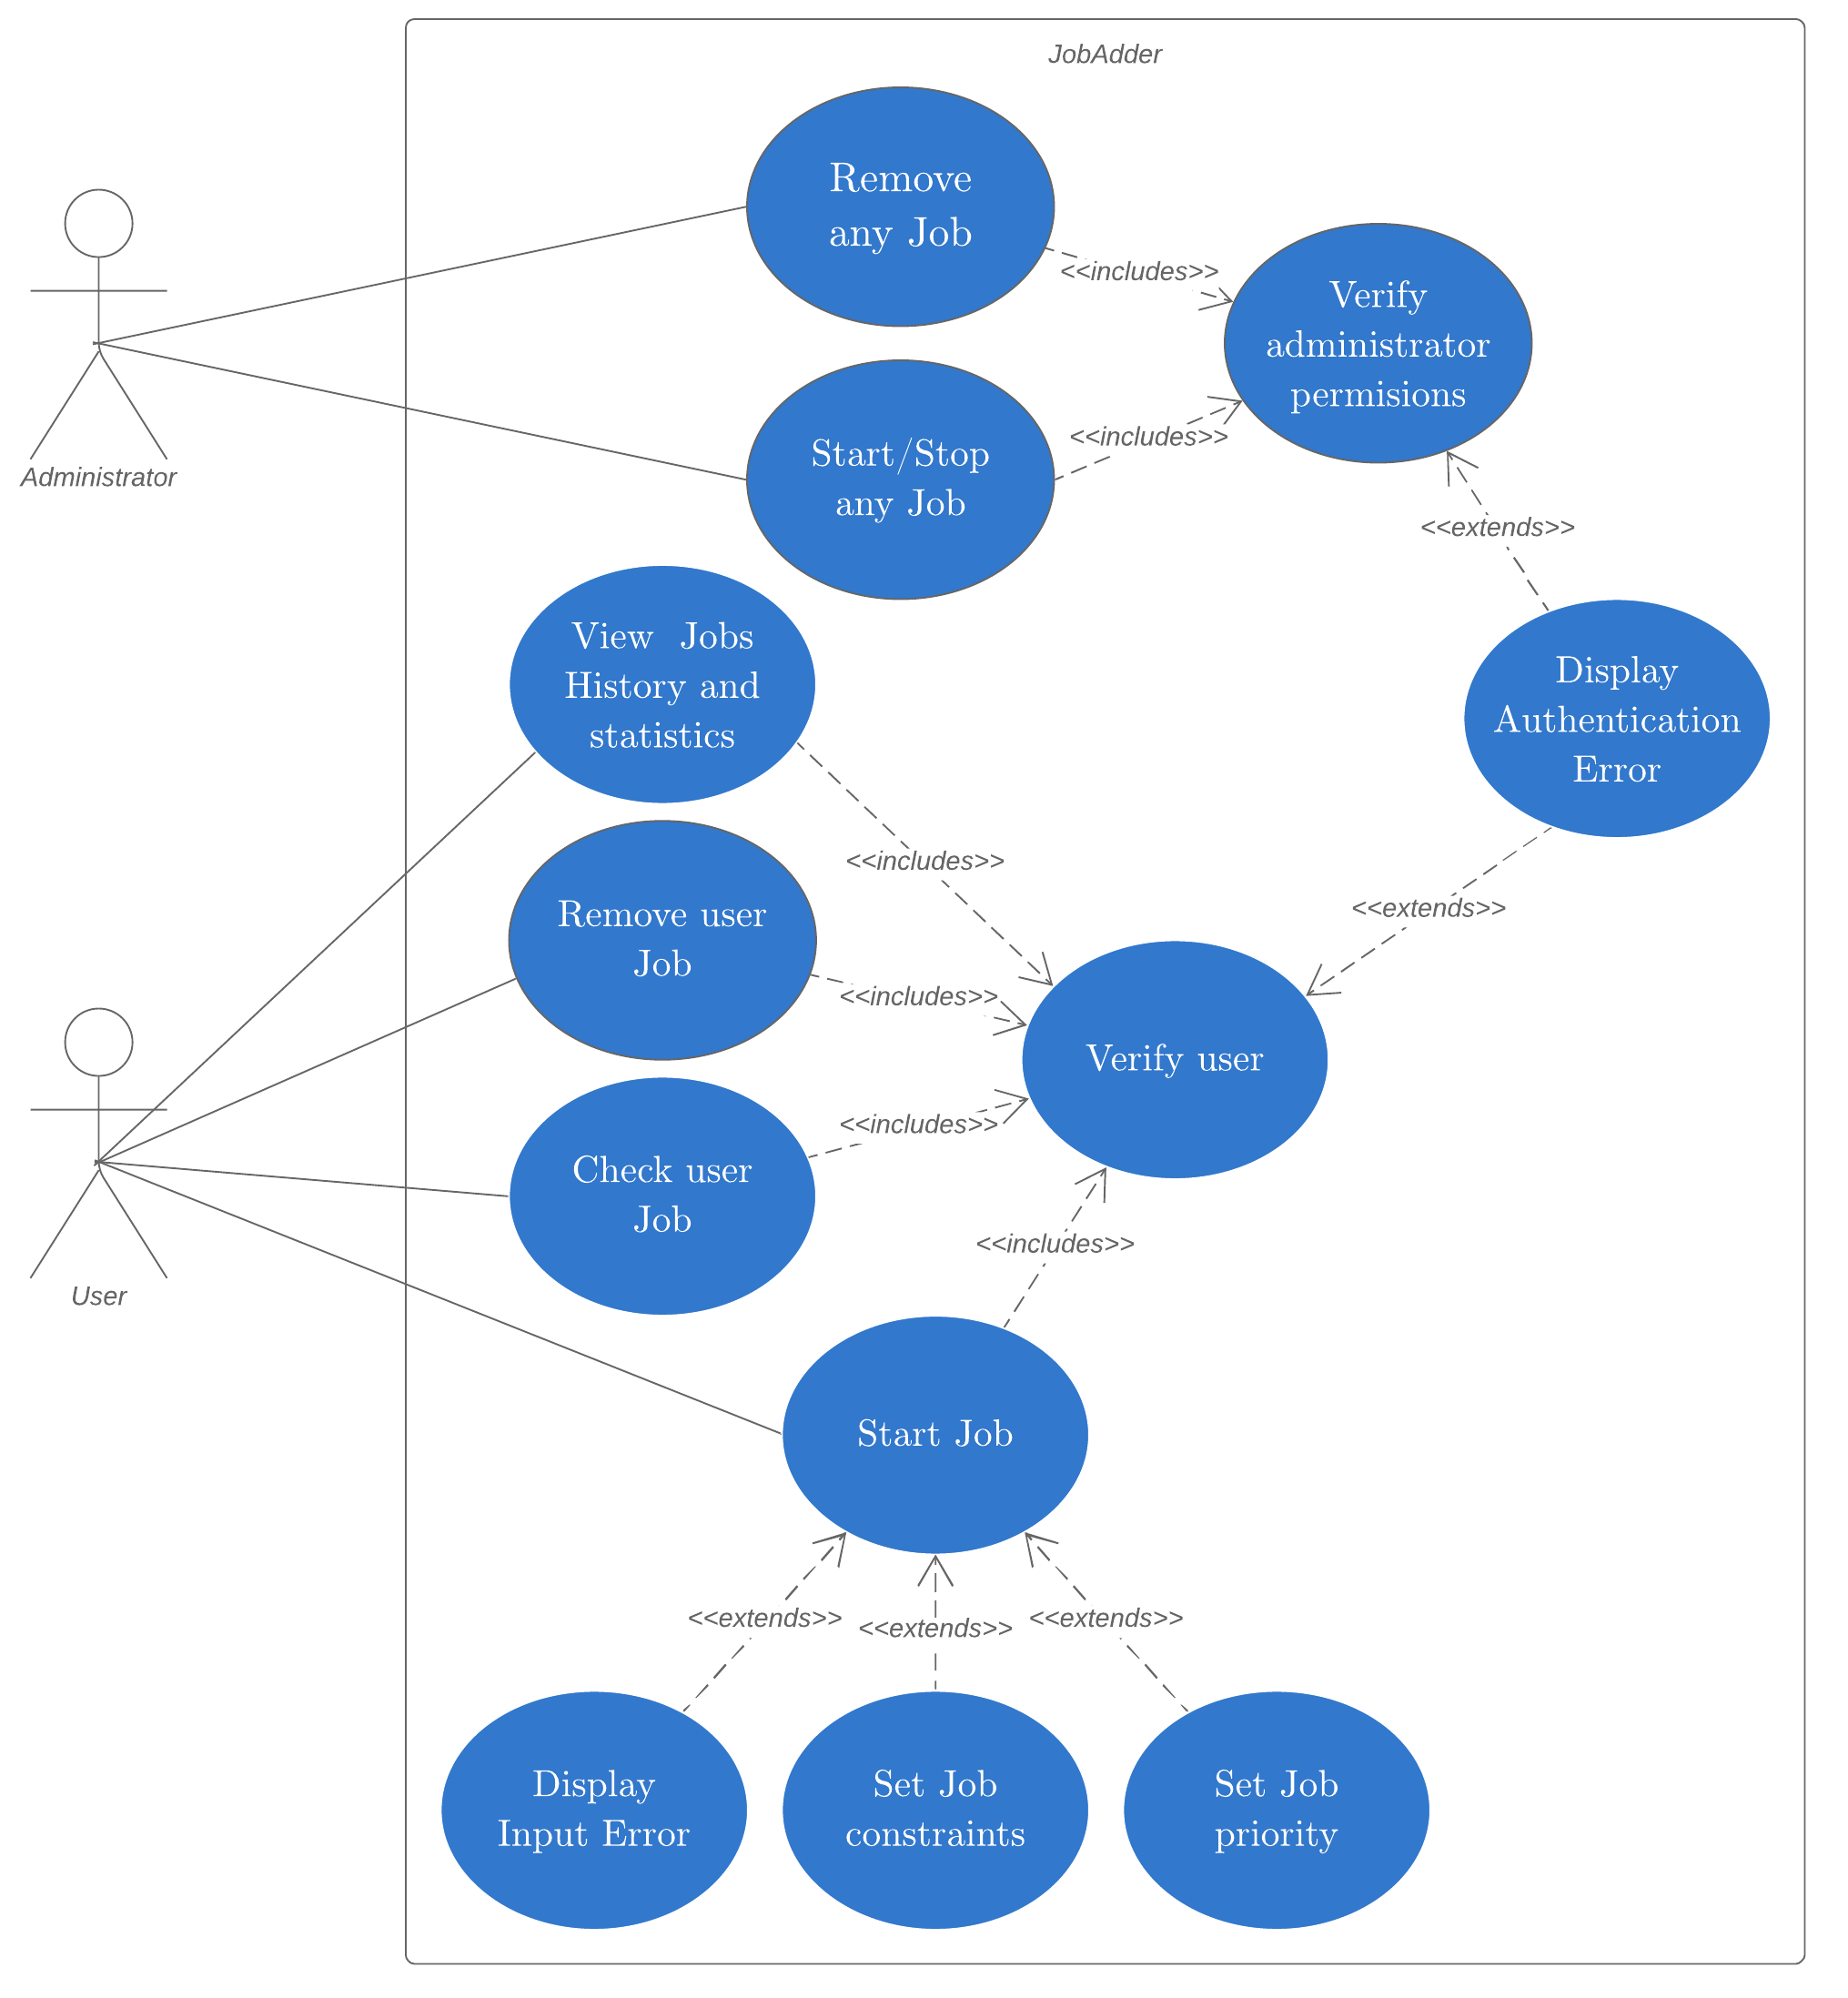
\includegraphics[width=\linewidth]{./system/systemmodel/images/usecasediagram.png}

\subsection{System Model}
\begin{figure}
  \subsubsection{Schedule new Job}
  \centering
  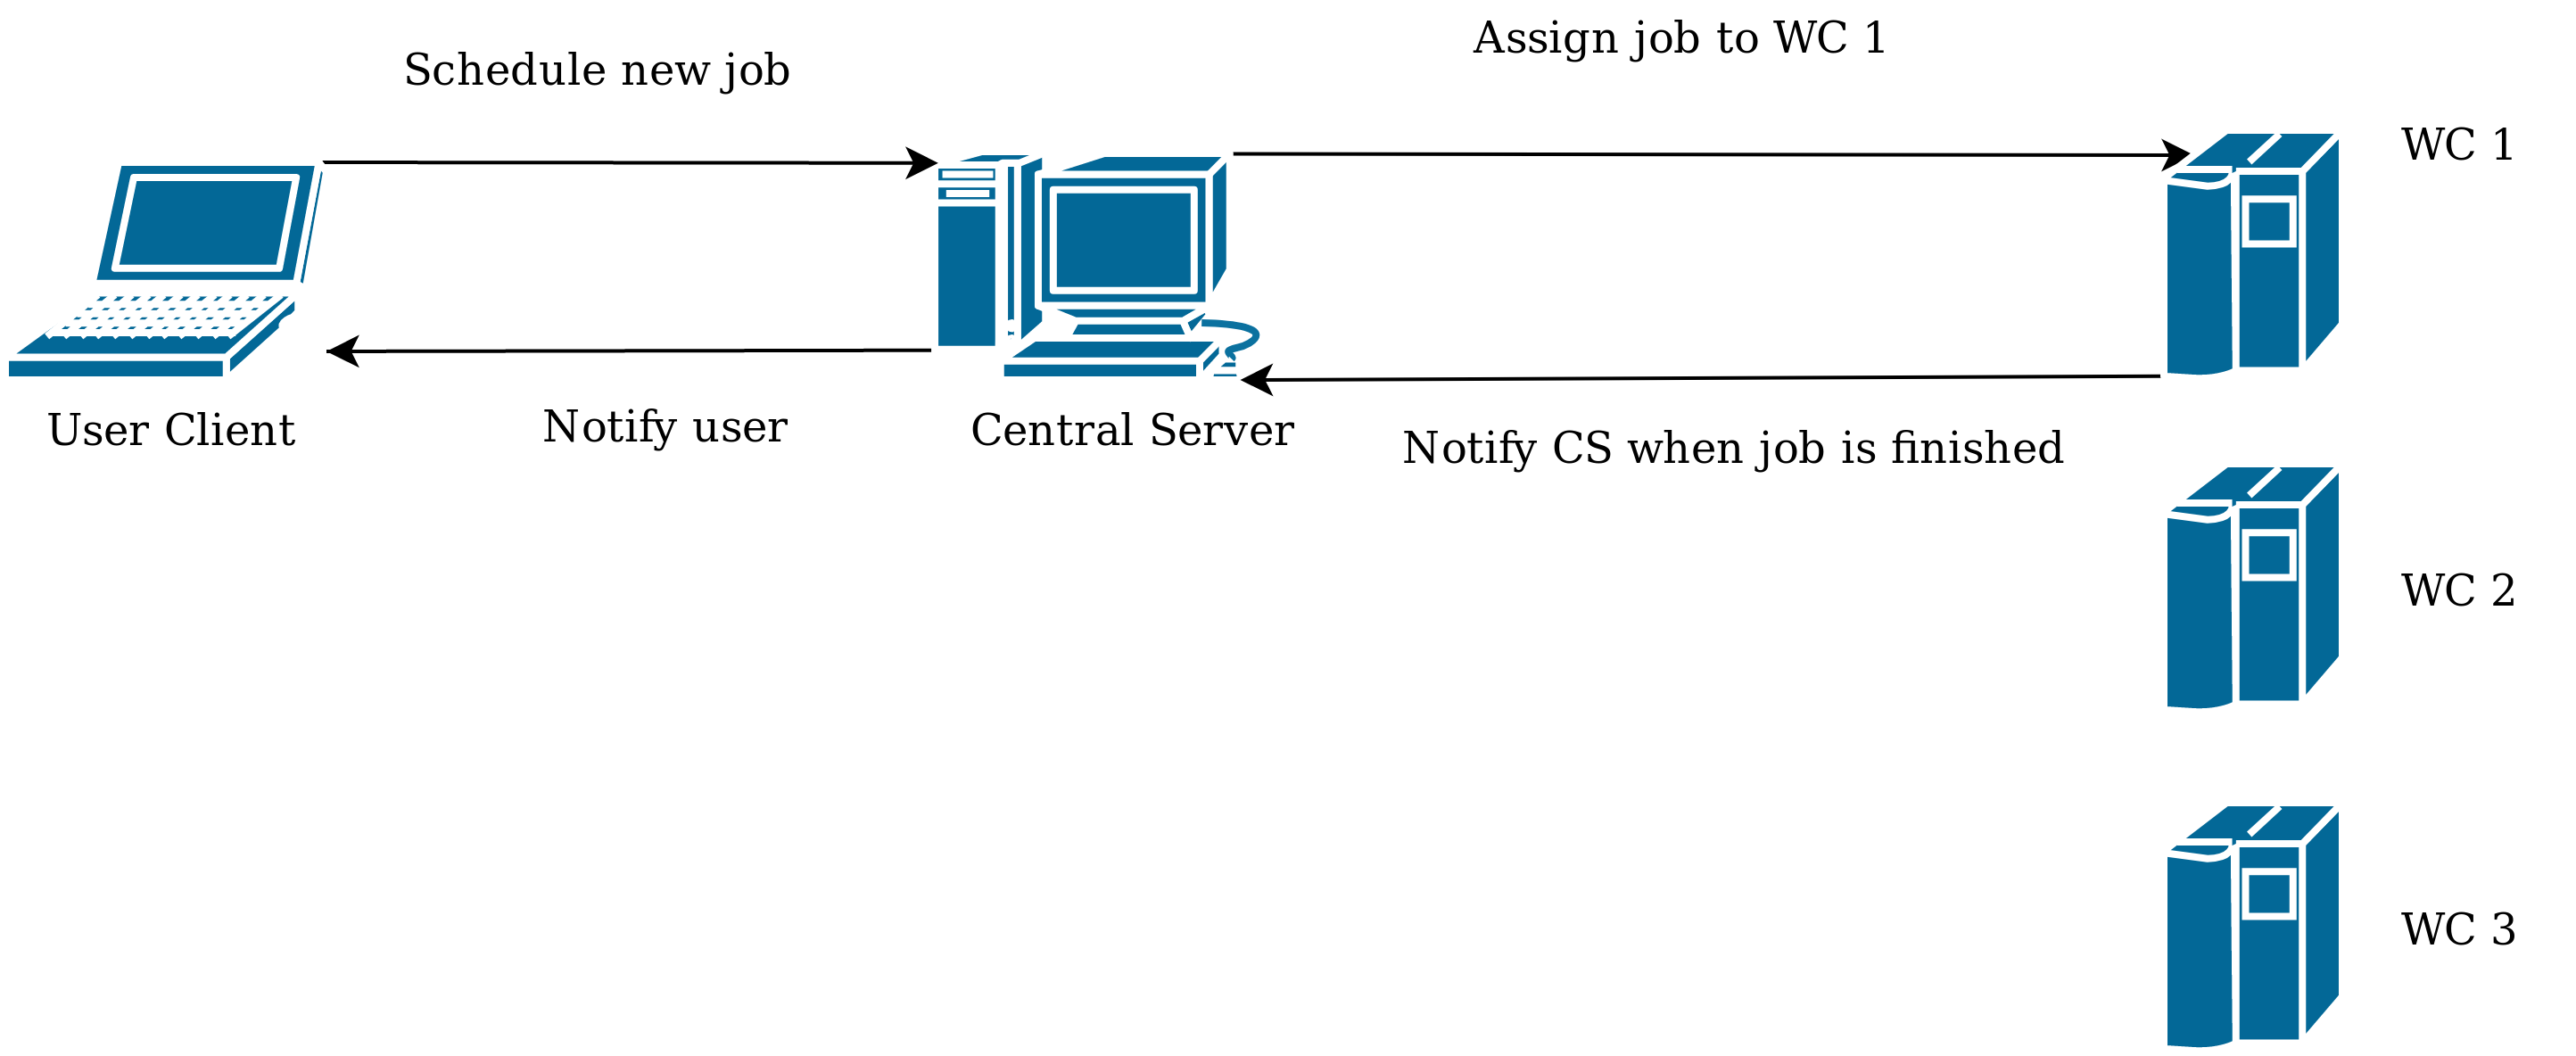
\includegraphics[width=\linewidth]{./system/systemmodel/images/schedulejob.png}
  \label{new-job}
  \caption{This diagram depicts how a user schedules a job, which the CS distributes to WC 1.
  In that case CS knows that there are enough resurces on WC 1 to execute users job.
  At the end the CS notifies the user that the job has finished.}
\end{figure}

\begin{figure}
  \subsubsection{Access a job}
  \centering
  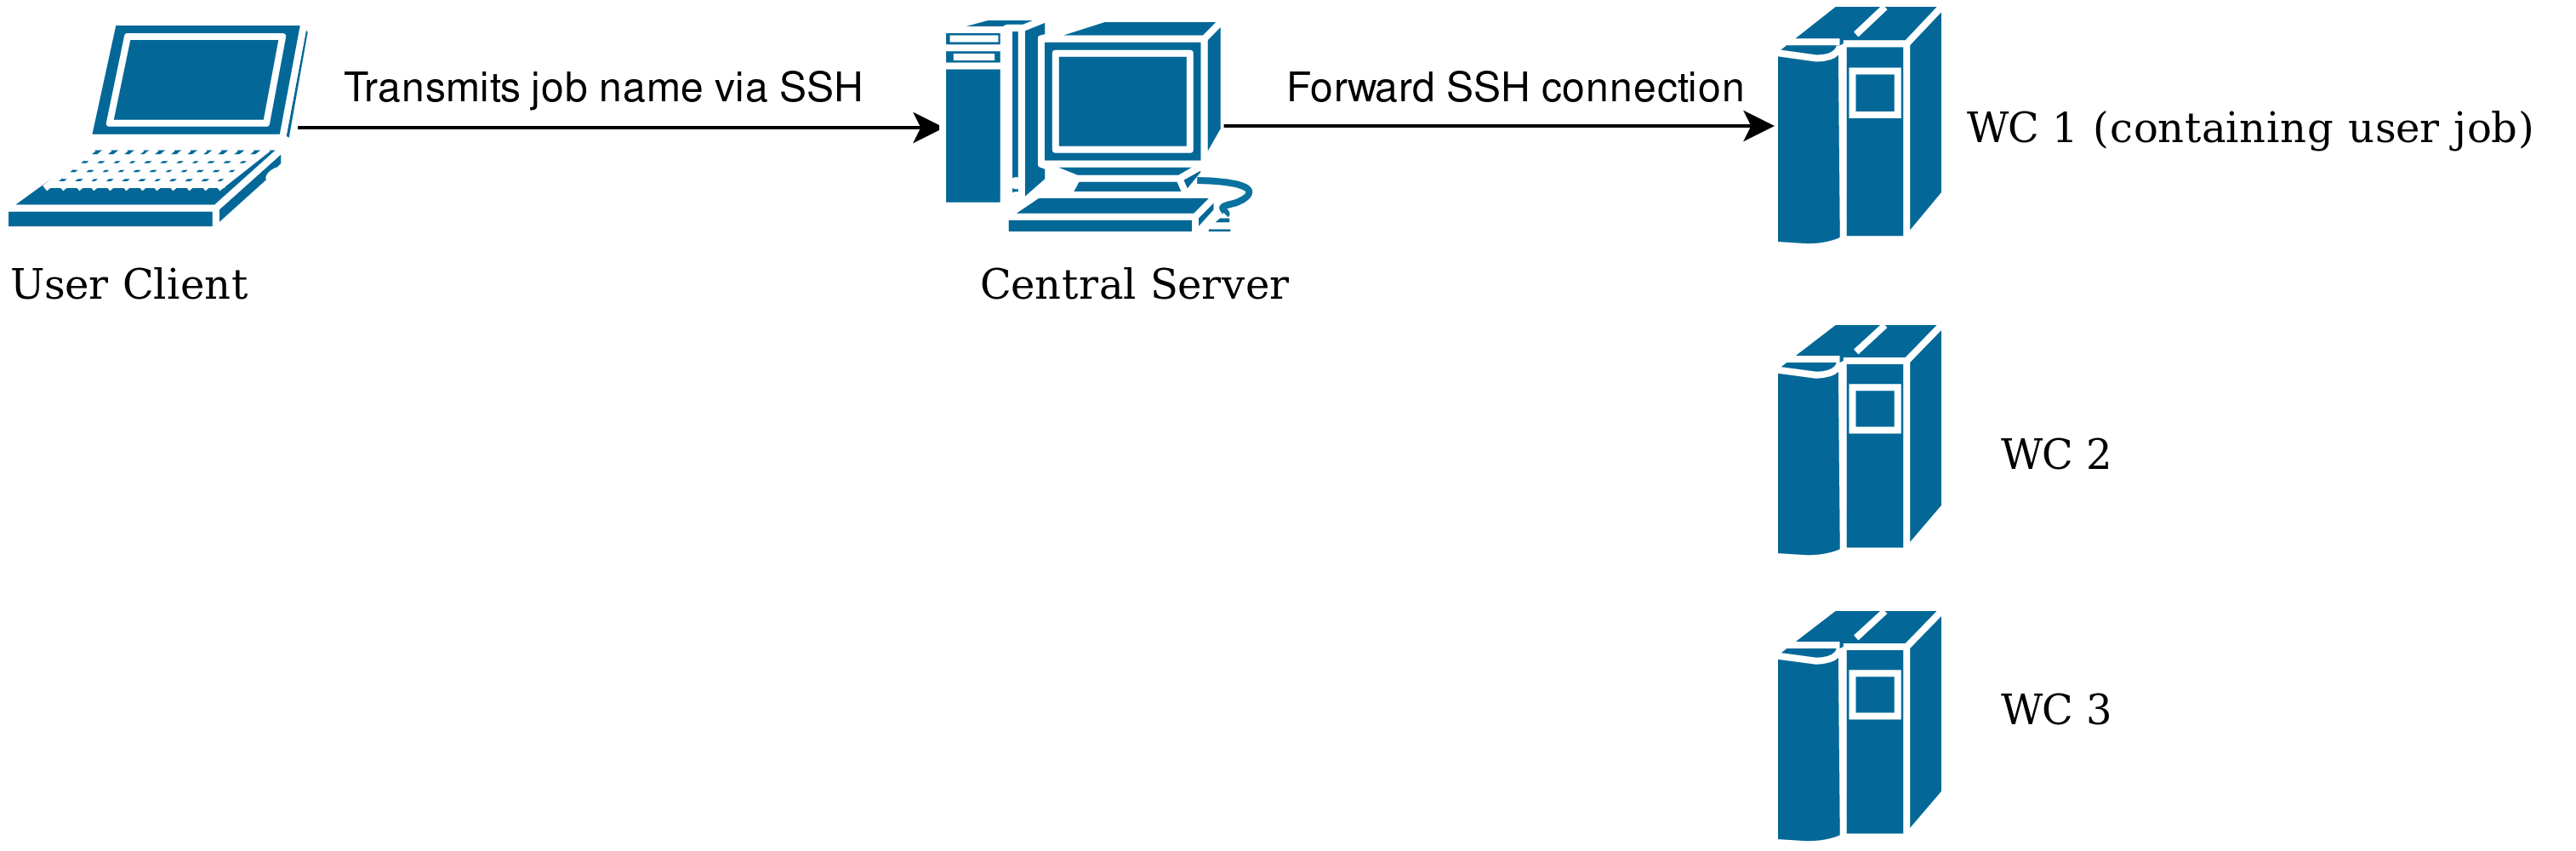
\includegraphics[width=\linewidth]{./system/systemmodel/images/accessjob.png}
  \label{access-job}
  \caption{This diagram depicts how a user accesses his job.
  The user has a job on one of the work machines that he wants to connect to.
  The user does not establish a direct connection with the WC.
  The user establishes an SSH connection to the server.
  This connection authenticates the user.
  It is also used to transmit the name of the job that the user wants to connect to.
  The server looks up which work machine the user's job is located on and forwards the SSH connection to that work machine.
  Finally, the SSH connection to the work machine is forwarded to the container with the user's job.}
\end{figure}

\begin{figure}
  \subsubsection{Get statistics}
  \centering
  
\includegraphics[width=0.5\linewidth]{./system/systemmodel/images/statistics.png}
  \label{statistics}
  \caption{This diagram depicts how a user accesses the statistics saved on the server.}
\end{figure}


\printunsrtglossaries
\end{document}


\newpage
\subsection{Use Case Diagram}
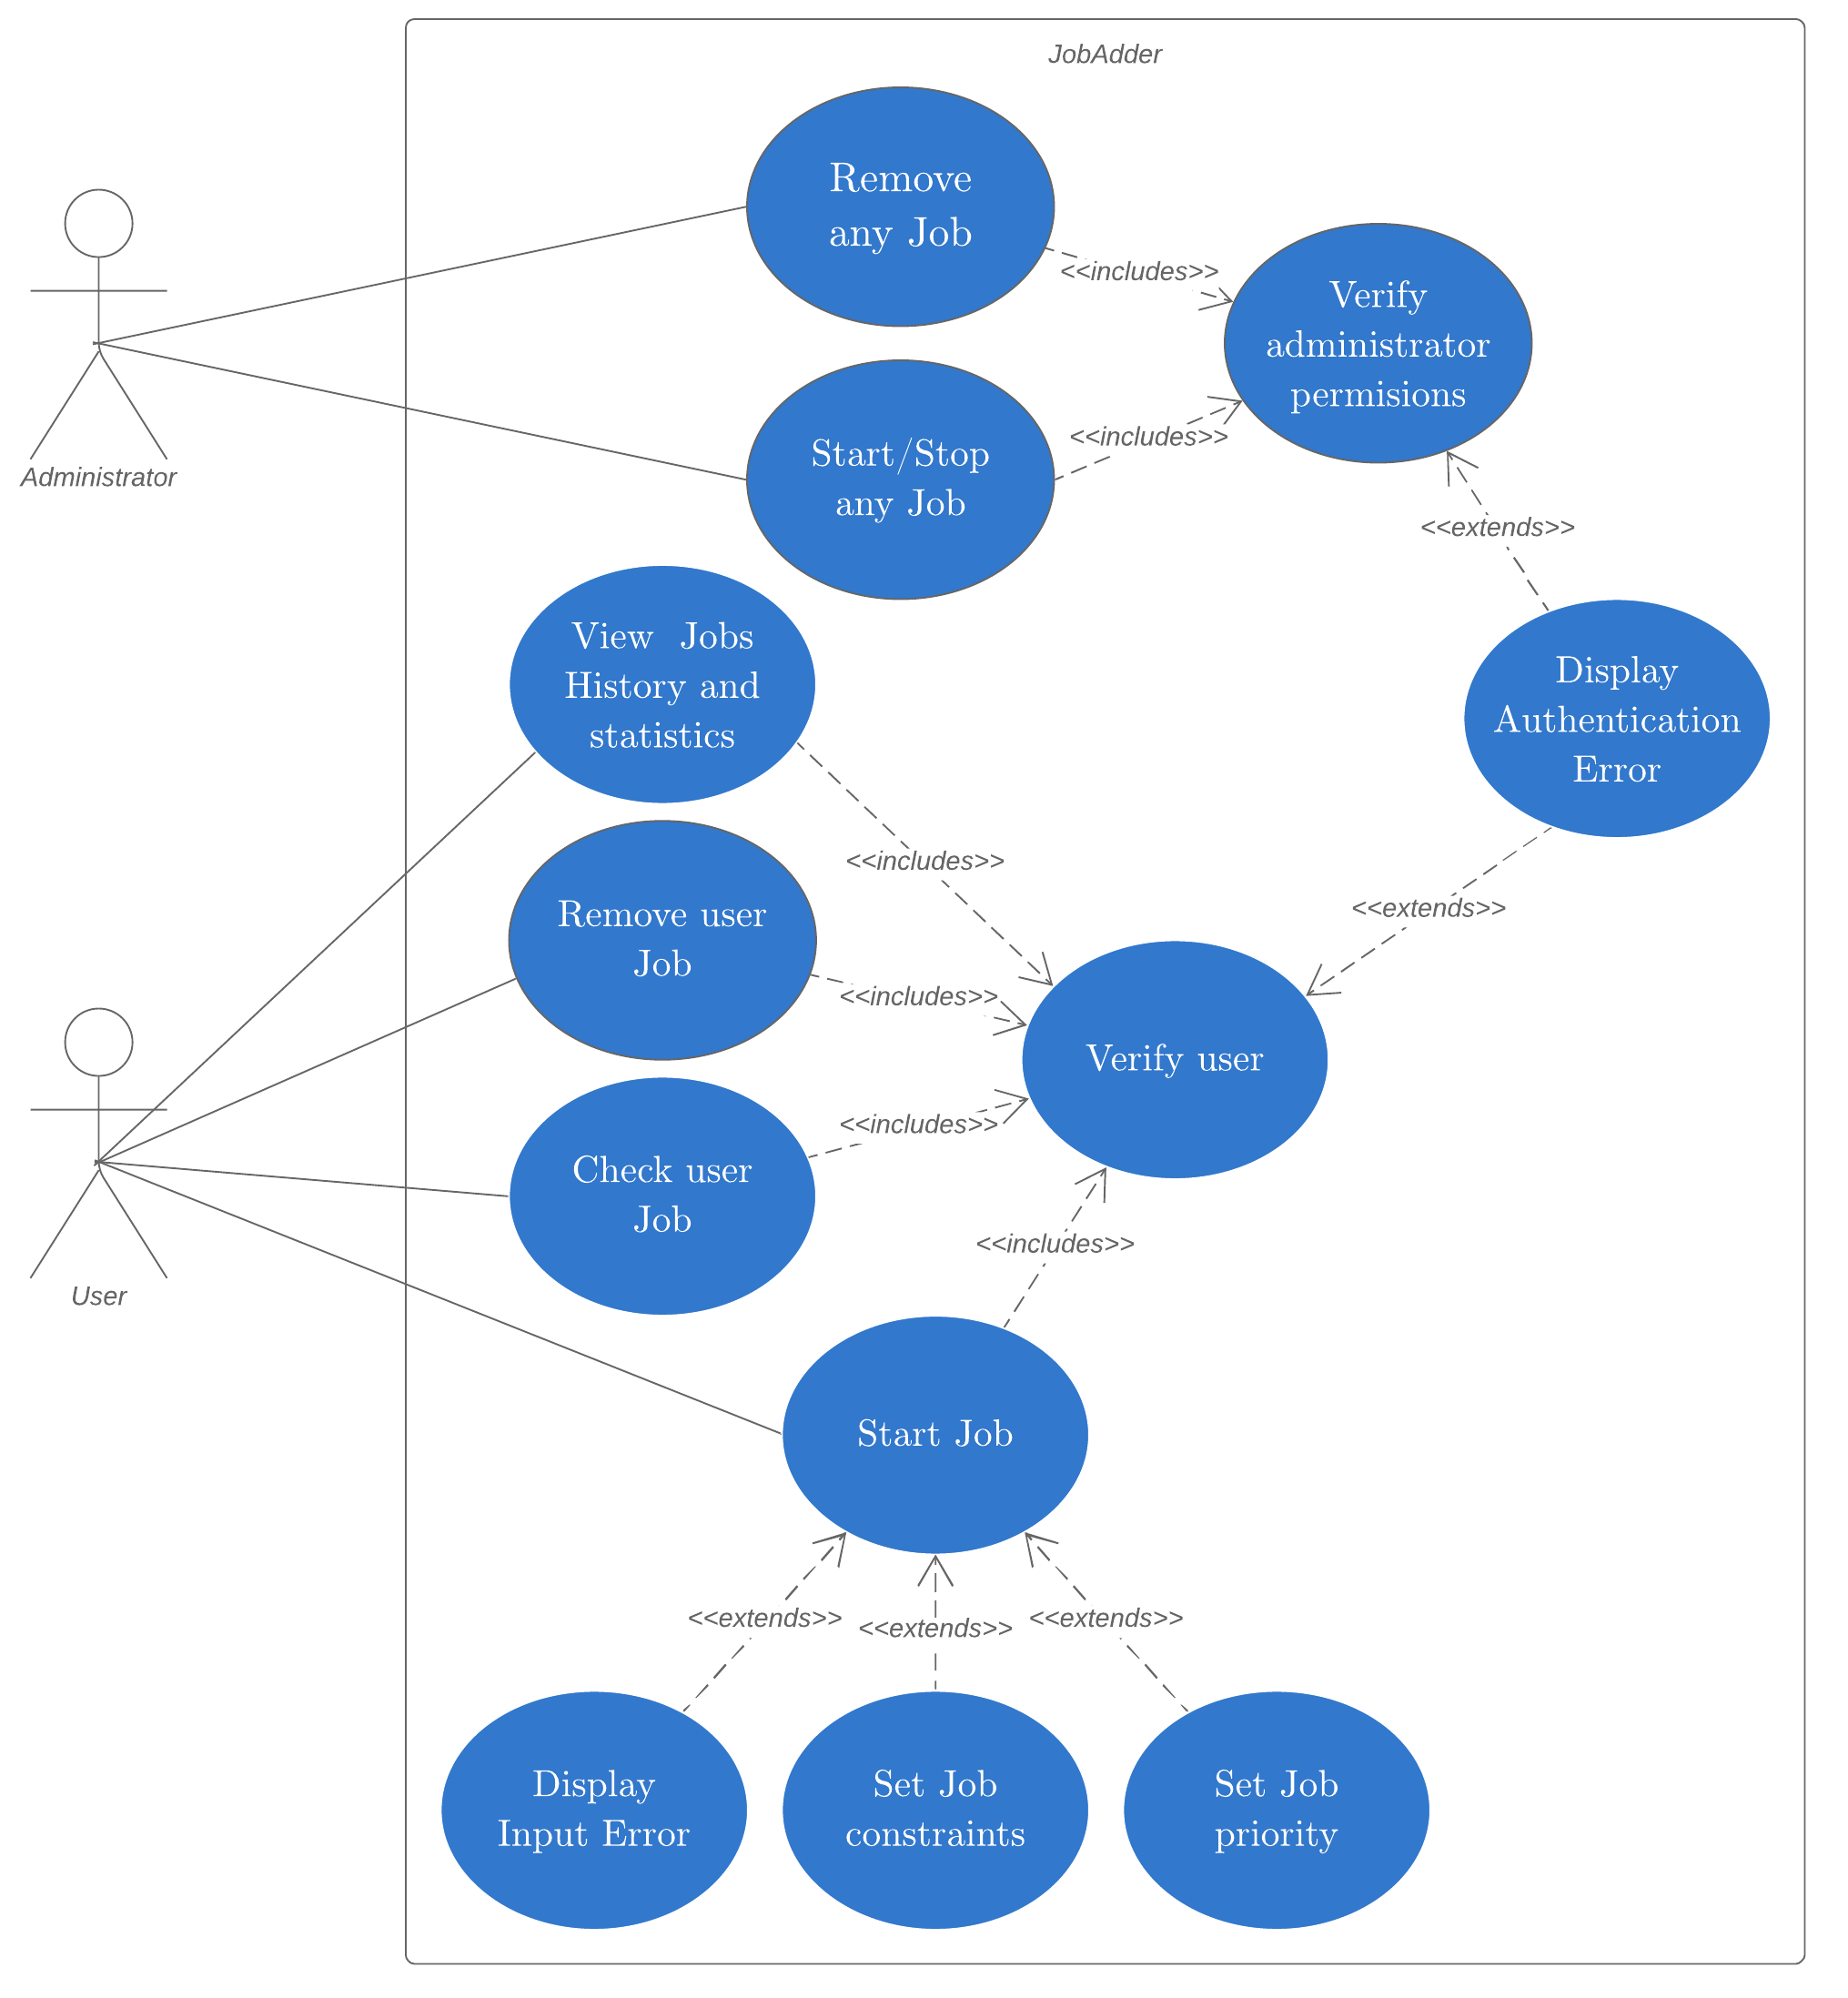
\includegraphics[width=\linewidth]{./system/systemmodel/images/usecasediagram.png}

\subsection{System Model}
\begin{figure}
  \subsubsection{Schedule new Job}
  \centering
  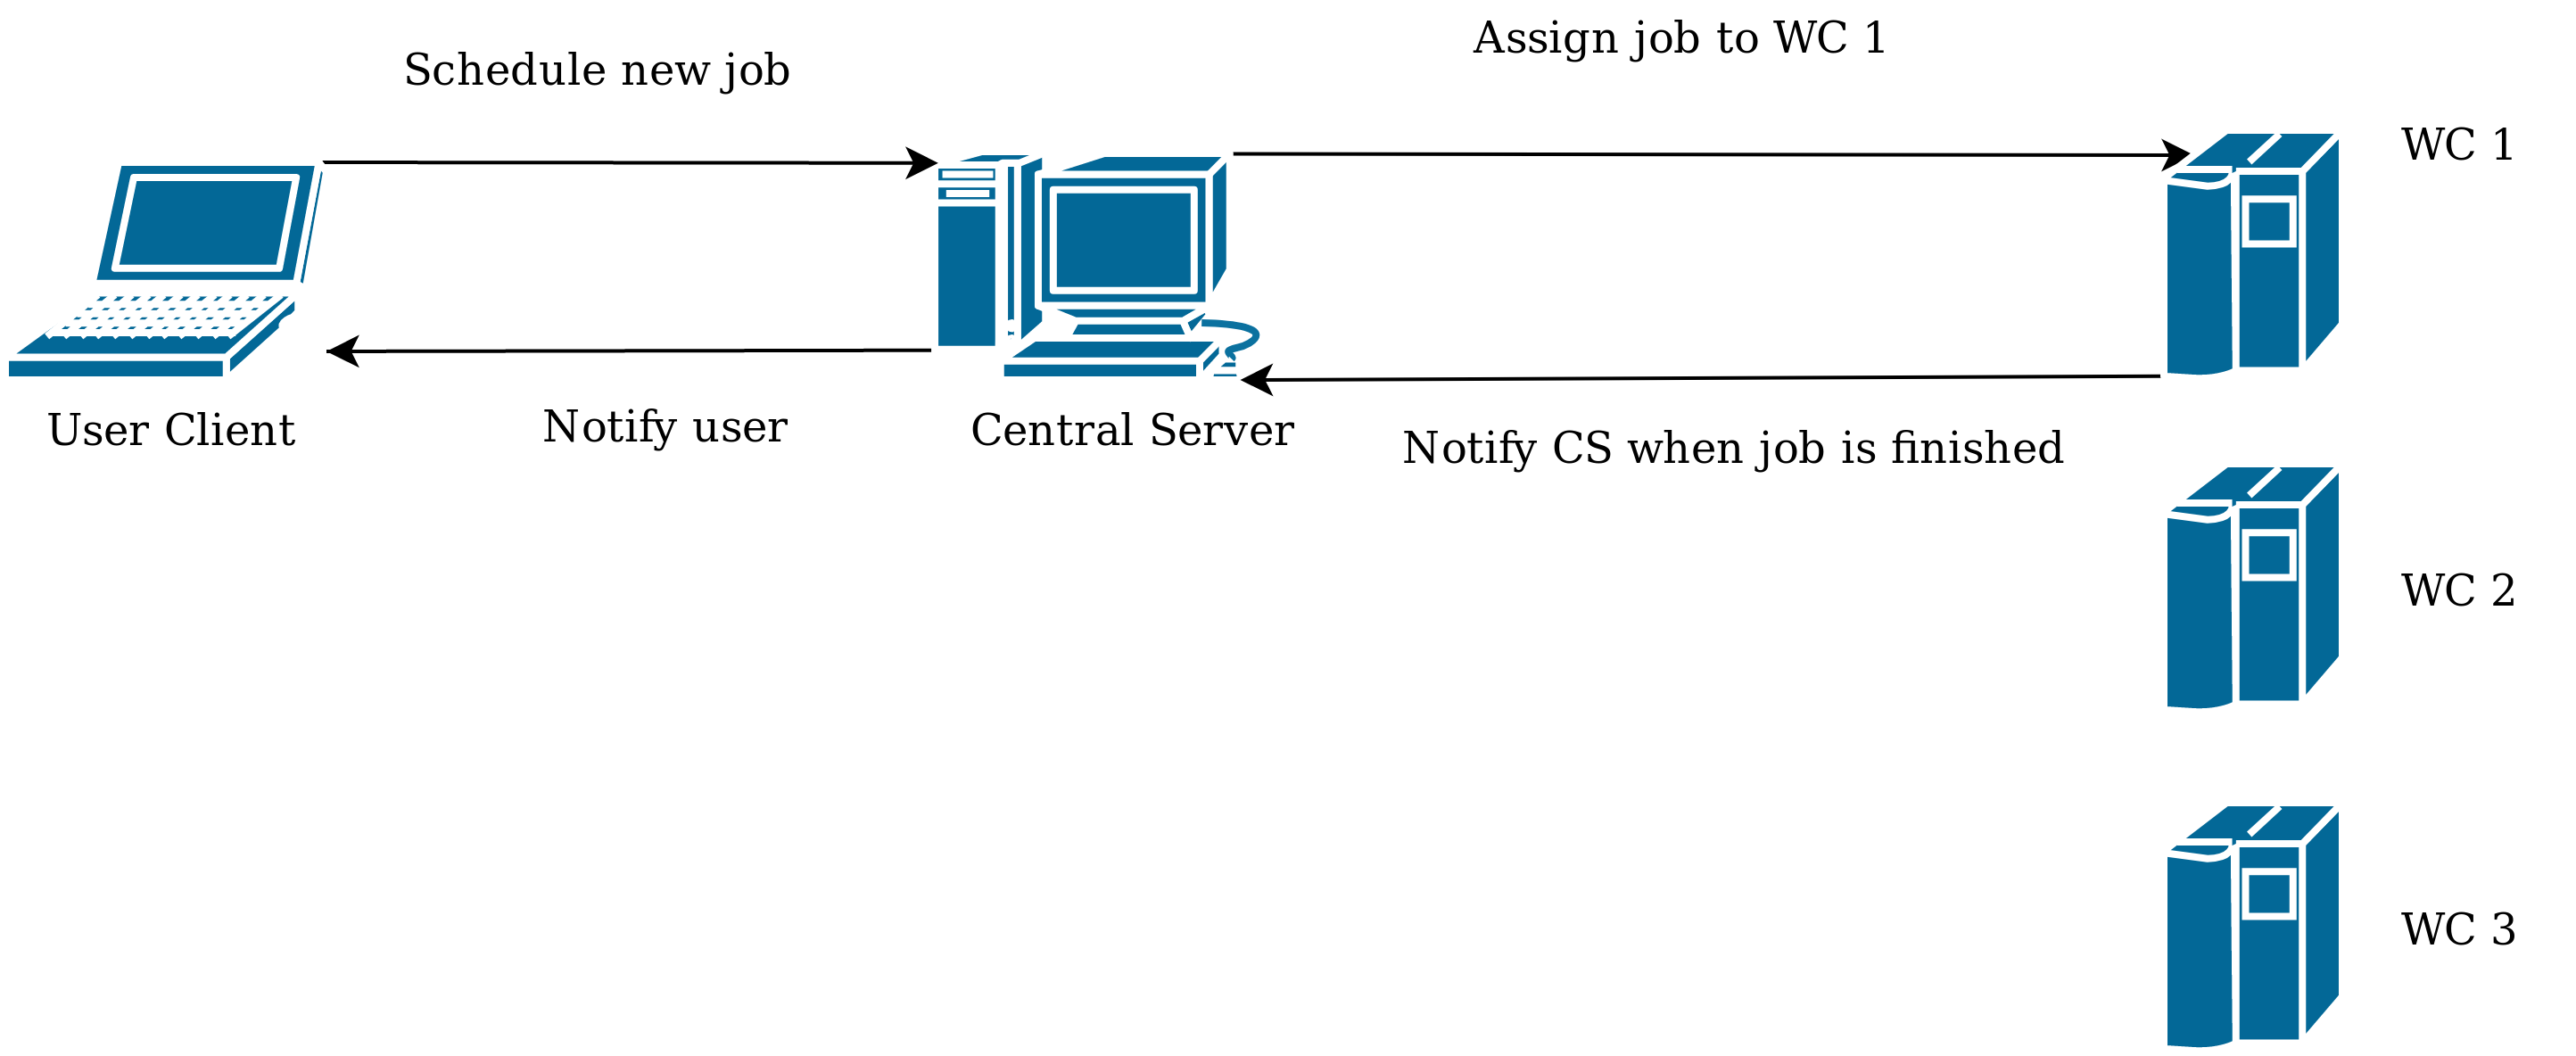
\includegraphics[width=\linewidth]{./system/systemmodel/images/schedulejob.png}
  \label{new-job}
  \caption{This diagram depicts how a user schedules a job, which the CS distributes to WC 1.
  In that case CS knows that there are enough resurces on WC 1 to execute users job.
  At the end the CS notifies the user that the job has finished.}
\end{figure}

\begin{figure}
  \subsubsection{Access a job}
  \centering
  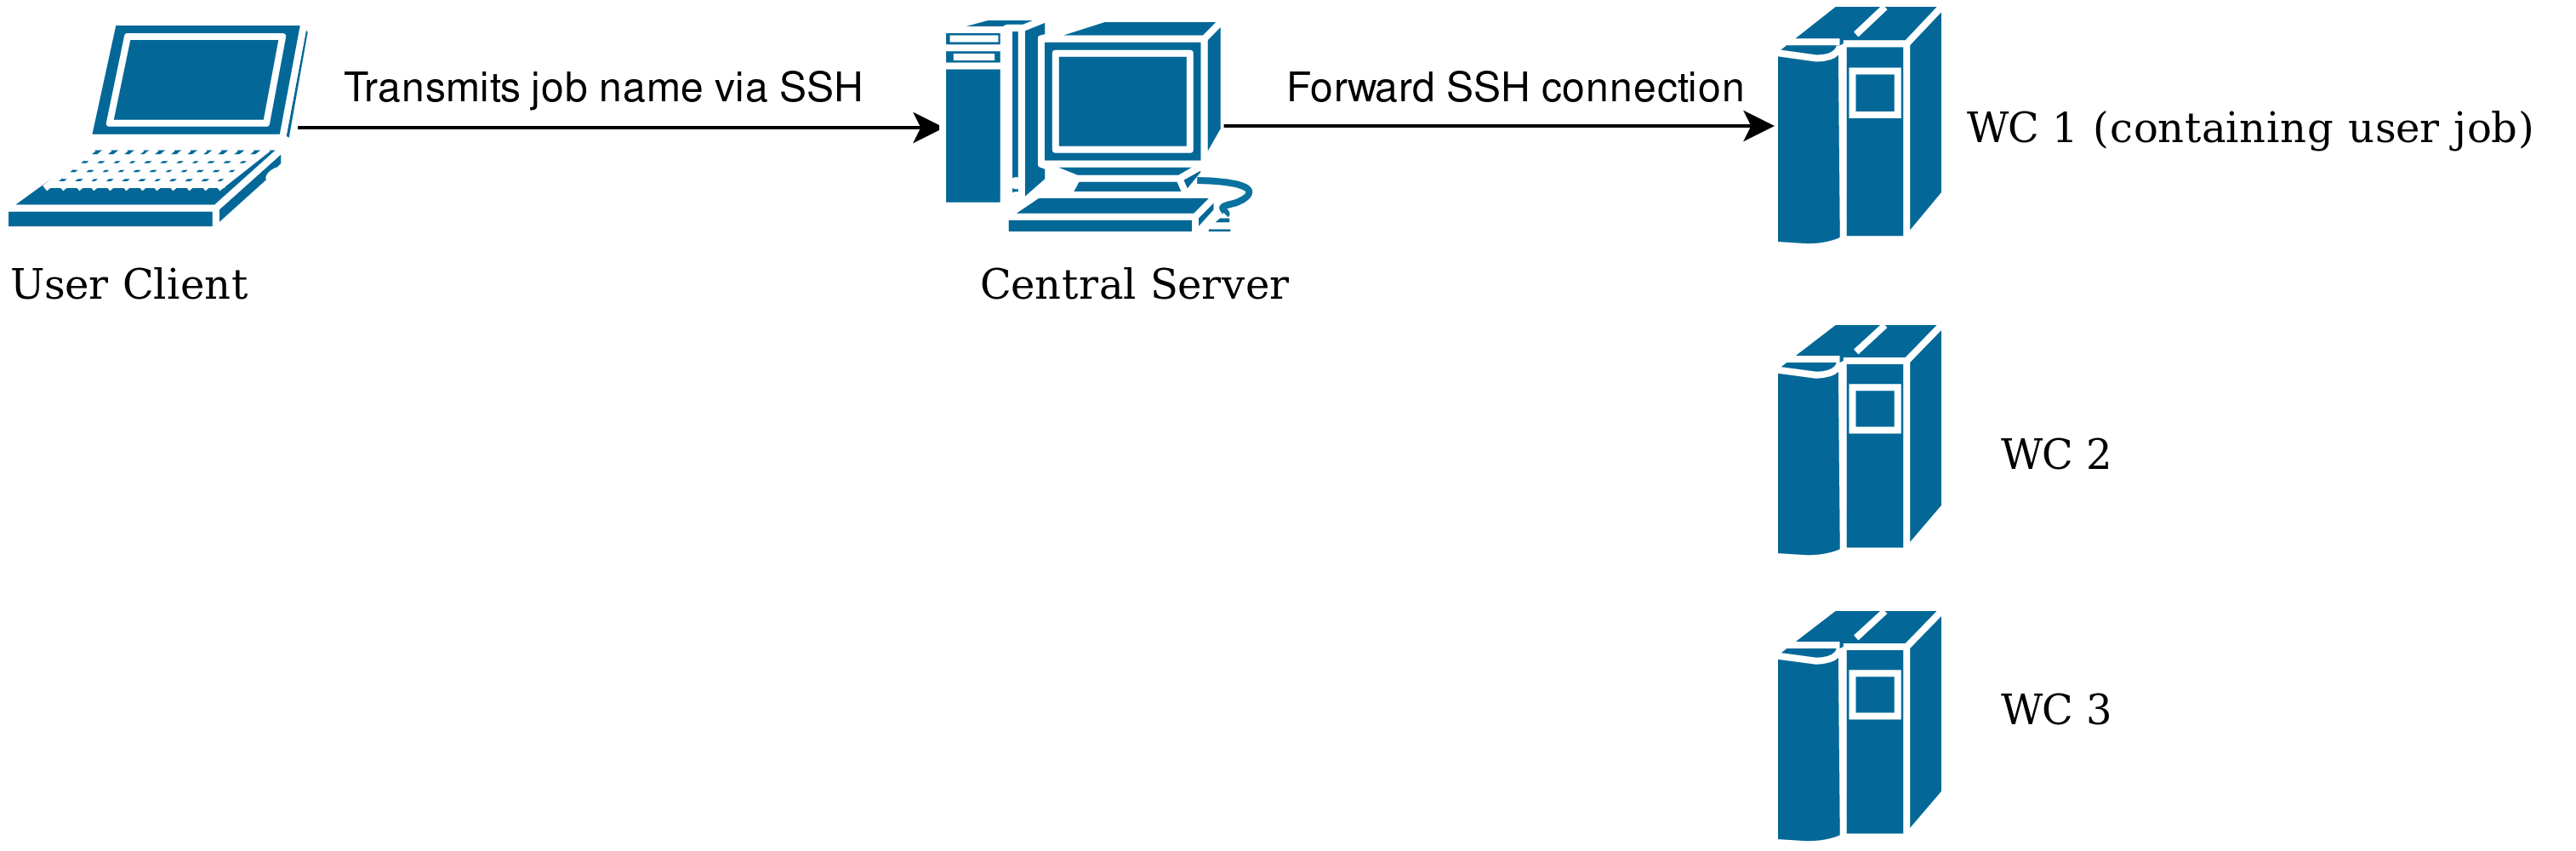
\includegraphics[width=\linewidth]{./system/systemmodel/images/accessjob.png}
  \label{access-job}
  \caption{This diagram depicts how a user accesses his job.
  The user has a job on one of the work machines that he wants to connect to.
  The user does not establish a direct connection with the WC.
  The user establishes an SSH connection to the server.
  This connection authenticates the user.
  It is also used to transmit the name of the job that the user wants to connect to.
  The server looks up which work machine the user's job is located on and forwards the SSH connection to that work machine.
  Finally, the SSH connection to the work machine is forwarded to the container with the user's job.}
\end{figure}

\begin{figure}
  \subsubsection{Get statistics}
  \centering
  
\includegraphics[width=0.5\linewidth]{./system/systemmodel/images/statistics.png}
  \label{statistics}
  \caption{This diagram depicts how a user accesses the statistics saved on the server.}
\end{figure}


\printunsrtglossaries
\end{document}


\newpage
\printunsrtglossaries
\end{document}
